\documentclass[final,5p,times,twocolumn]{elsarticle}

\usepackage{amsmath,amssymb,amsfonts,amsthm}
\usepackage{graphicx}
\usepackage{booktabs}
\usepackage{float}
\usepackage{array}
\usepackage[ruled,vlined,linesnumbered]{algorithm2e}
\usepackage{tikz}
\usetikzlibrary{positioning,arrows.meta,fit,backgrounds,calc,shapes.geometric}
\definecolor{tnblue}{HTML}{2A78D6}
\definecolor{tndark}{HTML}{104281}
\usepackage[hidelinks]{hyperref}
\usepackage{siunitx}
\sisetup{detect-weight=true,detect-family=true,per-mode=symbol,group-separator={,}}

\setcounter{topnumber}{3}\setcounter{bottomnumber}{2}\setcounter{totalnumber}{4}
\renewcommand{\topfraction}{0.9}\renewcommand{\bottomfraction}{0.5}
\renewcommand{\textfraction}{0.15}\renewcommand{\floatpagefraction}{0.7}
\renewcommand{\dbltopfraction}{0.9}\renewcommand{\dblfloatpagefraction}{0.8}\setcounter{dbltopnumber}{3}
\raggedbottom
\makeatletter % float-only pages: pack the floats at the top
\setlength{\@fptop}{0pt}\setlength{\@fpsep}{14pt plus 2pt}\setlength{\@fpbot}{0pt plus 1fil}
\setlength{\@dblfptop}{0pt}\setlength{\@dblfpsep}{14pt plus 2pt}\setlength{\@dblfpbot}{0pt plus 1fil}
\makeatother
\setlength{\textfloatsep}{12pt plus 2pt minus 4pt}

\theoremstyle{plain}
\newtheorem{proposition}{Proposition}

\DeclareMathOperator{\Var}{Var}
\DeclareMathOperator{\Cov}{Cov}
\DeclareMathOperator*{\argmax}{arg\,max}
\DeclareMathOperator*{\argmin}{arg\,min}
\DeclareMathOperator{\tr}{tr}
\newcommand{\btheta}{\boldsymbol{\theta}}
\newcommand{\bv}{\mathbf{v}}
\newcommand{\PL}{P_{L}}
\newcommand{\PLz}{P_{L_0}}
\newcommand{\R}{\mathbb{R}}
\newcommand{\E}{\mathbb{E}}
\newcommand{\ind}{\mathbf{1}} % indicator function

% generated by paper/scripts/make_assets.py -- do not edit
\newcommand{\sionnaVersion}{2.1.0}
\newcommand{\rtSamples}{\num{1e8}}
\newcommand{\rtDepth}{5}
\newcommand{\cellSize}{10}
\newcommand{\maxPl}{150}
\newcommand{\sceneSize}{3}
\newcommand{\siteMast}{6}
\newcommand{\ueHeight}{1.5}
\newcommand{\overtureRelease}{2026-09-23.0}
\newcommand{\rtHours}{4.7}
\newcommand{\rtSecPerSite}{77}
\newcommand{\rtBackend}{CPU (LLVM)}
\newcommand{\minSep}{250}
\newcommand{\cappedLo}{12}
\newcommand{\cappedHi}{45}
\newcommand{\matList}{brick, concrete, marble, metal, wood}
\newcommand{\nMat}{5}
\newcommand{\tileSize}{100}
\newcommand{\refDist}{100}
\newcommand{\minLinks}{30}
\newcommand{\freqGHz}{3.5}
\newcommand{\nCities}{11}
\newcommand{\nSamples}{8{,}977{,}400}
\newcommand{\nSamplesM}{9.0}
\newcommand{\nSites}{220}
\newcommand{\nSitesPerCity}{20}
\newcommand{\nTiles}{10{,}428}
\newcommand{\nBuildings}{105{,}800}
\newcommand{\qcRemoved}{1{,}170}
\newcommand{\qcShare}{0.013}
\newcommand{\impMin}{2}
\newcommand{\impMax}{50}
\newcommand{\impMinCity}{New York}
\newcommand{\impMaxCity}{London}
\newcommand{\siteHMedMin}{38}
\newcommand{\siteHMedMax}{318}
\newcommand{\siteHMedMinCity}{Munich}
\newcommand{\siteHMedMaxCity}{New York}
\newcommand{\siteHMax}{478}
\newcommand{\siteHMaxCity}{New York}
\newcommand{\siteHMedianAll}{51}
\newcommand{\betweenSd}{0.27}
\newcommand{\withinSdMin}{0.60}
\newcommand{\withinSdMax}{0.96}
\newcommand{\betweenWithinRatio}{0.3}
\newcommand{\gammaMedMin}{2.39}
\newcommand{\gammaMedMax}{3.15}
\newcommand{\gammaMedMinCity}{Vienna}
\newcommand{\gammaMedMaxCity}{Hamburg}
\newcommand{\olsMin}{\ensuremath{-}4.8}
\newcommand{\olsMax}{8.8}
\newcommand{\ebMin}{\ensuremath{-}0.90}
\newcommand{\ebMax}{6.45}
\newcommand{\fitRmseMin}{11.2}
\newcommand{\fitRmseMax}{12.7}
\newcommand{\shrinkMedian}{0.36}
\newcommand{\tauMin}{0.79}
\newcommand{\tauMax}{1.19}
\newcommand{\cityGammaMin}{0.81}
\newcommand{\cityGammaMinCity}{Chicago}
\newcommand{\nCityGammaBelowTwo}{4}
\newcommand{\medianSitesPerTile}{18}
\newcommand{\nDescLive}{32}
\newcommand{\topDesc}{footprint density}
\newcommand{\topDescR}{\ensuremath{-}0.45}
\newcommand{\maxAbsR}{0.45}
\newcommand{\qcMargin}{6}
\newcommand{\sinrFloor}{-20}
\newcommand{\kappaLink}{50}
\newcommand{\nInnerExpensive}{3}
\newcommand{\isdMain}{720}
\newcommand{\sceneArea}{9}
\newcommand{\areaPerSite}{0.45}
\newcommand{\areaPerSiteSmall}{0.9}
\newcommand{\nSitesWord}{Twenty}
\newcommand{\isdSmall}{1020}
\newcommand{\freqTwoGHz}{7.5}
\newcommand{\nRandCities}{4}
\newcommand{\randCities}{Amsterdam, London, New York, Paris}
\newcommand{\figCity}{Amsterdam}
\newcommand{\rmseMedian}{0.871}
\newcommand{\sdMedian}{0.098}
\newcommand{\plRmseMedian}{13.8}
\newcommand{\rmseUmaLos}{1.003}
\newcommand{\sdUmaLos}{0.147}
\newcommand{\plRmseUmaLos}{21.6}
\newcommand{\rmseUmaNlos}{1.453}
\newcommand{\sdUmaNlos}{0.234}
\newcommand{\plRmseUmaNlos}{13.8}
\newcommand{\rmseCost}{1.057}
\newcommand{\sdCost}{0.190}
\newcommand{\plRmseCost}{17.9}
\newcommand{\rmseKernel}{0.801}
\newcommand{\sdKernel}{0.107}
\newcommand{\plRmseKernel}{10.2}
\newcommand{\rmseGpArd}{0.762}
\newcommand{\sdGpArd}{0.081}
\newcommand{\plRmseGpArd}{9.5}
\newcommand{\rmseKnn}{0.777}
\newcommand{\sdKnn}{0.096}
\newcommand{\plRmseKnn}{9.7}
\newcommand{\rmseRidge}{0.765}
\newcommand{\sdRidge}{0.086}
\newcommand{\plRmseRidge}{9.6}
\newcommand{\rmseCoral}{0.789}
\newcommand{\sdCoral}{0.082}
\newcommand{\plRmseCoral}{10.3}
\newcommand{\rmseMlp}{0.768}
\newcommand{\sdMlp}{0.087}
\newcommand{\plRmseMlp}{9.5}
\newcommand{\rmseEncoder}{0.766}
\newcommand{\sdEncoder}{0.087}
\newcommand{\plRmseEncoder}{9.6}
\newcommand{\rmseGbdt}{0.764}
\newcommand{\sdGbdt}{0.077}
\newcommand{\plRmseGbdt}{9.5}
\newcommand{\rmseGbdtIw}{0.772}
\newcommand{\sdGbdtIw}{0.079}
\newcommand{\plRmseGbdtIw}{9.5}
\newcommand{\bestZeroShot}{GP-ARD}
\newcommand{\gainGbdtMedian}{12.2}
\newcommand{\gainKernelMedian}{8.0}
\newcommand{\hardCity}{Chicago}
\newcommand{\hardCityBest}{0.834}
\newcommand{\hardCityBestOp}{Source median}
\newcommand{\sigmaMin}{0.1}
\newcommand{\sigmaMax}{0.2}
\newcommand{\hBsMedian}{56}
\newcommand{\iwEssMin}{12}
\newcommand{\iwEssMax}{76}
\newcommand{\nBetterThanMedian}{9}
\newcommand{\nOps}{13}
\newcommand{\knnKMedian}{200}
\newcommand{\nSigmaLargest}{9}
\newcommand{\linkTreesMedian}{83}
\newcommand{\linkClfTreesMedian}{82}
\newcommand{\dGbdtMedian}{\ensuremath{-}0.106}
\newcommand{\loGbdtMedian}{\ensuremath{-}0.157}
\newcommand{\hiGbdtMedian}{\ensuremath{-}0.052}
\newcommand{\pGbdtMedian}{0.010}
\newcommand{\nGbdtMedian}{9}
\newcommand{\holmGbdtMedian}{not significant}
\newcommand{\dKernelMedian}{\ensuremath{-}0.070}
\newcommand{\loKernelMedian}{\ensuremath{-}0.129}
\newcommand{\hiKernelMedian}{\ensuremath{-}0.001}
\newcommand{\pKernelMedian}{0.083}
\newcommand{\nKernelMedian}{9}
\newcommand{\holmKernelMedian}{not significant}
\newcommand{\dRidgeMedian}{\ensuremath{-}0.105}
\newcommand{\loRidgeMedian}{\ensuremath{-}0.158}
\newcommand{\hiRidgeMedian}{\ensuremath{-}0.047}
\newcommand{\pRidgeMedian}{0.010}
\newcommand{\nRidgeMedian}{9}
\newcommand{\holmRidgeMedian}{not significant}
\newcommand{\dMlpMedian}{\ensuremath{-}0.103}
\newcommand{\loMlpMedian}{\ensuremath{-}0.157}
\newcommand{\hiMlpMedian}{\ensuremath{-}0.043}
\newcommand{\pMlpMedian}{0.010}
\newcommand{\nMlpMedian}{9}
\newcommand{\holmMlpMedian}{not significant}
\newcommand{\dGpMedian}{\ensuremath{-}0.108}
\newcommand{\loGpMedian}{\ensuremath{-}0.159}
\newcommand{\hiGpMedian}{\ensuremath{-}0.053}
\newcommand{\pGpMedian}{0.007}
\newcommand{\nGpMedian}{9}
\newcommand{\holmGpMedian}{not significant}
\newcommand{\dEncMedian}{\ensuremath{-}0.105}
\newcommand{\loEncMedian}{\ensuremath{-}0.157}
\newcommand{\hiEncMedian}{\ensuremath{-}0.048}
\newcommand{\pEncMedian}{0.010}
\newcommand{\nEncMedian}{9}
\newcommand{\holmEncMedian}{not significant}
\newcommand{\dGbdtKernel}{\ensuremath{-}0.037}
\newcommand{\loGbdtKernel}{\ensuremath{-}0.061}
\newcommand{\hiGbdtKernel}{\ensuremath{-}0.016}
\newcommand{\pGbdtKernel}{0.005}
\newcommand{\nGbdtKernel}{10}
\newcommand{\holmGbdtKernel}{significant}
\newcommand{\dGpKernel}{\ensuremath{-}0.039}
\newcommand{\loGpKernel}{\ensuremath{-}0.063}
\newcommand{\hiGpKernel}{\ensuremath{-}0.021}
\newcommand{\pGpKernel}{0.002}
\newcommand{\nGpKernel}{10}
\newcommand{\holmGpKernel}{significant}
\newcommand{\dIwGbdt}{+0.008}
\newcommand{\loIwGbdt}{+0.003}
\newcommand{\hiIwGbdt}{+0.014}
\newcommand{\pIwGbdt}{0.007}
\newcommand{\nIwGbdt}{2}
\newcommand{\holmIwGbdt}{significant}
\newcommand{\dCoralRidge}{+0.024}
\newcommand{\loCoralRidge}{+0.001}
\newcommand{\hiCoralRidge}{+0.048}
\newcommand{\pCoralRidge}{0.102}
\newcommand{\nCoralRidge}{3}
\newcommand{\holmCoralRidge}{not significant}
\newcommand{\dFewGbdt}{\ensuremath{-}0.005}
\newcommand{\loFewGbdt}{\ensuremath{-}0.011}
\newcommand{\hiFewGbdt}{\ensuremath{-}0.001}
\newcommand{\pFewGbdt}{0.032}
\newcommand{\nFewGbdt}{9}
\newcommand{\holmFewGbdt}{not significant}
\newcommand{\dFewRidge}{\ensuremath{-}0.005}
\newcommand{\loFewRidge}{\ensuremath{-}0.009}
\newcommand{\hiFewRidge}{\ensuremath{-}0.002}
\newcommand{\pFewRidge}{0.010}
\newcommand{\nFewRidge}{9}
\newcommand{\holmFewRidge}{not significant}
\newcommand{\dFewDesignGbdt}{\ensuremath{-}0.004}
\newcommand{\loFewDesignGbdt}{\ensuremath{-}0.010}
\newcommand{\hiFewDesignGbdt}{+0.001}
\newcommand{\pFewDesignGbdt}{0.278}
\newcommand{\nFewDesignGbdt}{8}
\newcommand{\holmFewDesignGbdt}{not significant}
\newcommand{\dFewEbGbdt}{\ensuremath{-}0.018}
\newcommand{\loFewEbGbdt}{\ensuremath{-}0.028}
\newcommand{\hiFewEbGbdt}{\ensuremath{-}0.006}
\newcommand{\pFewEbGbdt}{0.032}
\newcommand{\nFewEbGbdt}{10}
\newcommand{\holmFewEbGbdt}{not significant}
\newcommand{\dNetGbdtMedian}{\ensuremath{-}1.75}
\newcommand{\loNetGbdtMedian}{\ensuremath{-}2.27}
\newcommand{\hiNetGbdtMedian}{\ensuremath{-}1.26}
\newcommand{\pNetGbdtMedian}{$<$0.001}
\newcommand{\nNetGbdtMedian}{11}
\newcommand{\holmNetGbdtMedian}{significant}
\newcommand{\dNetLinkGbdt}{\ensuremath{-}3.44}
\newcommand{\loNetLinkGbdt}{\ensuremath{-}3.83}
\newcommand{\hiNetLinkGbdt}{\ensuremath{-}3.10}
\newcommand{\pNetLinkGbdt}{$<$0.001}
\newcommand{\nNetLinkGbdt}{11}
\newcommand{\holmNetLinkGbdt}{significant}
\newcommand{\dNetLinkOracle}{\ensuremath{-}2.33}
\newcommand{\loNetLinkOracle}{\ensuremath{-}2.63}
\newcommand{\hiNetLinkOracle}{\ensuremath{-}2.08}
\newcommand{\pNetLinkOracle}{$<$0.001}
\newcommand{\nNetLinkOracle}{11}
\newcommand{\holmNetLinkOracle}{significant}
\newcommand{\dNetLinkAssoc}{+18.3}
\newcommand{\loNetLinkAssoc}{+14.5}
\newcommand{\hiNetLinkAssoc}{+22.6}
\newcommand{\pNetLinkAssoc}{$<$0.001}
\newcommand{\nNetLinkAssoc}{11}
\newcommand{\holmNetLinkAssoc}{significant}
\newcommand{\dNetLinkOracleAssoc}{+18.4}
\newcommand{\loNetLinkOracleAssoc}{+14.6}
\newcommand{\hiNetLinkOracleAssoc}{+22.6}
\newcommand{\pNetLinkOracleAssoc}{$<$0.001}
\newcommand{\nNetLinkOracleAssoc}{11}
\newcommand{\holmNetLinkOracleAssoc}{significant}
\newcommand{\dNetLinkRegret}{\ensuremath{-}17.7}
\newcommand{\loNetLinkRegret}{\ensuremath{-}23.5}
\newcommand{\hiNetLinkRegret}{\ensuremath{-}12.6}
\newcommand{\pNetLinkRegret}{$<$0.001}
\newcommand{\nNetLinkRegret}{11}
\newcommand{\holmNetLinkRegret}{significant}
\newcommand{\dNetLinkOracleRegret}{\ensuremath{-}8.5}
\newcommand{\loNetLinkOracleRegret}{\ensuremath{-}11.1}
\newcommand{\hiNetLinkOracleRegret}{\ensuremath{-}5.9}
\newcommand{\pNetLinkOracleRegret}{$<$0.001}
\newcommand{\nNetLinkOracleRegret}{11}
\newcommand{\holmNetLinkOracleRegret}{significant}
\newcommand{\dNetLinkSinr}{\ensuremath{-}2.19}
\newcommand{\loNetLinkSinr}{\ensuremath{-}2.50}
\newcommand{\hiNetLinkSinr}{\ensuremath{-}1.93}
\newcommand{\pNetLinkSinr}{$<$0.001}
\newcommand{\nNetLinkSinr}{11}
\newcommand{\holmNetLinkSinr}{significant}
\newcommand{\dNetLinkCov}{+5.0}
\newcommand{\loNetLinkCov}{+2.5}
\newcommand{\hiNetLinkCov}{+7.8}
\newcommand{\pNetLinkCov}{$<$0.001}
\newcommand{\nNetLinkCov}{11}
\newcommand{\holmNetLinkCov}{significant}
\newcommand{\dNetLinkTwentyFive}{+0.03}
\newcommand{\loNetLinkTwentyFive}{+0.02}
\newcommand{\hiNetLinkTwentyFive}{+0.04}
\newcommand{\pNetLinkTwentyFive}{0.003}
\newcommand{\nNetLinkTwentyFive}{1}
\newcommand{\holmNetLinkTwentyFive}{significant}
\newcommand{\dNetFixedKappa}{+0.00}
\newcommand{\loNetFixedKappa}{\ensuremath{-}0.01}
\newcommand{\hiNetFixedKappa}{+0.00}
\newcommand{\pNetFixedKappa}{0.002}
\newcommand{\nNetFixedKappa}{10}
\newcommand{\holmNetFixedKappa}{significant}
\newcommand{\dNetDesignVar}{+0.21}
\newcommand{\loNetDesignVar}{+0.16}
\newcommand{\hiNetDesignVar}{+0.27}
\newcommand{\pNetDesignVar}{$<$0.001}
\newcommand{\nNetDesignVar}{0}
\newcommand{\holmNetDesignVar}{significant}
\newcommand{\dNetDesignStrat}{+0.07}
\newcommand{\loNetDesignStrat}{+0.03}
\newcommand{\hiNetDesignStrat}{+0.12}
\newcommand{\pNetDesignStrat}{0.005}
\newcommand{\nNetDesignStrat}{2}
\newcommand{\holmNetDesignStrat}{not significant}
\newcommand{\dDecHurdle}{+0.00}
\newcommand{\loDecHurdle}{+0.00}
\newcommand{\hiDecHurdle}{+0.00}
\newcommand{\pDecHurdle}{1.000}
\newcommand{\nDecHurdle}{0}
\newcommand{\holmDecHurdle}{not significant}
\newcommand{\dDecHurdleRegret}{\ensuremath{-}17.5}
\newcommand{\loDecHurdleRegret}{\ensuremath{-}23.3}
\newcommand{\hiDecHurdleRegret}{\ensuremath{-}12.4}
\newcommand{\pDecHurdleRegret}{$<$0.001}
\newcommand{\nDecHurdleRegret}{11}
\newcommand{\holmDecHurdleRegret}{significant}
\newcommand{\dDecLos}{\ensuremath{-}1.79}
\newcommand{\loDecLos}{\ensuremath{-}2.19}
\newcommand{\hiDecLos}{\ensuremath{-}1.48}
\newcommand{\pDecLos}{$<$0.001}
\newcommand{\nDecLos}{11}
\newcommand{\holmDecLos}{significant}
\newcommand{\dDecLosAssoc}{+11.8}
\newcommand{\loDecLosAssoc}{+9.2}
\newcommand{\hiDecLosAssoc}{+15.2}
\newcommand{\pDecLosAssoc}{$<$0.001}
\newcommand{\nDecLosAssoc}{11}
\newcommand{\holmDecLosAssoc}{significant}
\newcommand{\dDecLosH}{\ensuremath{-}1.79}
\newcommand{\loDecLosH}{\ensuremath{-}2.19}
\newcommand{\hiDecLosH}{\ensuremath{-}1.48}
\newcommand{\pDecLosH}{$<$0.001}
\newcommand{\nDecLosH}{11}
\newcommand{\holmDecLosH}{significant}
\newcommand{\dDecLosHRegret}{+0.0}
\newcommand{\loDecLosHRegret}{+0.0}
\newcommand{\hiDecLosHRegret}{+0.0}
\newcommand{\pDecLosHRegret}{1.000}
\newcommand{\nDecLosHRegret}{0}
\newcommand{\holmDecLosHRegret}{not significant}
\newcommand{\dDecLinkBestTile}{\ensuremath{-}1.65}
\newcommand{\loDecLinkBestTile}{\ensuremath{-}1.81}
\newcommand{\hiDecLinkBestTile}{\ensuremath{-}1.50}
\newcommand{\pDecLinkBestTile}{$<$0.001}
\newcommand{\nDecLinkBestTile}{11}
\newcommand{\holmDecLinkBestTile}{significant}
\newcommand{\dDecLinkBestTileAssoc}{+6.3}
\newcommand{\loDecLinkBestTileAssoc}{+5.2}
\newcommand{\hiDecLinkBestTileAssoc}{+7.5}
\newcommand{\pDecLinkBestTileAssoc}{$<$0.001}
\newcommand{\nDecLinkBestTileAssoc}{11}
\newcommand{\holmDecLinkBestTileAssoc}{significant}
\newcommand{\dDecLinkBestTileRegret}{\ensuremath{-}0.2}
\newcommand{\loDecLinkBestTileRegret}{\ensuremath{-}0.4}
\newcommand{\hiDecLinkBestTileRegret}{+0.0}
\newcommand{\pDecLinkBestTileRegret}{0.250}
\newcommand{\nDecLinkBestTileRegret}{3}
\newcommand{\holmDecLinkBestTileRegret}{not significant}
\newcommand{\dDecLinkOracleLosH}{\ensuremath{-}0.70}
\newcommand{\loDecLinkOracleLosH}{\ensuremath{-}0.81}
\newcommand{\hiDecLinkOracleLosH}{\ensuremath{-}0.60}
\newcommand{\pDecLinkOracleLosH}{$<$0.001}
\newcommand{\nDecLinkOracleLosH}{11}
\newcommand{\holmDecLinkOracleLosH}{significant}
\newcommand{\dDecLinkOracleLosHAssoc}{+6.6}
\newcommand{\loDecLinkOracleLosHAssoc}{+5.3}
\newcommand{\hiDecLinkOracleLosHAssoc}{+8.0}
\newcommand{\pDecLinkOracleLosHAssoc}{$<$0.001}
\newcommand{\nDecLinkOracleLosHAssoc}{11}
\newcommand{\holmDecLinkOracleLosHAssoc}{significant}
\newcommand{\dDecLinkOracleLosHRegret}{+0.0}
\newcommand{\loDecLinkOracleLosHRegret}{+0.0}
\newcommand{\hiDecLinkOracleLosHRegret}{+0.1}
\newcommand{\pDecLinkOracleLosHRegret}{0.812}
\newcommand{\nDecLinkOracleLosHRegret}{3}
\newcommand{\holmDecLinkOracleLosHRegret}{not significant}
\newcommand{\dDecLinkKe}{\ensuremath{-}5.34}
\newcommand{\loDecLinkKe}{\ensuremath{-}6.86}
\newcommand{\hiDecLinkKe}{\ensuremath{-}4.13}
\newcommand{\pDecLinkKe}{$<$0.001}
\newcommand{\nDecLinkKe}{11}
\newcommand{\holmDecLinkKe}{significant}
\newcommand{\dDecLinkKeAssoc}{+14.6}
\newcommand{\loDecLinkKeAssoc}{+12.9}
\newcommand{\hiDecLinkKeAssoc}{+16.4}
\newcommand{\pDecLinkKeAssoc}{$<$0.001}
\newcommand{\nDecLinkKeAssoc}{11}
\newcommand{\holmDecLinkKeAssoc}{significant}
\newcommand{\dDecLinkDeygout}{\ensuremath{-}12.34}
\newcommand{\loDecLinkDeygout}{\ensuremath{-}15.83}
\newcommand{\hiDecLinkDeygout}{\ensuremath{-}9.53}
\newcommand{\pDecLinkDeygout}{$<$0.001}
\newcommand{\nDecLinkDeygout}{11}
\newcommand{\holmDecLinkDeygout}{significant}
\newcommand{\dDecLinkDeygoutAssoc}{+12.6}
\newcommand{\loDecLinkDeygoutAssoc}{+11.2}
\newcommand{\hiDecLinkDeygoutAssoc}{+14.3}
\newcommand{\pDecLinkDeygoutAssoc}{$<$0.001}
\newcommand{\nDecLinkDeygoutAssoc}{11}
\newcommand{\holmDecLinkDeygoutAssoc}{significant}
\newcommand{\dDecLinkDeygoutRegret}{+0.6}
\newcommand{\loDecLinkDeygoutRegret}{+0.2}
\newcommand{\hiDecLinkDeygoutRegret}{+1.0}
\newcommand{\pDecLinkDeygoutRegret}{0.055}
\newcommand{\nDecLinkDeygoutRegret}{3}
\newcommand{\holmDecLinkDeygoutRegret}{not significant}
\newcommand{\dDecLinkUma}{\ensuremath{-}8.56}
\newcommand{\loDecLinkUma}{\ensuremath{-}9.14}
\newcommand{\hiDecLinkUma}{\ensuremath{-}7.94}
\newcommand{\pDecLinkUma}{$<$0.001}
\newcommand{\nDecLinkUma}{11}
\newcommand{\holmDecLinkUma}{significant}
\newcommand{\dDecLinkUmaAssoc}{+6.1}
\newcommand{\loDecLinkUmaAssoc}{+4.2}
\newcommand{\hiDecLinkUmaAssoc}{+8.0}
\newcommand{\pDecLinkUmaAssoc}{$<$0.001}
\newcommand{\nDecLinkUmaAssoc}{11}
\newcommand{\holmDecLinkUmaAssoc}{significant}
\newcommand{\dDecLinkUmaRegret}{\ensuremath{-}2.4}
\newcommand{\loDecLinkUmaRegret}{\ensuremath{-}4.0}
\newcommand{\hiDecLinkUmaRegret}{\ensuremath{-}0.8}
\newcommand{\pDecLinkUmaRegret}{0.024}
\newcommand{\nDecLinkUmaRegret}{8}
\newcommand{\holmDecLinkUmaRegret}{not significant}
\newcommand{\dBandLinkGbdt}{\ensuremath{-}3.40}
\newcommand{\loBandLinkGbdt}{\ensuremath{-}3.78}
\newcommand{\hiBandLinkGbdt}{\ensuremath{-}3.08}
\newcommand{\pBandLinkGbdt}{$<$0.001}
\newcommand{\nBandLinkGbdt}{11}
\newcommand{\holmBandLinkGbdt}{significant}
\newcommand{\dBandLinkOracle}{\ensuremath{-}2.40}
\newcommand{\loBandLinkOracle}{\ensuremath{-}2.69}
\newcommand{\hiBandLinkOracle}{\ensuremath{-}2.17}
\newcommand{\pBandLinkOracle}{$<$0.001}
\newcommand{\nBandLinkOracle}{11}
\newcommand{\holmBandLinkOracle}{significant}
\newcommand{\dBandCross}{+0.55}
\newcommand{\loBandCross}{+0.43}
\newcommand{\hiBandCross}{+0.69}
\newcommand{\pBandCross}{$<$0.001}
\newcommand{\nBandCross}{0}
\newcommand{\holmBandCross}{significant}
\newcommand{\dBandCrossAssoc}{+3.2}
\newcommand{\loBandCrossAssoc}{+2.5}
\newcommand{\hiBandCrossAssoc}{+3.9}
\newcommand{\pBandCrossAssoc}{$<$0.001}
\newcommand{\nBandCrossAssoc}{11}
\newcommand{\holmBandCrossAssoc}{significant}
\newcommand{\dBandCrossRegret}{+0.5}
\newcommand{\loBandCrossRegret}{+0.0}
\newcommand{\hiBandCrossRegret}{+1.2}
\newcommand{\pBandCrossRegret}{0.147}
\newcommand{\nBandCrossRegret}{3}
\newcommand{\holmBandCrossRegret}{not significant}
\newcommand{\nFolds}{11}
\newcommand{\nZeroShotTotal}{12}
\newcommand{\nZeroShotSigBetter}{0}
\newcommand{\zeroShotSigBetterList}{none}
\newcommand{\zeroShotSigBetterParen}{}
\newcommand{\nZeroShotSigWorse}{1}
\newcommand{\zeroShotSigWorseList}{3GPP UMa NLoS}
\newcommand{\zeroShotSigBetterWord}{none}
\newcommand{\learnedBetterMin}{8}
\newcommand{\learnedBetterMax}{9}
\newcommand{\nStatsRows}{130}
\newcommand{\nDecompLinkAllCities}{20}
\newcommand{\nDecompLinkTotal}{25}
\newcommand{\nDecompLinkHolm}{20}
\newcommand{\epsMedianMin}{73.6}
\newcommand{\epsMedianMax}{306}
\newcommand{\fracEpsRegime}{0.0}
\newcommand{\neffFracMax}{29}
\newcommand{\wmaxMedian}{0.00}
\newcommand{\spreadMin}{0.32}
\newcommand{\spreadMax}{0.76}
\newcommand{\spreadMedian}{0.39}
\newcommand{\fsGbdtDesignTen}{0.755}
\newcommand{\fsDesignFirstBetterK}{5}
\newcommand{\fsDesignEverBetter}{yes}
\newcommand{\fsBestZero}{GBDT}
\newcommand{\fsBestTen}{GBDT}
\newcommand{\fsZeroKernel}{0.801}
\newcommand{\fsTenKernel}{0.788}
\newcommand{\fsMaxKernel}{0.777}
\newcommand{\fsGainKernel}{1.6}
\newcommand{\fsGainMaxKernel}{3.0}
\newcommand{\fsZeroRidge}{0.765}
\newcommand{\fsTenRidge}{0.760}
\newcommand{\fsMaxRidge}{0.751}
\newcommand{\fsGainRidge}{0.7}
\newcommand{\fsGainMaxRidge}{1.9}
\newcommand{\fsZeroMlp}{0.768}
\newcommand{\fsTenMlp}{0.762}
\newcommand{\fsMaxMlp}{0.752}
\newcommand{\fsGainMlp}{0.7}
\newcommand{\fsGainMaxMlp}{2.0}
\newcommand{\fsZeroGbdt}{0.764}
\newcommand{\fsTenGbdt}{0.759}
\newcommand{\fsMaxGbdt}{0.750}
\newcommand{\fsGainGbdt}{0.6}
\newcommand{\fsGainMaxGbdt}{1.9}
\newcommand{\fsKmax}{100}
\newcommand{\fsFirstBetterK}{3}
\newcommand{\fsFirstBetterGbdt}{0.761}
\newcommand{\fsGbdtPatchTen}{0.765}
\newcommand{\fsGbdtBiasTen}{0.778}
\newcommand{\fsGbdtBiasThree}{0.849}
\newcommand{\fsGbdtEbThree}{0.761}
\newcommand{\fsGbdtResidTen}{0.775}
\newcommand{\fsGbdtResidThree}{0.844}
\newcommand{\fsPlainWorseKs}{3, 5, 10}
\newcommand{\fsEbWorseKs}{none}
\newcommand{\fsEbNeverWorse}{at no value of $k$}
\newcommand{\fsImprovedTen}{9}
\newcommand{\fsImprovedFifty}{8}
\newcommand{\fsSdZero}{0.077}
\newcommand{\fsSdTen}{0.082}
\newcommand{\seIid}{0.141}
\newcommand{\seCluster}{0.456}
\newcommand{\seSplit}{0.686}
\newcommand{\seRatio}{3.2}
\newcommand{\seSplitHalf}{0.970}
\newcommand{\seSplitDiff}{1.37}
\newcommand{\plSeIid}{1.49}
\newcommand{\plSeCluster}{5.40}
\newcommand{\netOracle}{11.6}
\newcommand{\censOracle}{13.9}
\newcommand{\assocOracle}{50.1}
\newcommand{\covOracle}{87.2}
\newcommand{\sinrOracle}{7.9}
\newcommand{\regretOracle}{9.2}
\newcommand{\netMedian}{14.5}
\newcommand{\censMedian}{15.9}
\newcommand{\assocMedian}{50.1}
\newcommand{\covMedian}{83.9}
\newcommand{\sinrMedian}{7.7}
\newcommand{\regretMedian}{29.8}
\newcommand{\netKernel}{12.9}
\newcommand{\censKernel}{14.7}
\newcommand{\assocKernel}{50.1}
\newcommand{\covKernel}{84.5}
\newcommand{\sinrKernel}{7.9}
\newcommand{\regretKernel}{24.3}
\newcommand{\netRidge}{12.8}
\newcommand{\censRidge}{14.5}
\newcommand{\assocRidge}{50.1}
\newcommand{\covRidge}{84.9}
\newcommand{\sinrRidge}{8.0}
\newcommand{\regretRidge}{19.9}
\newcommand{\netGbdt}{12.8}
\newcommand{\censGbdt}{14.5}
\newcommand{\assocGbdt}{50.1}
\newcommand{\covGbdt}{85.0}
\newcommand{\sinrGbdt}{7.9}
\newcommand{\regretGbdt}{18.4}
\newcommand{\netGbdtTen}{12.7}
\newcommand{\censGbdtTen}{14.5}
\newcommand{\assocGbdtTen}{50.1}
\newcommand{\covGbdtTen}{85.1}
\newcommand{\sinrGbdtTen}{7.9}
\newcommand{\regretGbdtTen}{19.0}
\newcommand{\netGbdtTenD}{12.7}
\newcommand{\censGbdtTenD}{14.4}
\newcommand{\assocGbdtTenD}{50.1}
\newcommand{\covGbdtTenD}{85.0}
\newcommand{\sinrGbdtTenD}{7.9}
\newcommand{\regretGbdtTenD}{16.5}
\newcommand{\netUmaNlos}{22.8}
\newcommand{\censUmaNlos}{15.4}
\newcommand{\assocUmaNlos}{50.1}
\newcommand{\covUmaNlos}{69.2}
\newcommand{\sinrUmaNlos}{7.6}
\newcommand{\regretUmaNlos}{9.0}
\newcommand{\netCost}{25.4}
\newcommand{\censCost}{16.3}
\newcommand{\assocCost}{50.1}
\newcommand{\covCost}{53.4}
\newcommand{\sinrCost}{7.7}
\newcommand{\regretCost}{10.8}
\newcommand{\netGpArd}{12.8}
\newcommand{\censGpArd}{14.4}
\newcommand{\assocGpArd}{50.1}
\newcommand{\covGpArd}{84.9}
\newcommand{\sinrGpArd}{7.9}
\newcommand{\regretGpArd}{15.2}
\newcommand{\netLink}{9.3}
\newcommand{\censLink}{9.2}
\newcommand{\assocLink}{68.4}
\newcommand{\covLink}{90.0}
\newcommand{\sinrLink}{5.7}
\newcommand{\regretLink}{0.7}
\newcommand{\netLinkReg}{9.3}
\newcommand{\censLinkReg}{11.3}
\newcommand{\assocLinkReg}{69.0}
\newcommand{\covLinkReg}{89.9}
\newcommand{\sinrLinkReg}{6.1}
\newcommand{\regretLinkReg}{4.5}
\newcommand{\netLinkTwentyFive}{9.3}
\newcommand{\censLinkTwentyFive}{9.2}
\newcommand{\assocLinkTwentyFive}{66.4}
\newcommand{\covLinkTwentyFive}{89.8}
\newcommand{\sinrLinkTwentyFive}{5.9}
\newcommand{\regretLinkTwentyFive}{0.7}
\newcommand{\netLinkTwentyFiveS}{9.4}
\newcommand{\censLinkTwentyFiveS}{9.2}
\newcommand{\assocLinkTwentyFiveS}{65.3}
\newcommand{\covLinkTwentyFiveS}{89.5}
\newcommand{\sinrLinkTwentyFiveS}{6.0}
\newcommand{\regretLinkTwentyFiveS}{0.7}
\newcommand{\covTrue}{85.3}
\newcommand{\covTrueOneForty}{91.8}
\newcommand{\seTrue}{1.39}
\newcommand{\unreachedShare}{4.8}
\newcommand{\unreachedMin}{0.1}
\newcommand{\unreachedMax}{16.7}
\newcommand{\gainLinkOracle}{2.3}
\newcommand{\gainLinkGbdt}{3.4}
\newcommand{\linkMin}{8.8}
\newcommand{\linkMax}{9.6}
\newcommand{\linkMinCity}{London}
\newcommand{\linkMaxCity}{Paris}
\newcommand{\reachLink}{95.8}
\newcommand{\linkPrecLink}{81.7}
\newcommand{\linkRecLink}{79.2}
\newcommand{\reachGbdt}{95.2}
\newcommand{\linkPrecGbdt}{45.5}
\newcommand{\linkRecGbdt}{100.0}
\newcommand{\reachLinkReg}{95.2}
\newcommand{\linkPrecLinkReg}{45.5}
\newcommand{\linkRecLinkReg}{100.0}
\newcommand{\nLinkBetterGbdtPl}{11}
\newcommand{\nLinkBetterOraclePl}{11}
\newcommand{\nLinkBetterOracleRegret}{11}
\newcommand{\covTarget}{90}
\newcommand{\edgeOracle}{76}
\newcommand{\edgeLenOracle}{\ensuremath{-}92}
\newcommand{\sitesNeedOracle}{1.1 sites}
\newcommand{\sitesCovOracle}{47.8}
\newcommand{\edgeMedian}{81}
\newcommand{\edgeLenMedian}{\ensuremath{-}92}
\newcommand{\sitesNeedMedian}{a single site}
\newcommand{\sitesCovMedian}{54.8}
\newcommand{\edgeGbdt}{81}
\newcommand{\edgeLenGbdt}{\ensuremath{-}92}
\newcommand{\sitesNeedGbdt}{a single site}
\newcommand{\sitesCovGbdt}{47.9}
\newcommand{\edgeLink}{7}
\newcommand{\edgeLenLink}{\ensuremath{-}8}
\newcommand{\sitesNeedLink}{3.6 sites}
\newcommand{\sitesCovLink}{80.4}
\newcommand{\edgeUmaNlos}{81}
\newcommand{\edgeLenUmaNlos}{\ensuremath{-}92}
\newcommand{\sitesNeedUmaNlos}{5.6 sites}
\newcommand{\sitesCovUmaNlos}{79.4}
\newcommand{\edgeLinkReg}{7}
\newcommand{\edgeLenLinkReg}{+5}
\newcommand{\sitesNeedLinkReg}{a single site}
\newcommand{\sitesCovLinkReg}{54.9}
\newcommand{\sitesNeedTrue}{6.1}
\newcommand{\svPlRTen}{9.49}
\newcommand{\svRegRTen}{0.7}
\newcommand{\svAssocRTen}{64.9}
\newcommand{\svPlFTen}{9.45}
\newcommand{\svRegFTen}{0.7}
\newcommand{\svAssocFTen}{65.2}
\newcommand{\svPlDTen}{9.56}
\newcommand{\svRegDTen}{0.7}
\newcommand{\svAssocDTen}{64.9}
\newcommand{\svPlSTen}{9.50}
\newcommand{\svRegSTen}{0.9}
\newcommand{\svAssocSTen}{64.2}
\newcommand{\svPlRTwentyFive}{9.35}
\newcommand{\svRegRTwentyFive}{0.7}
\newcommand{\svAssocRTwentyFive}{66.4}
\newcommand{\svPlFTwentyFive}{9.34}
\newcommand{\svRegFTwentyFive}{0.7}
\newcommand{\svAssocFTwentyFive}{66.4}
\newcommand{\svPlDTwentyFive}{9.56}
\newcommand{\svRegDTwentyFive}{0.8}
\newcommand{\svAssocDTwentyFive}{64.7}
\newcommand{\svPlSTwentyFive}{9.41}
\newcommand{\svRegSTwentyFive}{0.7}
\newcommand{\svAssocSTwentyFive}{65.3}
\newcommand{\svPlRFifty}{9.30}
\newcommand{\svRegRFifty}{0.7}
\newcommand{\svAssocRFifty}{67.0}
\newcommand{\svPlFFifty}{9.30}
\newcommand{\svRegFFifty}{0.7}
\newcommand{\svAssocFFifty}{67.0}
\newcommand{\svPlDFifty}{9.61}
\newcommand{\svRegDFifty}{0.8}
\newcommand{\svAssocDFifty}{64.5}
\newcommand{\svPlSFifty}{9.36}
\newcommand{\svRegSFifty}{0.7}
\newcommand{\svAssocSFifty}{66.1}
\newcommand{\svPlZero}{9.32}
\newcommand{\svAssocZero}{68.4}
\newcommand{\svRegZero}{0.7}
\newcommand{\kappaMedianTwentyFive}{37}
\newcommand{\kappaShareLargeTwentyFive}{0}
\newcommand{\svBestTwentyFive}{random tiles with the fixed $\kappa$}
\newcommand{\nSitesSmall}{10}
\newcommand{\smallNetOracle}{11.7}
\newcommand{\smallAssocOracle}{52.8}
\newcommand{\smallRegretOracle}{5.5}
\newcommand{\smallNetGbdt}{12.9}
\newcommand{\smallAssocGbdt}{52.9}
\newcommand{\smallRegretGbdt}{13.7}
\newcommand{\smallNetLink}{9.2}
\newcommand{\smallAssocLink}{67.8}
\newcommand{\smallRegretLink}{0.7}
\newcommand{\smallNetMedian}{14.9}
\newcommand{\smallAssocMedian}{52.9}
\newcommand{\smallRegretMedian}{26.9}
\newcommand{\linkFeatShare}{98}
\newcommand{\topLinkFeat}{knife-edge loss}
\newcommand{\topLinkFeatShare}{22}
\newcommand{\topThreeLinkShare}{59}
\newcommand{\varOracleNet}{11.6}
\newcommand{\varOracleCens}{13.9}
\newcommand{\varOracleAssoc}{50.1}
\newcommand{\varOracleRegret}{9.2}
\newcommand{\varOracleReach}{95.2}
\newcommand{\varOracleSinr}{7.9}
\newcommand{\varOracleHNet}{11.6}
\newcommand{\varOracleHCens}{10.5}
\newcommand{\varOracleHAssoc}{50.4}
\newcommand{\varOracleHRegret}{0.8}
\newcommand{\varOracleHReach}{95.8}
\newcommand{\varOracleHSinr}{7.2}
\newcommand{\varOracleLosNet}{10.0}
\newcommand{\varOracleLosCens}{12.7}
\newcommand{\varOracleLosAssoc}{61.5}
\newcommand{\varOracleLosRegret}{9.5}
\newcommand{\varOracleLosReach}{95.2}
\newcommand{\varOracleLosSinr}{7.4}
\newcommand{\varOracleLosHNet}{10.0}
\newcommand{\varOracleLosHCens}{9.5}
\newcommand{\varOracleLosHAssoc}{61.8}
\newcommand{\varOracleLosHRegret}{0.7}
\newcommand{\varOracleLosHReach}{95.8}
\newcommand{\varOracleLosHSinr}{6.7}
\newcommand{\varMedianNet}{14.5}
\newcommand{\varMedianCens}{15.9}
\newcommand{\varMedianAssoc}{50.1}
\newcommand{\varMedianRegret}{29.8}
\newcommand{\varMedianReach}{95.2}
\newcommand{\varMedianSinr}{7.7}
\newcommand{\varMedianHNet}{14.5}
\newcommand{\varMedianHCens}{11.9}
\newcommand{\varMedianHAssoc}{50.4}
\newcommand{\varMedianHRegret}{0.7}
\newcommand{\varMedianHReach}{95.8}
\newcommand{\varMedianHSinr}{7.7}
\newcommand{\varMedianLosHNet}{11.5}
\newcommand{\varMedianLosHCens}{10.1}
\newcommand{\varMedianLosHAssoc}{62.8}
\newcommand{\varMedianLosHRegret}{0.7}
\newcommand{\varMedianLosHReach}{95.8}
\newcommand{\varMedianLosHSinr}{6.9}
\newcommand{\varGbdtNet}{12.8}
\newcommand{\varGbdtCens}{14.5}
\newcommand{\varGbdtAssoc}{50.1}
\newcommand{\varGbdtRegret}{18.4}
\newcommand{\varGbdtReach}{95.2}
\newcommand{\varGbdtSinr}{7.9}
\newcommand{\varGbdtHNet}{12.8}
\newcommand{\varGbdtHCens}{11.2}
\newcommand{\varGbdtHAssoc}{50.4}
\newcommand{\varGbdtHRegret}{0.9}
\newcommand{\varGbdtHReach}{95.8}
\newcommand{\varGbdtHSinr}{7.5}
\newcommand{\varGbdtLosNet}{11.0}
\newcommand{\varGbdtLosCens}{13.1}
\newcommand{\varGbdtLosAssoc}{62.0}
\newcommand{\varGbdtLosRegret}{14.9}
\newcommand{\varGbdtLosReach}{95.2}
\newcommand{\varGbdtLosSinr}{7.2}
\newcommand{\varGbdtLosHNet}{11.0}
\newcommand{\varGbdtLosHCens}{10.0}
\newcommand{\varGbdtLosHAssoc}{62.2}
\newcommand{\varGbdtLosHRegret}{0.9}
\newcommand{\varGbdtLosHReach}{95.8}
\newcommand{\varGbdtLosHSinr}{6.6}
\newcommand{\varKeNet}{14.7}
\newcommand{\varKeCens}{11.2}
\newcommand{\varKeAssoc}{53.8}
\newcommand{\varKeRegret}{1.5}
\newcommand{\varKeReach}{92.8}
\newcommand{\varKeSinr}{9.0}
\newcommand{\varDeygoutNet}{21.7}
\newcommand{\varDeygoutCens}{11.3}
\newcommand{\varDeygoutAssoc}{55.9}
\newcommand{\varDeygoutRegret}{0.1}
\newcommand{\varDeygoutReach}{91.3}
\newcommand{\varDeygoutSinr}{9.0}
\newcommand{\varUmaGeoNet}{17.9}
\newcommand{\varUmaGeoCens}{12.2}
\newcommand{\varUmaGeoAssoc}{62.3}
\newcommand{\varUmaGeoRegret}{3.1}
\newcommand{\varUmaGeoReach}{95.2}
\newcommand{\varUmaGeoSinr}{7.7}
\newcommand{\varLinkNet}{9.3}
\newcommand{\varLinkCens}{9.2}
\newcommand{\varLinkAssoc}{68.4}
\newcommand{\varLinkRegret}{0.7}
\newcommand{\varLinkReach}{95.8}
\newcommand{\varLinkSinr}{5.7}
\newcommand{\varBestTileNet}{GBDT, dual slope}
\newcommand{\varBestPhysNet}{Free space + knife edge}
\newcommand{\varBestPhysNetVal}{14.7}
\newcommand{\nLinkBetterPhysNet}{11}
\newcommand{\nLinkBetterTileNet}{11}
\newcommand{\varBestTileAssoc}{GBDT, dual slope + hurdle}
\newcommand{\varBestPhysAssoc}{3GPP UMa, geometric LoS}
\newcommand{\varBestPhysAssocVal}{62.3}
\newcommand{\nLinkBetterPhysAssoc}{11}
\newcommand{\nLinkBetterTileAssoc}{11}
\newcommand{\varBestTileRegret}{GBDT + hurdle}
\newcommand{\varBestPhysRegret}{Free space + Deygout}
\newcommand{\varBestPhysRegretVal}{0.1}
\newcommand{\nLinkBetterPhysRegret}{3}
\newcommand{\nLinkBetterTileRegret}{3}
\newcommand{\nVarFolds}{11}
\newcommand{\losShareMin}{6}
\newcommand{\losShareMax}{25}
\newcommand{\losGammaMedian}{2.50}
\newcommand{\nlosGammaMedian}{2.52}
\newcommand{\convNSites}{6}
\newcommand{\convNCities}{3}
\newcommand{\convRef}{\num{1e9}}
\newcommand{\convRmsOneTwentyMax}{0.80}
\newcommand{\convRmsOneFortyMin}{1.4}
\newcommand{\convRmsOneFortyMax}{2.7}
\newcommand{\convRmsOneFiftyMax}{3.8}
\newcommand{\convCellsOneFortyMin}{89.2}
\newcommand{\convCellsOneFiftyMin}{85.7}
\newcommand{\convBiasOneFortyMax}{0.09}
\newcommand{\convSecondsMedian}{45}
\newcommand{\convRefSecondsMax}{478}
\newcommand{\certLevel}{10/11}
\newcommand{\certLevelTwo}{9/11}
\newcommand{\certLevelPct}{91}
\newcommand{\certQOracle}{22.7}
\newcommand{\certClaimOracle}{54.3}
\newcommand{\certFalseOracle}{0.56}
\newcommand{\certNaiveFalseOracle}{8.05}
\newcommand{\certNaiveClaimOracle}{99.8}
\newcommand{\certValidOracle}{10}
\newcommand{\certCovOracle}{96.4}
\newcommand{\certQMedian}{30.3}
\newcommand{\certClaimMedian}{20.1}
\newcommand{\certFalseMedian}{0.52}
\newcommand{\certNaiveFalseMedian}{8.20}
\newcommand{\certNaiveClaimMedian}{100.0}
\newcommand{\certValidMedian}{10}
\newcommand{\certCovMedian}{96.6}
\newcommand{\certQUmaNlos}{21.6}
\newcommand{\certClaimUmaNlos}{29.0}
\newcommand{\certFalseUmaNlos}{0.87}
\newcommand{\certNaiveFalseUmaNlos}{7.72}
\newcommand{\certNaiveClaimUmaNlos}{95.3}
\newcommand{\certValidUmaNlos}{10}
\newcommand{\certCovUmaNlos}{96.4}
\newcommand{\certQKernel}{25.7}
\newcommand{\certClaimKernel}{42.2}
\newcommand{\certFalseKernel}{0.45}
\newcommand{\certNaiveFalseKernel}{8.20}
\newcommand{\certNaiveClaimKernel}{100.0}
\newcommand{\certValidKernel}{10}
\newcommand{\certCovKernel}{96.4}
\newcommand{\certQRidge}{23.9}
\newcommand{\certClaimRidge}{49.5}
\newcommand{\certFalseRidge}{0.64}
\newcommand{\certNaiveFalseRidge}{8.20}
\newcommand{\certNaiveClaimRidge}{100.0}
\newcommand{\certValidRidge}{10}
\newcommand{\certCovRidge}{96.1}
\newcommand{\certQGbdt}{24.1}
\newcommand{\certClaimGbdt}{48.4}
\newcommand{\certFalseGbdt}{0.59}
\newcommand{\certNaiveFalseGbdt}{8.20}
\newcommand{\certNaiveClaimGbdt}{100.0}
\newcommand{\certValidGbdt}{10}
\newcommand{\certCovGbdt}{95.9}
\newcommand{\certQLink}{13.9}
\newcommand{\certClaimLink}{80.6}
\newcommand{\certFalseLink}{1.31}
\newcommand{\certNaiveFalseLink}{4.89}
\newcommand{\certNaiveClaimLink}{95.3}
\newcommand{\certValidLink}{10}
\newcommand{\certCovLink}{94.9}
\newcommand{\certQLinkReg}{16.4}
\newcommand{\certClaimLinkReg}{75.1}
\newcommand{\certFalseLinkReg}{0.74}
\newcommand{\certNaiveFalseLinkReg}{8.20}
\newcommand{\certNaiveClaimLinkReg}{100.0}
\newcommand{\certValidLinkReg}{10}
\newcommand{\certCovLinkReg}{95.4}
\newcommand{\certTrueCov}{91.8}
\newcommand{\certMaxFalse}{1.31}
\newcommand{\certClaimTwoGbdt}{49.8}
\newcommand{\certValidTwoGbdt}{9}
\newcommand{\certClaimTwoLink}{82.6}
\newcommand{\certValidTwoLink}{9}
\newcommand{\tsAssocRange}{50.1}
\newcommand{\tsOracleFifty}{11.2}
\newcommand{\tsGbdtFifty}{12.7}
\newcommand{\tsGammaFifty}{0.872}
\newcommand{\tsSeFifty}{0.540}
\newcommand{\tsAssocFifty}{50.1}
\newcommand{\tsOracleHundred}{11.6}
\newcommand{\tsGbdtHundred}{12.8}
\newcommand{\tsGammaHundred}{0.764}
\newcommand{\tsSeHundred}{0.456}
\newcommand{\tsAssocHundred}{50.1}
\newcommand{\tsOracleTwoHundred}{12.1}
\newcommand{\tsGbdtTwoHundred}{13.0}
\newcommand{\tsGammaTwoHundred}{0.612}
\newcommand{\tsSeTwoHundred}{0.369}
\newcommand{\tsAssocTwoHundred}{50.1}
\newcommand{\censMin}{36.0}
\newcommand{\censMax}{69.9}
\newcommand{\censDgOneForty}{\ensuremath{-}0.583}
\newcommand{\censDgOneThirty}{\ensuremath{-}1.119}
\newcommand{\censTobitMin}{2.11}
\newcommand{\censTobitMax}{4.49}
\newcommand{\censTobitMedian}{3.53}
\newcommand{\censTobitTiles}{3{,}300}
\newcommand{\repList}{random rooftops, mid-rise rooftops, random materials}
\newcommand{\nReplicates}{3}
\newcommand{\siteHRand}{26}
\newcommand{\rsRandNetOracleRand}{12.0}
\newcommand{\rsRandAssocOracleRand}{54.3}
\newcommand{\rsRandRegretOracleRand}{13.5}
\newcommand{\rsRandBiasOracleRand}{+0.0}
\newcommand{\rsRandNetOracleMain}{15.9}
\newcommand{\rsRandAssocOracleMain}{54.8}
\newcommand{\rsRandRegretOracleMain}{14.8}
\newcommand{\rsRandBiasOracleMain}{\ensuremath{-}7.5}
\newcommand{\rsRandNetGbdt}{14.8}
\newcommand{\rsRandAssocGbdt}{54.9}
\newcommand{\rsRandRegretGbdt}{27.4}
\newcommand{\rsRandBiasGbdt}{\ensuremath{-}5.5}
\newcommand{\rsRandNetLink}{10.8}
\newcommand{\rsRandAssocLink}{64.8}
\newcommand{\rsRandRegretLink}{2.0}
\newcommand{\rsRandBiasLink}{\ensuremath{-}1.5}
\newcommand{\rsRandNetMedian}{15.2}
\newcommand{\rsRandAssocMedian}{54.9}
\newcommand{\rsRandRegretMedian}{34.6}
\newcommand{\rsRandBiasMedian}{\ensuremath{-}3.3}
\newcommand{\rsRandLinkBetterOracle}{4}
\newcommand{\rsRandCities}{4}
\newcommand{\siteHCapped}{26}
\newcommand{\rsCappedNetOracleRand}{12.1}
\newcommand{\rsCappedAssocOracleRand}{58.5}
\newcommand{\rsCappedRegretOracleRand}{12.0}
\newcommand{\rsCappedBiasOracleRand}{+0.0}
\newcommand{\rsCappedNetOracleMain}{16.1}
\newcommand{\rsCappedAssocOracleMain}{58.9}
\newcommand{\rsCappedRegretOracleMain}{16.4}
\newcommand{\rsCappedBiasOracleMain}{\ensuremath{-}7.3}
\newcommand{\rsCappedNetGbdt}{14.9}
\newcommand{\rsCappedAssocGbdt}{59.0}
\newcommand{\rsCappedRegretGbdt}{25.8}
\newcommand{\rsCappedBiasGbdt}{\ensuremath{-}5.3}
\newcommand{\rsCappedNetLink}{11.1}
\newcommand{\rsCappedAssocLink}{65.6}
\newcommand{\rsCappedRegretLink}{0.9}
\newcommand{\rsCappedBiasLink}{\ensuremath{-}1.2}
\newcommand{\rsCappedNetMedian}{15.4}
\newcommand{\rsCappedAssocMedian}{59.0}
\newcommand{\rsCappedRegretMedian}{42.5}
\newcommand{\rsCappedBiasMedian}{\ensuremath{-}3.3}
\newcommand{\rsCappedLinkBetterOracle}{4}
\newcommand{\rsCappedCities}{4}
\newcommand{\siteHMat}{55}
\newcommand{\rsMatNetOracleRand}{10.6}
\newcommand{\rsMatAssocOracleRand}{54.7}
\newcommand{\rsMatRegretOracleRand}{11.9}
\newcommand{\rsMatBiasOracleRand}{+0.0}
\newcommand{\rsMatNetOracleMain}{12.1}
\newcommand{\rsMatAssocOracleMain}{54.6}
\newcommand{\rsMatRegretOracleMain}{5.7}
\newcommand{\rsMatBiasOracleMain}{+4.7}
\newcommand{\rsMatNetGbdt}{13.6}
\newcommand{\rsMatAssocGbdt}{54.7}
\newcommand{\rsMatRegretGbdt}{16.4}
\newcommand{\rsMatBiasGbdt}{+6.7}
\newcommand{\rsMatNetLink}{11.1}
\newcommand{\rsMatAssocLink}{66.8}
\newcommand{\rsMatRegretLink}{0.3}
\newcommand{\rsMatBiasLink}{+5.3}
\newcommand{\rsMatNetMedian}{15.1}
\newcommand{\rsMatAssocMedian}{54.7}
\newcommand{\rsMatRegretMedian}{30.3}
\newcommand{\rsMatBiasMedian}{+8.5}
\newcommand{\rsMatLinkBetterOracle}{1}
\newcommand{\rsMatCities}{4}
\newcommand{\rsNetLinkMain}{9.3}
\newcommand{\rsNetOracleMainSiting}{11.7}
\newcommand{\rsSiteHMain}{55}
\newcommand{\nSamplesTwo}{7{,}038{,}989}
\newcommand{\nTilesTwo}{10{,}274}
\newcommand{\qcRemovedTwo}{872}
\newcommand{\bandGammaOne}{2.79}
\newcommand{\bandGammaTwo}{2.18}
\newcommand{\bandCorrMin}{0.74}
\newcommand{\bandCorrMax}{0.92}
\newcommand{\bandPlShift}{7.9}
\newcommand{\bandFsOffset}{6.6}
\newcommand{\bandNetOracle}{10.9}
\newcommand{\bandAssocOracle}{49.6}
\newcommand{\bandRegretOracle}{7.1}
\newcommand{\bandNetMedian}{13.2}
\newcommand{\bandAssocMedian}{49.8}
\newcommand{\bandRegretMedian}{33.0}
\newcommand{\bandNetGbdt}{11.9}
\newcommand{\bandAssocGbdt}{49.8}
\newcommand{\bandRegretGbdt}{15.6}
\newcommand{\bandNetLink}{8.5}
\newcommand{\bandAssocLink}{65.6}
\newcommand{\bandRegretLink}{0.7}
\newcommand{\bandNetCross}{9.1}
\newcommand{\bandAssocCross}{68.8}
\newcommand{\bandRegretCross}{1.2}
\newcommand{\bandNetCrossFs}{9.0}
\newcommand{\bandAssocCrossFs}{68.8}
\newcommand{\bandRegretCrossFs}{1.2}
\newcommand{\outCity}{Chicago}
\newcommand{\outDiffOn}{69}
\newcommand{\outDiffOff}{0}
\newcommand{\nExtScenes}{3}
\newcommand{\nExtLinks}{202{,}782}
\newcommand{\extBiasOracle}{+0.0}
\newcommand{\extNetOracle}{12.24}
\newcommand{\extAssocOracle}{55.4}
\newcommand{\extRegretOracle}{1.9}
\newcommand{\extBiasMedian}{+5.6}
\newcommand{\extNetMedian}{15.3}
\newcommand{\extAssocMedian}{55.4}
\newcommand{\extRegretMedian}{1.9}
\newcommand{\extBiasGbdt}{+1.2}
\newcommand{\extNetGbdt}{14.8}
\newcommand{\extAssocGbdt}{55.4}
\newcommand{\extRegretGbdt}{1.9}
\newcommand{\extBiasLink}{+3.9}
\newcommand{\extNetLink}{13.1}
\newcommand{\extAssocLink}{68.3}
\newcommand{\extRegretLink}{1.9}
\newcommand{\extBiasLinkTen}{+0.1}
\newcommand{\extNetLinkTen}{12.58}
\newcommand{\extAssocLinkTen}{61.9}
\newcommand{\extRegretLinkTen}{2.0}
\newcommand{\extBiasLinkTwentyFive}{\ensuremath{-}0.1}
\newcommand{\extNetLinkTwentyFive}{12.35}
\newcommand{\extAssocLinkTwentyFive}{63.5}
\newcommand{\extRegretLinkTwentyFive}{2.0}
\newcommand{\extBiasLinkTwentyFiveD}{+2.7}
\newcommand{\extNetLinkTwentyFiveD}{14.02}
\newcommand{\extAssocLinkTwentyFiveD}{60.1}
\newcommand{\extRegretLinkTwentyFiveD}{2.0}
\newcommand{\extBiasLinkTwentyFiveS}{\ensuremath{-}2.7}
\newcommand{\extNetLinkTwentyFiveS}{12.83}
\newcommand{\extAssocLinkTwentyFiveS}{65.1}
\newcommand{\extRegretLinkTwentyFiveS}{1.6}
\newcommand{\extKBetterOracle}{1}
\newcommand{\extLinkMin}{12.0}
\newcommand{\extLinkMax}{14.1}
\newcommand{\extLinkBetterGbdt}{3}
\newcommand{\extLinkBetterOracle}{0}
\newcommand{\extLinkBiasMin}{+2.9}
\newcommand{\extLinkBiasMax}{+4.7}
\newcommand{\extLinkBiasAllPositive}{every scene}
\newcommand{\extEdgeLink}{9}
\newcommand{\extEdgeGbdt}{45}
\newcommand{\extSinrLink}{5.0}
\newcommand{\extSinrGbdt}{5.3}
\newcommand{\extRegretSame}{identical}
\newcommand{\extRegretMin}{1.6}
\newcommand{\extRegretMax}{2.2}
\newcommand{\mixAvgNetOracle}{11.1}
\newcommand{\mixAvgAssocOracle}{54.1}
\newcommand{\mixAvgRegretOracle}{5.1}
\newcommand{\mixAvgEdgeOracle}{26}
\newcommand{\mixAvgNetMedian}{14.3}
\newcommand{\mixAvgAssocMedian}{50.1}
\newcommand{\mixAvgRegretMedian}{29.1}
\newcommand{\mixAvgEdgeMedian}{81}
\newcommand{\mixAvgNetKernel}{13.4}
\newcommand{\mixAvgAssocKernel}{44.5}
\newcommand{\mixAvgRegretKernel}{18.9}
\newcommand{\mixAvgEdgeKernel}{48}
\newcommand{\mixAvgNetGbdt}{13.3}
\newcommand{\mixAvgAssocGbdt}{45.1}
\newcommand{\mixAvgRegretGbdt}{17.3}
\newcommand{\mixAvgEdgeGbdt}{47}
\newcommand{\mixAvgTransMin}{13.3}
\newcommand{\mixAvgTransMax}{14.3}
\newcommand{\mixAvgFitMin}{10.7}
\newcommand{\mixAvgFitMax}{11.7}
\newcommand{\mixSumNetOracle}{33.2}
\newcommand{\mixSumAssocOracle}{21.3}
\newcommand{\mixSumRegretOracle}{7.1}
\newcommand{\mixSumEdgeOracle}{14}
\newcommand{\mixSumNetMedian}{92.7}
\newcommand{\mixSumAssocMedian}{48.7}
\newcommand{\mixSumRegretMedian}{29.3}
\newcommand{\mixSumEdgeMedian}{53}
\newcommand{\mixSumNetKernel}{73.2}
\newcommand{\mixSumAssocKernel}{48.8}
\newcommand{\mixSumRegretKernel}{29.2}
\newcommand{\mixSumEdgeKernel}{45}
\newcommand{\mixSumNetGbdt}{74.1}
\newcommand{\mixSumAssocGbdt}{41.4}
\newcommand{\mixSumRegretGbdt}{20.6}
\newcommand{\mixSumEdgeGbdt}{37}
\newcommand{\mixSumTransMin}{73.2}
\newcommand{\mixSumTransMax}{92.7}
\newcommand{\mixSumFitMin}{30.0}
\newcommand{\mixSumFitMax}{36.2}
\newcommand{\mixPwNetOracle}{11.6}
\newcommand{\mixPwAssocOracle}{49.1}
\newcommand{\mixPwRegretOracle}{13.8}
\newcommand{\mixPwEdgeOracle}{29}
\newcommand{\mixPwNetMedian}{14.1}
\newcommand{\mixPwAssocMedian}{50.3}
\newcommand{\mixPwRegretMedian}{29.3}
\newcommand{\mixPwEdgeMedian}{80}
\newcommand{\mixPwNetKernel}{16.3}
\newcommand{\mixPwAssocKernel}{33.2}
\newcommand{\mixPwRegretKernel}{26.8}
\newcommand{\mixPwEdgeKernel}{64}
\newcommand{\mixPwNetGbdt}{16.2}
\newcommand{\mixPwAssocGbdt}{34.3}
\newcommand{\mixPwRegretGbdt}{22.3}
\newcommand{\mixPwEdgeGbdt}{64}
\newcommand{\mixPwTransMin}{14.1}
\newcommand{\mixPwTransMax}{16.3}
\newcommand{\mixPwFitMin}{11.1}
\newcommand{\mixPwFitMax}{12.6}
\newcommand{\mixAvgLinkBetterPl}{11}
\newcommand{\mixAvgLinkBetterAssoc}{11}
\newcommand{\mixAvgLinkBetterRegret}{11}
\newcommand{\mixPwLinkBetterPl}{11}
\newcommand{\mixPwLinkBetterAssoc}{11}
\newcommand{\mixPwLinkBetterRegret}{11}
\newcommand{\mixSumLinkBetterPl}{11}
\newcommand{\mixSumLinkBetterAssoc}{11}
\newcommand{\mixSumLinkBetterRegret}{11}
\newcommand{\mixAvgBetterRecvAssoc}{1}
\newcommand{\mixAvgBetterRecvPl}{2}
\newcommand{\mixSizeSumOracleMin}{40.0}
\newcommand{\mixSizeSumOracleMax}{42.7}
\newcommand{\mixSizeSumGbdtMin}{47.3}
\newcommand{\mixSizeSumGbdtMax}{61.5}
\newcommand{\mixSizeAvgOracleMin}{11.8}
\newcommand{\mixSizeAvgOracleMax}{13.0}
\newcommand{\mixSizeAvgGbdtMin}{13.3}
\newcommand{\mixSizeAvgGbdtMax}{13.9}
\newcommand{\mixSizePwOracleMin}{12.2}
\newcommand{\mixSizePwOracleMax}{13.1}
\newcommand{\mixSizePwGbdtMin}{14.8}
\newcommand{\mixSizePwGbdtMax}{15.5}
\newcommand{\mixSizeAvgAssocMin}{47.7}
\newcommand{\mixSizeAvgAssocMax}{51.5}
\newcommand{\mixSizeBestNet}{11.1}
\newcommand{\mixSizeBestAssoc}{54.1}
\newcommand{\mixSizeLinkBetterBest}{better}
\newcommand{\mixSumLargerWorse}{larger}
\newcommand{\mixSumOracleFiveHundred}{42.6}
\newcommand{\mixSumGbdtFiveHundred}{49.7}
\newcommand{\mixSumOracleThousand}{42.7}
\newcommand{\mixSumGbdtThousand}{47.3}
\newcommand{\rtTotalHours}{8.0}
\newcommand{\rtCpus}{4}
\newcommand{\rtMachine}{x86\_64}
\newcommand{\rtHeaviest}{18\_mixed\_path.py}
\newcommand{\rtHeaviestHours}{4.1}
\newcommand{\nExtSites}{8}
\newcommand{\extMinSep}{150}
%

\biboptions{sort&compress}
\journal{Computer Communications}

\begin{document}

\begin{frontmatter}

\title{Cross-city propagation-model transfer for network planning in 6G
digital twin networks: tile parameters versus site-aware link models}

\author[bru]{Abraheem Rashid}
\ead{2546393@brunel.ac.uk}
\author[iba]{Faisal Iradat}
\ead{firadat@iba.edu.pk}
\author[squ]{Waseem Iqbal\corref{cor1}}
\ead{m.waseem@squ.edu.om}
\author[sun]{Yawar Abbas Bangash}
\ead{yawarb@sunway.edu.my}
\author[bou]{Bilgin Metin}
\ead{bilgin.metin@boun.edu.tr}
\cortext[cor1]{Corresponding author.}
\address[bru]{Department of Computer Science, Brunel University London,
London, United Kingdom}
\address[iba]{Department of Computer Science, School of Mathematics and
Science, Institute of Business Administration, Karachi, Pakistan}
\address[squ]{Department of Electrical and Computer Engineering, Sultan
Qaboos University, Muscat, Oman}
\address[sun]{School of Computing and Artificial Intelligence, FET, Sunway
University, Selangor Darul Ehsan, Malaysia}
\address[bou]{Department of Management Information Systems,
Bo\u{g}azi\c{c}i University, \.{I}stanbul, T\"urkiye}

\begin{abstract}
Network digital twins for 6G need a propagation model for places where no
measurement exists yet. Tile-based transfer fits a log-distance exponent and
intercept per map tile and carries them to unmeasured tiles by descriptor
similarity. We test this across cities on open ray-traced corpora:
\nCities{} geo-referenced cities with \nSites{} rooftop sites at
\SI{\freqGHz}{\giga\hertz} and in the upper mid-band at
\SI{\freqTwoGHz}{\giga\hertz} (\nSamples{} and \nSamplesTwo{} links),
replicates with other sitings and random building materials, and
independently modelled external scenes. Tile labels are imprecise, with a
cluster-robust uncertainty \seRatio{} times the naive one, and they change
with the serving sites, the tile size and the dynamic range of the data. At
the network level, even exact tile labels leave a path-loss error of
\SI{\netOracle}{\decibel} and the correct serving site for \assocOracle\% of
the pixels. We decompose the gap: a cut-off model for distant sites removes
most of the planning loss, a line-of-sight dual-slope label part of the rest,
and the remainder is the geometry of each link. A site-aware hurdle model that
predicts every link, and whether it exists, from its obstruction and
diffraction geometry reaches \SI{\netLink}{\decibel}, \assocLink\% correct
serving sites and a planning regret of \regretLink\% for five sites, in every
held-out city, and it outperforms per-link physics baselines (free space with
single or multiple knife edges, 3GPP UMa with geometric line of sight) in
path loss and serving site under the same protocol. On scenes with other materials a survey of 25 random tiles
calibrates it to the accuracy of exact tile labels, and a distribution-free
city-level certificate lets it promise \certClaimLink\% of the pixels as
covered at a guaranteed risk, against \certClaimGbdt\% for tile transfer.
Every number, table and figure is regenerated from the released data by one
command.
\end{abstract}

\begin{keyword}
6G \sep network digital twin \sep network planning \sep path-loss modelling
\sep transfer learning \sep ray tracing \sep upper mid-band \sep coverage
certification
\end{keyword}
%

\end{frontmatter}

%% ===================================================================
\section{Introduction}
\label{sec:intro}

The IMT-2030 framework for sixth-generation (6G) mobile networks makes the
network digital twin a first-class component of network planning and
operation: a virtual replica of the network and its radio environment in
which coverage, interference, cell layouts and site positions are evaluated
before anything is built or measured~\cite{itu2160,khan2022dt,alkhateeb2023dt}.
The ITU-T architecture for digital twin networks places the models that feed
such decisions in the twin's data and model layers~\cite{ituy3090}. For a
radio access network, the central model is the one that maps a candidate
site layout to the quantities a planner decides on: the serving site of
every location (cell association), the signal-to-interference-plus-noise
ratio (SINR), the covered share of the area, the position of the cell edges,
which drives handover, and the number and positions of sites. This model is
needed for areas where no measurement campaign exists yet, and for the new
bands under study for 6G, the upper mid-band between 7 and
24\,GHz~\cite{tr38820}, where campaigns are scarce. Three families of
propagation models compete for this role. Deterministic ray tracing
resolves the geometry but needs detailed three-dimensional data and must be
rerun for every change of layout~\cite{yun2015raytracing,hoydis2023sionna}.
Empirical formulas such as Okumura--Hata or 3GPP TR~38.901 are cheap but
apply one parameter set to a whole environment
class~\cite{hata1980,tr38901}. Tile-based models sit between the two: the
twin is partitioned into tiles, each tile carries the two parameters
$(\gamma,P_{L_0})$ of a log-distance law, and parameters learned where
measurements exist are transferred to unmeasured tiles by environmental
similarity~\cite{ozyurt2020maple,ozyurt2026}. The transported quantity is
small and physically interpretable, and a planning tool can evaluate it for
any site layout without further simulation.

Whether such transfer works \emph{across cities}, and what its errors cost a
network planner, has not been established. The descriptor-based framework
of~\cite{ozyurt2026}, which transfers tile parameters with a Gaussian kernel
over a descriptor space, was evaluated on confidential measurements from two
cities, one serving as the source of the other. Three questions remain open.
First, how reliable are the tile labels themselves, given that a tile of
\SI{100}{\metre} sees its serving sites over a narrow range of distances and
that neighbouring receivers share propagation paths? Second, how does kernel
transfer behave when the target city differs from every source city, which
is exactly when transfer is needed, and how does it compare with learned
regressors under one protocol? Third, what do parameter errors mean for the
quantities a planner uses, namely path loss, serving site, SINR, coverage,
cell edges and the choice of sites; which part of the error is due to the
tile representation and which part to the absence of a reachability model
or of a line-of-sight state; and how much coverage can an operator promise
from a transferred model?

To address these questions, this article presents a reproducible,
network-level evaluation of cross-city propagation-model transfer for 6G
digital twin networks on open ray-traced corpora. The main contributions of
this article are the following.
\begin{itemize}
\item \textbf{Reproducible multi-city, multi-band corpora.} Eleven
geo-referenced city scenes built from a pinned release of open building data
are ray traced from \nSites{} rooftop sites at \SI{\freqGHz}{\giga\hertz}
(\nSamples{} links, \nTiles{} labelled tiles) and at
\SI{\freqTwoGHz}{\giga\hertz} in the upper mid-band, with a multi-site
ray-budget study that states the solver noise floor, a physical consistency
check of the solver output, replicates with random and with mid-rise rooftop
siting and with random building materials, and an external test on
independently modelled scenes. Every number in this article is regenerated
from the released data by one command, whose cost is stated.
\item \textbf{Tile labels with their precision.} The per-tile fit is shown
to be ill-conditioned; ad-hoc regularisation is replaced by empirical-Bayes
shrinkage whose risk is bounded whatever the tile geometry
(Proposition~\ref{prop:eb}), with a small-sample (CR2) cluster-robust
variance; and the labels are shown to depend on the serving sites, the tile
size and the dynamic range of the data.
\item \textbf{A leave-one-city-out benchmark with nested selection and
city-level inference.} Standard-model, label-averaging, Gaussian-process,
linear, tree, neural and domain-adaptation operators are compared under one
protocol in which every hyper-parameter is chosen inside the training cities,
with five seeds, with and without surveyed tiles, and every claim is tested
at the level of cities with bootstrap intervals, Wilcoxon tests and Holm
correction. An analysis of the kernel operator
(Proposition~\ref{prop:regimes}) locates its weakness in the isotropic
metric.
\item \textbf{A decomposition of the network-level gap.} Every operator is
evaluated through path loss, serving site, SINR, coverage, cell edges,
dimensioning and site planning scored on the ray-traced truth over the
complete receiver grid, outage locations included, and the contributions of
the reachability cut-off, of the line-of-sight state and of the link
geometry are separated by giving the tile model a hurdle and a dual-slope
label.
\item \textbf{Site-aware link transfer against physics baselines.} A hurdle
link model conditioned on the obstruction geometry of each link outperforms
the tile model with perfect labels in path loss, serving site and planning
in every held-out city, and the non-learned per-link baselines (free space
with single and multiple knife edges, 3GPP UMa with geometric line of
sight) in path loss and serving site, across bands, sitings, materials and
independently modelled scenes; a small unbiased survey calibrates its
per-site offsets with an empirical-Bayes prior.
\item \textbf{Coverage certificates.} A distribution-free, city-level
coverage certificate from leave-one-city-out residuals
(Proposition~\ref{prop:certify}) states what each transfer model can promise
at a stated risk.
\end{itemize}

The remainder of this article is organised as follows.
Section~\ref{sec:related} reviews the related work and positions this
study. Section~\ref{sec:model} formalises the network model and the transfer
problem. Section~\ref{sec:methods} describes the corpora, the tile labels
and descriptors, the transfer operators, the site-aware link model and the
evaluation methodology. Section~\ref{sec:results} reports the experimental
setting and the results, Section~\ref{sec:discussion} discusses their
implications and limitations, and Section~\ref{sec:conclusion} concludes
the article and outlines future work. Proofs are given in
\ref{app:proofs}, the selected hyper-parameters in \ref{app:hparams},
further robustness tables in \ref{app:robust}, the summed reading of the
mixed-path composition in \ref{app:summed}, the complete city-level
comparisons in \ref{app:stats} and the cost of one reproduction in
\ref{app:runtime}.
%
%% ===================================================================
\section{Related work}
\label{sec:related}

The problem studied here lies at the intersection of three bodies of work:
propagation models and the digital twins that consume them for network
planning, learned and transferred propagation models, and distribution-free
uncertainty for decisions taken on predicted quantities. This section
reviews each in turn and closes with a feature-based comparison between the
representative studies and the present work.

\subsection{Propagation models and digital twins for network planning}
Empirical models such as Okumura--Hata~\cite{hata1980} and the 3GPP
TR~38.901 formulas~\cite{tr38901} express path loss through a small number
of parameters fitted to measurement campaigns and applied uniformly over an
environment class; TR~38.901 distinguishes a line-of-sight and a
non-line-of-sight law, which a digital twin can select per link from its
geometry. Measurement studies showed early that the path-loss exponent is
itself a random quantity that changes from cell to cell~\cite{erceg1999},
which is the variability a tile-level model tries to capture. Diffraction
over the buildings along a link is described by the knife-edge and
multiple-edge constructions of ITU-R P.526~\cite{itup526}, which serve in
this study as non-learned per-link baselines. Deterministic ray tracing
resolves the geometry explicitly~\cite{yun2015raytracing}; differentiable
ray tracers such as Sionna~RT make city-scale simulation and calibration
against measurements practical~\cite{hoydis2023sionna,hoydis2024learning}.
In this study, ray tracing produces the ground truth for many cities and is
not the run-time predictor.

Digital twins of wireless networks~\cite{khan2022dt,alkhateeb2023dt} and the
ITU-T digital twin network architecture~\cite{ituy3090} need propagation
models for regions where no measurements exist yet and consume them through
planning functions. Site selection with propagation predictions is a
classical optimisation problem~\cite{amaldi2003}; coverage maximisation is
submodular and admits greedy approximation guarantees~\cite{nemhauser1978}.
In operational networks, targeted measurements can be collected with the
minimisation-of-drive-tests (MDT) framework~\cite{johansson2012mdt,ts37320},
which motivates the few-shot setting of this study; choosing where to
measure is a submodular sensor-placement problem~\cite{krause2008}.

\subsection{Learned and transferred propagation models}
Convolutional~\cite{levie2021radiounet}, autoencoder~\cite{teganya2022},
adversarial~\cite{zhang2023rmegan} and diffusion~\cite{wang2025radiodiff}
models predict dense radio maps from environment maps, and radio-map
estimation from sparse measurements has a mature statistical
treatment~\cite{romero2022}. Channel knowledge maps~\cite{zeng2021ckm}
generalise the idea to other channel quantities. Regression of path loss
from engineered or image features has been studied with measurements at
\SI{2.6}{\giga\hertz}~\cite{thrane2020} and
\SI{28}{\giga\hertz}~\cite{gupta2022}, across several cities with
obstruction-height maps~\cite{dempsey2025}, and is surveyed
in~\cite{seretis2022}. These methods predict path loss or maps directly; the
tile-parameter approach studied here predicts a compact, physically
interpretable pair per tile that a planning tool can evaluate for any site
layout. The link model of this study belongs to the feature-regression
family of~\cite{thrane2020,dempsey2025}; its purpose is to serve as a
strong, simple and interpretable reference against which the tile
representation is measured.

MAPLE divides 3-D city maps into tiles and estimates mixed-path propagation
in a new deployment area from the similarity of its tiles to tiles of
measured areas~\cite{ozyurt2020maple}. The descriptor-based framework
of~\cite{ozyurt2026} describes each tile by 116 terrain, built-structure,
land-cover and climatic descriptors, calibrates log-distance parameters per
tile from measurements with the mixed-path composition of MAPLE, and
transfers them to unmeasured tiles by a Gaussian-kernel weighting of
descriptor similarity. It was evaluated with confidential measurements of an
industrial partner in two European cities, each serving once as the source
of the other, with tiles of \SI{200}{\metre} to \SI{1000}{\metre}, by the
normalised error of the received power, and against empirical models only.
Transfer between domains with different input distributions is covariate
shift~\cite{shimodaira2000}, and its difficulty depends on the discrepancy
between the domains~\cite{bendavid2010}; importance
weighting~\cite{shimodaira2000} and the alignment of feature
statistics~\cite{sun2016coral} are standard remedies, which are included
here as baselines.

\subsection{Uncertainty, censoring and positioning of this study}
Conformal prediction gives distribution-free prediction sets under
exchangeability~\cite{vovk2005}, and leave-one-out variants such as the
jackknife+ reuse every training point for calibration~\cite{barber2021};
this study applies the exchangeability argument at the level of cities, the
unit of shift. Measurements with a detection floor are censored, for which
the Tobit model is the classical treatment~\cite{tobin1958}; received-power
data beyond a receiver's sensitivity are censored in exactly this sense, and
a hurdle model that first predicts whether a link exists is the natural
counterpart for prediction.

Table~\ref{tab:related} summarises how the present study relates to the
representative works above. None of the learned propagation models has been
scored through the quantities a planner decides on, none states what
coverage can be promised from a transferred model, and the tile-transfer
framework has been evaluated on two cities with confidential data. The
present study addresses the same transfer problem on a larger public corpus
with a re-implementation of the kernel operator on the built-structure
descriptors, analyses that operator, compares it with learned regressors
under a common protocol, evaluates both the receiver-tile and the mixed-path
composition, measures the consequences for network planning, and states the
coverage that can be promised at a given risk.

\begin{table*}[!t]
\centering
\caption{Feature-based comparison between representative related studies
and the present work. Cross-city: trained on some cities and evaluated on
others. Tile parameters: a per-tile log-distance pair that a planning tool
can reuse. Link geometry: per-link obstruction or image features. Network
level: serving site, SINR, coverage or cell edges scored against the truth.
Planning: site selection or dimensioning. Guarantee: a statistical coverage
guarantee for the transferred model.}
\label{tab:related}
\footnotesize\setlength{\tabcolsep}{4pt}
\begin{tabular}{lcccccc>{\raggedright\arraybackslash}p{5.4cm}}
\toprule
Reference & Cross-city & Tile parameters & Link geometry & Network level &
Planning & Guarantee & Main limitation with respect to this study \\
\midrule
MAPLE~\cite{ozyurt2020maple} & \checkmark & \checkmark & -- & -- & -- & -- &
Tile-similarity estimation of mixed-path propagation; evaluated through the
propagation estimate rather than through planning quantities. \\
Ozyurt~\cite{ozyurt2026} & \checkmark & \checkmark & -- & -- & -- & -- &
Two cities with confidential measurements, each the source of the other;
received-power error against empirical models only. \\
Thrane et al.~\cite{thrane2020} & -- & -- & \checkmark & -- & -- & -- &
Measurements from one area at \SI{2.6}{\giga\hertz}; path loss only. \\
Gupta et al.~\cite{gupta2022} & -- & -- & \checkmark & -- & -- & -- &
One city at \SI{28}{\giga\hertz}; path loss only. \\
Dempsey et al.~\cite{dempsey2025} & \checkmark & -- & \checkmark & -- & -- & -- &
Path loss only; no reusable parameter representation and no planning
quantities. \\
RadioUNet~\cite{levie2021radiounet} & -- & -- & -- & -- & -- & -- &
Dense map prediction on simulated maps, split at random rather than held out
by city. \\
RadioDiff~\cite{wang2025radiodiff} & -- & -- & -- & -- & -- & -- &
Generative map prediction on simulated maps; no network-level evaluation. \\
Hoydis et al.~\cite{hoydis2024learning} & -- & -- & \checkmark & -- & -- & -- &
Calibration of a ray tracer to measurements of one area; the ray tracer
remains the predictor. \\
Amaldi et al.~\cite{amaldi2003} & -- & -- & -- & \checkmark & \checkmark & -- &
Optimisation with given propagation predictions; no learned or transferred
model. \\
\textbf{This work} & \checkmark & \checkmark & \checkmark & \checkmark &
\checkmark & \checkmark & Ray-traced rather than measured truth; eleven
cities limit the power of city-level tests. \\
\bottomrule
\end{tabular}
\end{table*}
%
%% ===================================================================
\section{System model and problem formulation}
\label{sec:model}

This section fixes the network model through which every predictor is
scored, defines the tile-parameter representation and the transfer problem,
and derives the risk decomposition that governs label-averaging transfer
operators. Table~\ref{tab:notation} summarises the notation.

\begin{table}[!tp]
\centering
\caption{Notation.}
\label{tab:notation}
\footnotesize\setlength{\tabcolsep}{4pt}
\begin{tabular}{ll}
\toprule
Symbol & Description \\
\midrule
$\mathcal{B}$, $\mathcal{P}$ & Sites of a city and receiver locations (pixels) \\
$d_{pb}$, $\PL(p,b)$ & 3-D length and path loss (dB) of link $(p,b)$ \\
$P_{\mathrm{tx}}$, $P_{\mathrm{N}}$ & Transmit power and noise power (dBm) \\
$P_{pb}$, $s(p)$ & Received power from site $b$ and serving site of pixel $p$ \\
$L_{\max}$, $L$ & Coupling-loss cut-off of the receiver and coverage level \\
$c_L(p)$, $C_L$ & Coverage indicator of pixel $p$ and covered share at level $L$ \\
$\ind\{\cdot\}$ & Indicator function (1 if the condition holds, else 0) \\
$\eta(p)$, $\mathcal{E}$ & Spectral efficiency of pixel $p$ and set of cell-edge pixels \\
$G_s$, $t$ & Tile side and tile index \\
$\gamma_t$, $P_{L_0,t}$, $d_0$ & Exponent, intercept and reference distance of tile $t$ \\
$\btheta_t$, $\hat\btheta_t$ & Tile label $(\gamma_t,P_{L_0,t})^{\top}$ and its estimate \\
$b_t$, $v_t$ & Least-squares slope of tile $t$ and its sampling variance \\
$w_t$, $\mu$, $\tau^{2}$ & Shrinkage weight; prior mean and variance of the slopes \\
$\bv_t$ & Descriptor of tile $t$ ($p$ features) \\
$\mathcal{T}_{\mathrm{S}}$, $N$ & Source tiles and their number \\
$\mathcal{A}$, $w_j(\bv)$ & Transfer operator and label-averaging weights \\
$n_{\mathrm{eff}}$, $\sigma$ & Effective neighbourhood size and kernel bandwidth \\
$k$ & Number of surveyed target tiles \\
$\kappa$, $o_s$ & Prior strength and offset of site $s$ in the link calibration \\
$K$, $R_K$ & Number of sites selected by the planner and planning regret \\
$\alpha$, $\hat q_t$ & Risk level and margin of the coverage certificate \\
\bottomrule
\end{tabular}
\end{table}

\subsection{Network model}
\label{sec:netmodel}

A city contains a set $\mathcal{B}$ of base-station sites and a set
$\mathcal{P}$ of receiver locations (pixels) at user height. The link
$(p,b)$ has three-dimensional length $d_{pb}$ and path loss $\PL(p,b)$ in dB.
With transmit power $P_{\mathrm{tx}}$ (dBm) at every site and noise power
$P_{\mathrm{N}}$, the received power, the serving site and the downlink
signal-to-interference-plus-noise ratio under full load are
\begin{equation}
\begin{gathered}
P_{pb}=P_{\mathrm{tx}}-\PL(p,b),\qquad s(p)=\argmax_{b\in\mathcal{B}}P_{pb},\\
\mathrm{SINR}(p)=\frac{10^{P_{p\,s(p)}/10}}
{\sum_{b\neq s(p)}10^{P_{pb}/10}+10^{P_{\mathrm{N}}/10}} .
\end{gathered}
\label{eq:sinr}
\end{equation}
A link whose path loss exceeds the coupling-loss cut-off $L_{\max}$ of the
receiver is not received at all; a pixel that no site reaches is an outage
pixel, with $s(p)$ undefined and its SINR set to the outage floor. A pixel is
\emph{covered} at coupling-loss level $L$ if its serving path loss is at
most $L$, and the covered share of the city is the mean of the coverage
indicator,
\begin{equation}
c_L(p)=\ind\{\PL(p,s(p))\le L\},\qquad
C_L=\frac{1}{|\mathcal{P}|}\sum_{p\in\mathcal{P}}c_L(p).
\label{eq:coverage}
\end{equation}
The spectral efficiency of a pixel follows the attenuated and truncated
Shannon mapping used in 3GPP system evaluations~\cite{tr36942},
\begin{equation}
\eta=\begin{cases}
0, & \mathrm{SINR}<\SI{-10}{\decibel},\\
\min\{0.6\log_{2}(1+\mathrm{SINR}),\,4.4\}, & \text{else},
\end{cases}
\label{eq:se}
\end{equation}
in b/s/Hz, evaluated at every pixel with the SINR in linear units inside
the logarithm. Mobility
decisions depend on where the serving site changes: a pixel belongs to the
set $\mathcal{E}$ of cell-edge pixels when its eastern or northern
neighbour has a different serving site, so that every boundary crossing is
counted once, and $|\mathcal{E}|$ is proportional to the number of handovers
a route through the city would trigger. Every quantity in
Eqs.~\eqref{eq:sinr}--\eqref{eq:se} and the set $\mathcal{E}$ are evaluated
for the ray-traced truth and for every predicted path-loss map
$\widehat{\PL}(p,b)$; the comparison of the two is the network-level
evaluation of Section~\ref{sec:neteval}.

\subsection{Tile-parameter model and the transfer problem}
\label{sec:transfer}

The city is partitioned into square tiles of side $G_s$. Inside tile $t$ the
path loss follows the log-distance law~\cite{rappaport2002,erceg1999}
\begin{equation}
\PL(p,b)=P_{L_0,t}+10\,\gamma_t\log_{10}\frac{d_{pb}}{d_0}+\varepsilon_{pb},
\qquad p\in t,
\label{eq:logdist}
\end{equation}
with exponent $\gamma_t$, intercept $P_{L_0,t}$ at the reference distance
$d_0$ and a residual $\varepsilon_{pb}$ of variance $\sigma_\varepsilon^2$.
The reference distance is set to $d_0=\SI{\refDist}{\metre}$, the tile
scale, so that $P_{L_0,t}$ is an interpolated rather than an extrapolated
quantity; the intercept at \SI{1}{\metre} follows as $P_{L_0,t}-20\gamma_t$.
Writing $x=10\log_{10}(d/d_0)$, Eq.~\eqref{eq:logdist} is linear in
$\btheta_t=(\gamma_t,P_{L_0,t})^{\top}$ with design matrix
$\mathbf{A}_t=[\mathbf{x}\;\mathbf{1}]$.

Equation~\eqref{eq:logdist} is the interface between the digital twin and
network planning: a planning tool that knows $\btheta_t$ for every tile and
the site positions can evaluate Eq.~\eqref{eq:sinr} anywhere without ray
tracing. Two structural consequences of the receiver-tile model are used
later. With the parameters of the receiver's tile applied to every site and
$\gamma_t>0$, received power decreases with distance, so (i)~the predicted
serving site is the nearest site, $s(p)=\argmin_b d_{pb}$, whatever
$\btheta_t$, and (ii)~the predicted SINR is
\begin{equation}
\mathrm{SINR}(p)=\frac{(d_{ps}/d_0)^{-\gamma_t}}
{\sum_{b\neq s}(d_{pb}/d_0)^{-\gamma_t}
+10^{(P_{\mathrm{N}}-P_{\mathrm{tx}}+P_{L_0,t})/10}},
\label{eq:sinrtile}
\end{equation}
which in the interference-limited regime depends on the exponent only, while
coverage at level $L$ depends on both parameters. Property~(i) bounds what
any receiver-tile predictor can achieve in cell association: the metric is
identical for every transfer operator and measures the tile model itself. A
receiver-tile model also has no notion of a link that is not received: every
site reaches every pixel with a finite loss. Both limitations can be relaxed
without leaving the tile representation, by a \emph{hurdle} that removes the
links a classifier predicts beyond $L_{\max}$ and by a \emph{dual-slope}
label with one pair for line-of-sight and one for obstructed links;
Section~\ref{sec:res-decomp} measures what each buys. Mixed-path
compositions~\cite{ozyurt2020maple,ozyurt2026}, which combine the parameters
of every tile a link crosses, are not bound by property~(i) and are
evaluated in Section~\ref{sec:res-mixed}.

Each tile carries a descriptor $\bv_t\in\R^{p}$ computed from the geometry
of the digital twin. Measurements, and hence labels $\btheta_t$, are
available in a set of \emph{source} cities
$\mathcal{T}_{\mathrm{S}}=\{(\bv_j,\btheta_j)\}_{j=1}^{N}$ and not in the
\emph{target} city, whose tiles have descriptors only. A \emph{transfer
operator} maps the source data and a target descriptor to a parameter
estimate,
\begin{equation}
\hat\btheta_u=\mathcal{A}(\mathcal{T}_{\mathrm{S}};\bv_u),\qquad u\in\text{target},
\label{eq:operator}
\end{equation}
and its target risk is $R=\E_{\bv}\lVert\hat\btheta(\bv)-\btheta^{\star}(\bv)\rVert^{2}$
with $\btheta^{\star}(\bv)$ the conditional mean parameter of a tile with
descriptor $\bv$. Source and target descriptors follow different
distributions: the purpose of transfer is to serve cities unlike those
measured, so covariate shift~\cite{shimodaira2000,bendavid2010} is the
defining feature of the problem. In the \emph{few-shot} variant, $k$ target
tiles are surveyed and their labels revealed before prediction. The operator
is judged at two levels: the parameter error on the target tiles and, more
importantly for planning, the error of the network quantities of
Section~\ref{sec:netmodel} computed from the predicted parameters and
compared with the ray-traced network.

\subsection{Risk of label-averaging operators}
\label{sec:decomp}

Many transfer operators, including the Gaussian-kernel operator
of~\cite{ozyurt2026} and $k$-nearest-neighbour averaging, predict a convex
combination of source labels, $\hat\btheta_u=\sum_j w_j(\bv_u)\btheta_j$ with
$w_j\ge0$, $\sum_j w_j=1$ and weights that depend on descriptors only. Let
the source labels be $\btheta_j=\btheta^{\star}(\bv_j)+\boldsymbol\eta_j$,
with $\boldsymbol\eta_j$ zero-mean label noise of covariance $\Sigma_\eta$,
independent across $j$ and of the descriptors. The target risk then splits
into a smoothing bias and a noise-transmission term,
\begin{equation}
R=\underbrace{\E_{\bv}\Bigl\lVert\textstyle\sum_j w_j(\bv)\btheta^{\star}(\bv_j)-\btheta^{\star}(\bv)\Bigr\rVert^{2}}_{\text{smoothing bias}}
+\underbrace{\tr(\Sigma_\eta)\,\E_{\bv}\textstyle\sum_j w_j(\bv)^{2}}_{\text{noise transmission}} .
\label{eq:decomp}
\end{equation}
\begin{proof}
With $\hat\btheta(\bv)-\btheta^{\star}(\bv)=[\sum_j w_j\btheta^{\star}(\bv_j)-\btheta^{\star}(\bv)]+\sum_j w_j\boldsymbol\eta_j$,
the weights depend on descriptors only and $\E[\boldsymbol\eta_j]=\mathbf0$
independently of the descriptors, so the cross term has zero expectation;
independence across $j$ gives
$\E\lVert\sum_j w_j\boldsymbol\eta_j\rVert^{2}=\tr(\Sigma_\eta)\sum_j w_j^{2}$.
\end{proof}
\noindent The second term equals $\tr(\Sigma_\eta)\,\E[1/n_{\mathrm{eff}}]$
with the effective neighbourhood size
$n_{\mathrm{eff}}(\bv)=1/\sum_j w_j(\bv)^2$. Concentrated weights lower the
bias and raise the noise transmission; diffuse weights do the opposite.
Under covariate shift the bias term grows, because the source set may
contain no tile whose conditional mean resembles the target's; with noisy
labels the second term matters as well. Ridge regression is also linear in
the labels, and so is a regression tree once its partition is fixed; the
difference is that their weights are not confined to the probability
simplex and are shaped by the descriptor--label relation rather than fixed
by an isotropic distance, which is the distinction that matters below.
%
%% ===================================================================
\section{Methods}
\label{sec:methods}

Figure~\ref{fig:pipeline} summarises the pipeline. Every stage is implemented
in the accompanying repository and executed by a single command; every
number reported in Sections~\ref{sec:results}--\ref{sec:discussion} is
generated from its outputs, and \ref{app:runtime} states the cost of the
run.

\begin{figure*}[!t]
\centering
% Fig. 2 -- processing pipeline as swimlanes: corpus generation, tile model,
% link model and evaluation. Strict grid of four box columns; every connector
% is straight or right-angled and none crosses a box, a label or another one.
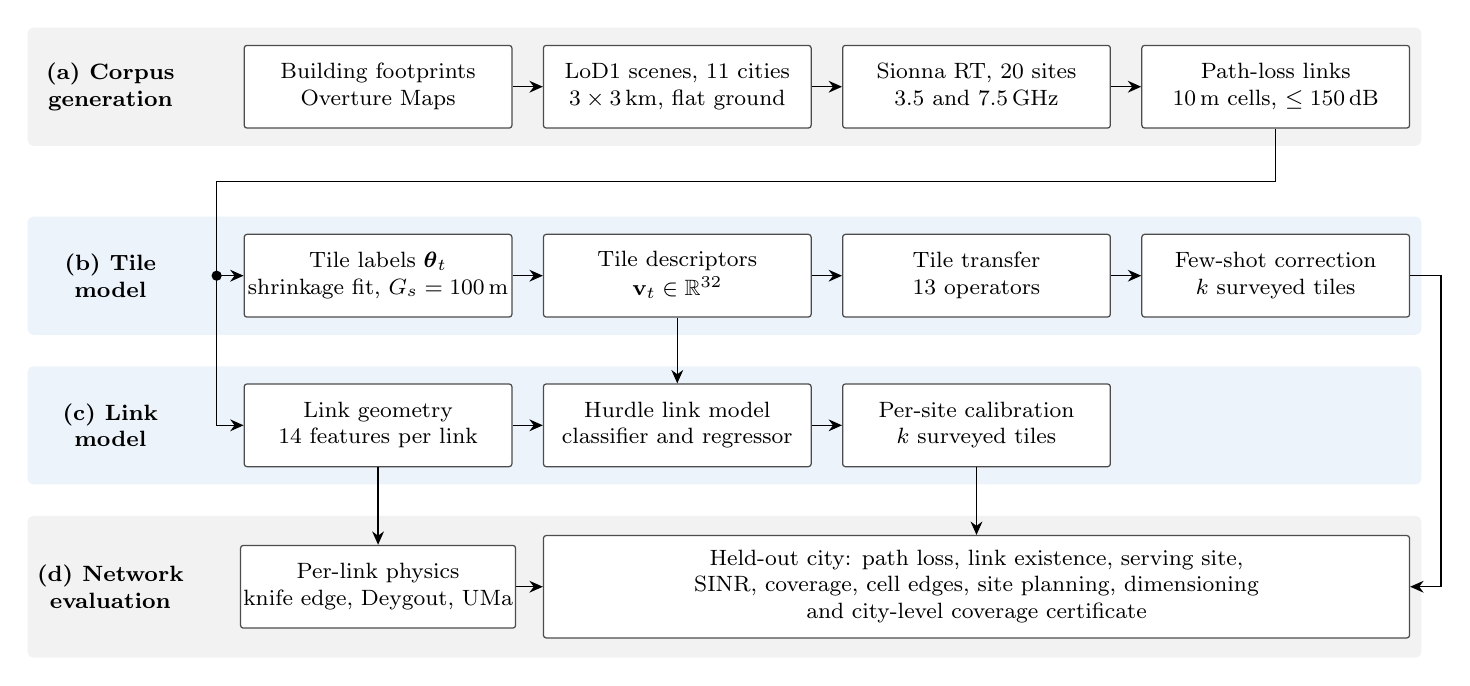
\begin{tikzpicture}[x=1mm, y=1mm, font=\footnotesize,
  box/.style={draw=black!70, fill=white, rounded corners=1pt, line width=0.45pt,
              minimum width=34mm, minimum height=10.5mm, align=center, inner sep=1pt},
  wide/.style={box, minimum width=110mm, minimum height=13mm},
  band/.style={rounded corners=2pt},
  lab/.style={font=\footnotesize\bfseries, align=center, anchor=center},
  arr/.style={-{Stealth[length=1.7mm, width=1.5mm]}, line width=0.5pt},
  dot/.style={circle, fill=black, inner sep=0pt, minimum size=1.3mm}]
\def\cA{44.5}\def\cB{82.5}\def\cC{120.5}\def\cD{158.5}
\def\rA{-7.5}\def\rB{-31.5}\def\rC{-50.5}\def\rD{-71}
\def\xR{177}\def\bus{24}
% ---- lanes
\fill[band, black!5]  (0,0)   rectangle (\xR,-15);
\fill[band, tnblue!9] (0,-24) rectangle (\xR,-39);
\fill[band, tnblue!9] (0,-43) rectangle (\xR,-58);
\fill[band, black!5]  (0,-62) rectangle (\xR,-80);
\node[lab] at (10.5,\rA) {(a) Corpus\\generation};
\node[lab] at (10.5,\rB) {(b) Tile\\model};
\node[lab] at (10.5,\rC) {(c) Link\\model};
\node[lab] at (10.5,\rD) {(d) Network\\evaluation};
% ---- (a) corpus generation
\node[box] (osm)   at (\cA,\rA) {\strut Building footprints\\\strut Overture Maps};
\node[box] (scene) at (\cB,\rA) {\strut LoD1 scenes, \nCities{} cities\\\strut $\sceneSize\times\sceneSize$\,km, flat ground};
\node[box] (rt)    at (\cC,\rA) {\strut Sionna RT, \nSitesPerCity{} sites\\\strut \freqGHz{} and \freqTwoGHz\,GHz};
\node[box] (links) at (\cD,\rA) {\strut Path-loss links\\\strut \cellSize\,m cells, $\le\maxPl$\,dB};
\draw[arr] (osm) -- (scene);
\draw[arr] (scene) -- (rt);
\draw[arr] (rt) -- (links);
% ---- (b) tile model
\node[box] (tile)  at (\cA,\rB) {\strut Tile labels $\boldsymbol{\theta}_t$\\\strut shrinkage fit, $G_s=\tileSize$\,m};
\node[box] (desc)  at (\cB,\rB) {\strut Tile descriptors\\\strut $\mathbf{v}_t\in\mathbb{R}^{32}$};
\node[box] (op)    at (\cC,\rB) {\strut Tile transfer\\\strut \nOps{} operators};
\node[box] (fs)    at (\cD,\rB) {\strut Few-shot correction\\\strut $k$ surveyed tiles};
\draw[arr] (tile) -- (desc);
\draw[arr] (desc) -- (op);
\draw[arr] (op) -- (fs);
% ---- (c) link model
\node[box] (feat)  at (\cA,\rC) {\strut Link geometry\\\strut 14 features per link};
\node[box] (hm)    at (\cB,\rC) {\strut Hurdle link model\\\strut classifier and regressor};
\node[box] (cal)   at (\cC,\rC) {\strut Per-site calibration\\\strut $k$ surveyed tiles};
\draw[arr] (feat) -- (hm);
\draw[arr] (hm) -- (cal);
\draw[arr] (desc) -- (hm);
% ---- (d) evaluation
\node[box] (phys)  at (\cA,\rD) {\strut Per-link physics\\\strut knife edge, Deygout, UMa};
\node[wide] (eval) at (\cC,\rD) {\strut Held-out city: path loss, link existence, serving site,\\\strut SINR, coverage, cell edges, site planning, dimensioning\\\strut and city-level coverage certificate};
\draw[arr] (feat) -- (phys);
\draw[arr] (phys) -- (eval);
\draw[arr] (cal) -- (cal |- eval.north);
\draw[arr] (fs.east) -- (\xR+2.5,\rB) -- (\xR+2.5,\rD) -- (eval.east);
% ---- links feed both lanes through one bus in the left margin
\draw[arr] (links.south) -- (\cD,-19.5) -- (\bus,-19.5) -- (\bus,\rB) -- (tile.west);
\draw[arr] (\bus,\rB) -- (\bus,\rC) -- (feat.west);
\node[dot] at (\bus,\rB) {};
\end{tikzpicture}

\caption{Processing pipeline. (a)~Geo-referenced scenes are built from
open building footprints and ray traced. (b)~Links are grouped into tiles; each tile
receives a label $\btheta_t=(\gamma_t,P_{L_0,t})$ and a descriptor
$\bv_t$ computed from the same scene geometry. (c)~Tile transfer operators
fitted on source cities predict the labels of a held-out city, optionally
corrected with $k$ surveyed tiles; the site-aware link model and the
per-link physics baselines predict every link from its geometry. All are
evaluated through the network quantities of Section~\ref{sec:netmodel}, a
site plan and a coverage certificate.}
\label{fig:pipeline}
\end{figure*}

\subsection{Ray-traced corpus}
\label{sec:corpus}

Each city is a square of side \SI{\sceneSize}{\kilo\metre} centred on a
fixed coordinate and expressed in a local metric frame, the UTM projection
of its zone shifted to the centre~\cite{snyder1987}. Building footprints are
taken from the buildings theme of Overture Maps~\cite{overture}, release
\overtureRelease{},
a versioned open dataset whose primary source is
OpenStreetMap~\cite{haklay2008osm}; a pinned release makes the geometry
exactly reproducible, which a live map query is not. Because grid north and
true north differ, the footprint query box covers all four corners of the
square. Building heights are resolved in order from the height attribute,
from the number of floors at \SI{3.2}{\metre} per floor, and otherwise from
the median of the resolved heights of the city; the share of each source is
reported per city. Footprint exteriors are clipped to the square, parts
smaller than \SI{4}{\metre\squared} are discarded, and the remainder is
extruded to level-of-detail~1 and placed on a flat ground plane. Buildings
use the ITU concrete model and the ground the ITU medium-dry-ground
model~\cite{itup2040}.

Each city has \nSitesPerCity{} sites on rooftops: local height maxima of
the building mesh on a \SI{25}{\metre} grid are ranked by height and
selected greedily with a minimum separation of \SI{\minSep}{\metre}, and the
antenna is mounted \SI{\siteMast}{\metre} above the roof; if too few
candidates satisfy the separation, the remaining sites are drawn at random
from the other rooftop candidates with a fixed seed. Ranking rooftops by
height follows macro-cell practice but places the sites of high-rise cities
on their tallest buildings: the median site height per city ranges from
\SI{\siteHMedMin}{\metre} (\siteHMedMinCity) to \SI{\siteHMedMax}{\metre}
(\siteHMedMaxCity), with a maximum of \SI{\siteHMax}{\metre} in
\siteHMaxCity{} (Table~\ref{tab:corpus}). Radio maps are
computed with Sionna~RT~\cite{hoydis2023sionna,hoydis2024learning}
(version~\sionnaVersion) at \SI{\freqGHz}{\giga\hertz} with isotropic
antennas, \rtSamples{} rays per site, maximum interaction depth
\rtDepth{}, specular and diffuse reflection, refraction and diffraction
(including edge diffraction) enabled, on a
\SI{\cellSize}{\metre} grid at \SI{\ueHeight}{\metre} receiver height. Cells
with path loss above $L_{\max}=\SI{\maxPl}{\decibel}$, beyond any practical
coupling loss, are discarded; a cell that no site reaches below $L_{\max}$
is a coverage hole of the truth and is kept as such in the evaluation. The
solver version and settings are stored with every city. \nSitesWord{} sites
on \SI{\sceneArea}{\kilo\metre\squared} give one site per
\SI{\areaPerSite}{\kilo\metre\squared}, the density of a hexagonal layout
with an inter-site distance of about \SI{\isdMain}{\metre}, sparser than the
\SI{500}{\metre} of the 3GPP urban-macro scenario~\cite{tr38901}. The
density and the siting rule are tested in Section~\ref{sec:res-robust}.

Four further corpora use the same scenes. The \emph{second band} re-traces
every site at \SI{\freqTwoGHz}{\giga\hertz}, in the \SIrange{7}{24}{\giga\hertz}
range studied for 6G~\cite{tr38820}. The \emph{random-siting replicate}
re-traces \nRandCities{} cities (\randCities) at \SI{\freqGHz}{\giga\hertz}
with the same number of sites taken from the rooftop candidates in random
order instead of by height, under the same separation rule; the
\emph{mid-rise replicate} draws them in random order from the rooftops
between \SI{\cappedLo}{\metre} and \SI{\cappedHi}{\metre} above ground, the
site-height range of the 3GPP urban-macro scenario; and the \emph{materials
replicate} keeps the main siting but assigns each building part one of
\nMat{} ITU materials (\matList) at random with a fixed seed instead of
concrete for all. The geometry, and hence every descriptor and link
feature, is identical across these replicates; only the ray-traced truth
changes.

\paragraph{Consistency check}
The planar radio-map estimator of the solver weights a ray crossing the
measurement plane by the inverse cosine of its incidence angle, and a
diffracted ray by an integration weight over the diffraction cone; the
first weight is unbounded and the second can be very large, so a cell
occasionally receives one overweighted contribution. Its path loss can then
fall below free space by tens of decibels, which no incoherent sum of a few
propagation paths allows. We remove every link whose path loss lies more
than \SI{\qcMargin}{\decibel} below the free-space loss at its 3-D distance:
\qcRemoved{} links, \qcShare\% of the corpus. For the site with the most
such links, disabling diffraction reduces the links more than
\SI{\qcMargin}{\decibel} below free space from \outDiffOn{} to \outDiffOff{}
with otherwise identical settings, which identifies the diffraction weights
as their source.

\subsection{Tile labels}
\label{sec:labels}

Links are assigned to tiles of side $G_s=\SI{\tileSize}{\metre}$ by their
receiver position; tiles with fewer than \minLinks{} links are not labelled.
Inside a tile, the ordinary least-squares (OLS) slope is poorly determined
because every receiver sees the serving sites from a similar distance: for
$\mathbf{A}=[\mathbf{x}\;\mathbf{1}]$ with $n$ rows,
$\det(\mathbf{A}^{\top}\mathbf{A})=n^{2}\Var(x)$ and
$\Var(\hat\gamma_{\mathrm{OLS}})=\sigma_\varepsilon^{2}/(n\Var(x))$, which
diverges as the intra-tile spread of $x$ vanishes. A receiver at distance
$d$ from its site sees a tile of side $G_s$ span only
$\Delta x\approx10\log_{10}(1+G_s/d)$, which is \SI{0.41}{\decibel} for
$G_s=\SI{100}{\metre}$ and $d=\SI{1}{\kilo\metre}$. We therefore shrink the
slope towards the city-wide mean with weights set by the data (empirical
Bayes~\cite{morris1983}).

\begin{proposition}[Empirical-Bayes shrinkage]
\label{prop:eb}
Let $b_t$ be the OLS slope of tile $t$, computed with $x$ centred inside
the tile, with sampling variance $v_t$, and let the true slopes vary between
tiles with mean $\mu$ and variance $\tau^{2}$. Among
estimators $\hat\gamma_t=(1-w)b_t+w\mu$ the mean squared error
$(1-w)^{2}v_t+w^{2}\tau^{2}$ is minimised by
\begin{equation}
w_t=\frac{v_t}{v_t+\tau^{2}}=\frac{\lambda_t}{\lambda_t+S_{xx,t}},
\qquad \lambda_t=\frac{S_{xx,t}\,v_t}{\tau^{2}},
\label{eq:eb}
\end{equation}
which is ridge regression on the centred slope with penalty $\lambda_t$
and prior mean $\mu$. Its risk is $v_t\tau^{2}/(v_t+\tau^{2})\le\min(v_t,\tau^{2})$,
bounded by $\tau^{2}$ however degenerate the tile geometry.
\end{proposition}

\noindent Radio-map cells served by the same site share propagation paths,
so the independent-residual variance $s_t^{2}/S_{xx,t}$ understates $v_t$.
We therefore use the cluster-robust variance of Eq.~\eqref{eq:cr} (below)
of the OLS slope, with the serving sites as clusters, never below the
independent value; a tile served by a single site uses the independent
value multiplied by the median ratio of the two over the city (its design
effect). We estimate $(\mu,\tau^{2})$ per city with the
DerSimonian--Laird moment estimator~\cite{dersimonian1986} over the tiles
with a non-degenerate span, set
$\hat\gamma_t=(1-w_t)b_t+w_t\hat\mu$, and leave the intercept unpenalised:
$\hat P_{L_0,t}=\bar y_t-\hat\gamma_t\bar x_t$. A tile with no span takes
$\hat\gamma_t=\hat\mu$. The shrinkage weight $w_t$ is published with every
label. Algorithm~\ref{alg:labels} states the procedure; it is vectorised
over all links of a city.

\begin{algorithm}[!t]
\SetAlgoLined\DontPrintSemicolon
\KwIn{links $(x_i,y_i,t_i,b_i)$ of one city; minimum count $n_{\min}$}
\KwOut{$\hat\btheta_t$, $w_t$, iid and cluster-robust standard errors}
\ForEach{tile $t$ with $n_t\ge n_{\min}$}{
  $\bar x_t,\bar y_t,S_{xx,t},S_{xy,t}$;\quad $b_t\leftarrow S_{xy,t}/S_{xx,t}$;\quad
  $v_t\leftarrow$ cluster-robust variance of $b_t$ (Eq.~\eqref{eq:cr})\;
}
$(\hat\mu,\hat\tau^{2})\leftarrow$ DerSimonian--Laird over $\{(b_t,v_t)\}$\;
\ForEach{tile $t$}{
  $w_t\leftarrow v_t/(v_t+\hat\tau^{2})$;\quad
  $\hat\gamma_t\leftarrow(1-w_t)b_t+w_t\hat\mu$;\quad
  $\hat P_{L_0,t}\leftarrow\bar y_t-\hat\gamma_t\bar x_t$\;
  residuals $e_i\leftarrow y_i-\hat P_{L_0,t}-\hat\gamma_t x_i$\;
  standard errors from Eq.~\eqref{eq:cr} with iid and with site clusters\;
}
\caption{Tile labels}
\label{alg:labels}
\end{algorithm}

\paragraph{Label precision}
The estimator is linear in the path losses. In the centred parametrisation
$y_i=a_t+\gamma_t(x_i-\bar x_t)+e_i$ with design rows
$\mathbf{z}_i=(1,x_i-\bar x_t)$, the coefficients are
$\mathbf{M}\sum_i\mathbf{z}_i y_i$ up to the prior term, with
$\mathbf{M}=\operatorname{diag}\bigl(1/n,\,1/(S_{xx,t}+\lambda_t)\bigr)$
($\lambda_t=0$ for the OLS slope), and $\hat P_{L_0,t}=\hat a_t-\hat\gamma_t\bar x_t$.
With the links of the tile partitioned by serving site into $G$ clusters
$\mathcal{I}_1,\dots,\mathcal{I}_G$, with design blocks $\mathbf{Z}_c$ and
residuals $\mathbf{e}_c$, the cluster-robust variance is
\begin{equation}
\widehat{\Var}_{\mathrm{cl}}=\mathbf{M}\Bigl(\sum_{c=1}^{G}\mathbf{u}_c\mathbf{u}_c^{\top}\Bigr)\mathbf{M},
\quad
\mathbf{u}_c=\mathbf{Z}_c^{\top}(\mathbf{I}-\mathbf{H}_{cc})^{-1/2}\mathbf{e}_c,
\label{eq:cr}
\end{equation}
with $\mathbf{H}_{cc}=\mathbf{Z}_c\mathbf{M}\mathbf{Z}_c^{\top}$ (Moore--Penrose
inverse root where $\mathbf{I}-\mathbf{H}_{cc}$ is singular). This is the
bias-reduced linearisation (CR2) of~\cite{bell2002,pustejovsky2018}; without
the factor $(\mathbf{I}-\mathbf{H}_{cc})^{-1/2}$ it is the usual
estimator~\cite{liang1986,cameron2015}, which is biased downwards when the
clusters are few, as here. Since
$\mathbf{Z}_c^{\top}f(\mathbf{Z}_c\mathbf{M}\mathbf{Z}_c^{\top})=f(\mathbf{Z}_c^{\top}\mathbf{Z}_c\mathbf{M})\mathbf{Z}_c^{\top}$
for $f(s)=(1-s)^{-1/2}$, every $\mathbf{u}_c$ requires only the eigen-decomposition
of a $2\times2$ matrix. The iid variance is
$s^{2}\,\mathbf{M}(\sum_i\mathbf{z}_i\mathbf{z}_i^{\top})\mathbf{M}$.
Because the number of clusters per tile is small,
Eq.~\eqref{eq:cr} is complemented by a split-half estimate: the sites of a
city are divided at random into two disjoint halves, the complete
estimator (including its own $\hat\mu,\hat\tau^2$) is refitted on each half,
and $\operatorname{sd}(\hat\gamma^{(1)}-\hat\gamma^{(2)})/\sqrt2$ estimates the
standard error of a half-data label; dividing by a further $\sqrt2$
extrapolates to the full data under the assumption that the variance scales
with the inverse number of sites. Five random partitions are pooled.

\subsection{Tile descriptors}
\label{sec:descriptors}

The descriptor must describe exactly the geometry the ray tracer saw. It is
therefore computed from the same footprint parts, heights and scene clipping
as the extruded mesh, with every part clipped to the tile it falls in. It
contains the $32$ built-environment features of~\cite{ozyurt2026}: footprint
ratio and building count in five height classes ($<5$, $5$--$10$,
$10$--$30$, $30$--$60$, $\ge\SI{60}{\metre}$); mean and standard deviation of
footprint area, height and volume; total footprint density; and, for
horizontal planes at $5$, $10$, $30$, $60$ and \SI{100}{\metre}, the number
of buildings reaching the plane and the mean and standard deviation of the
distance between their centroids. The topographic, land-cover and climatic
descriptors of~\cite{ozyurt2026} are omitted on purpose: the scenes have a
flat ground, no water or vegetation surfaces and no weather, so these
features would describe nothing the solver modelled and could only act as
city identifiers. Descriptors are stored unnormalised; every fit scales them
by the column-wise maximum absolute value of its own training tiles, never
of the target.

\subsection{Transfer operators}
\label{sec:operators}

We compare constant predictors, label-averaging operators and learned
regressors.
\begin{itemize}
\item \emph{Source median}: the median source label, the no-information
reference.
\item \emph{3GPP UMa}: the line-of-sight and non-line-of-sight single-slope
formulas of TR~38.901~\cite{tr38901} at the reference distance, which give
fixed parameters for every tile, and \emph{COST-231 Hata}~\cite{cost231}
(metropolitan correction, median site height of the source cities), used
outside its validity range of \SIrange{1.5}{2}{\giga\hertz} and
\SIrange{1}{20}{\kilo\metre} as a further standard model.
\item \emph{Kernel (Nadaraya--Watson)}~\cite{nadaraya1964,watson1964}, the
operator of~\cite{ozyurt2026}:
\begin{equation}
\hat\btheta_u=\sum_j\tilde w_j(u)\btheta_j,\qquad
\tilde w_j(u)\propto\exp\!\Bigl(-\frac{\lVert\bv_u-\bv_j\rVert^{2}}{2\sigma^{2}}\Bigr),
\label{eq:nw}
\end{equation}
computed with the minimum squared distance subtracted in the exponent, which
leaves the weights unchanged and avoids numerical underflow.
\item \emph{GP-ARD}: a Gaussian process with one length scale per
descriptor (automatic relevance determination)~\cite{rasmussen2006}, i.e.\ a
kernel operator whose metric is learned; the hyper-parameters maximise the
marginal likelihood on \num{600} random source tiles and the posterior mean
uses every source tile.
\item \emph{$k$-NN}: the mean label of the $k$ nearest source tiles.
\item \emph{Ridge}, a two-layer \emph{MLP}, gradient-boosted trees
(\emph{GBDT}, LightGBM~\cite{ke2017lightgbm}) and a \emph{neural encoder}
with a constrained $(\gamma,P_{L_0})$ head trained with a heteroscedastic
Gaussian likelihood.
\item Two domain-adaptation variants that use the unlabelled descriptors of
the target city: \emph{GBDT-IW} weights the source tiles by the density
ratio of target to source descriptors estimated with a logistic domain
classifier, clipped at its 99th percentile~\cite{shimodaira2000}, and
\emph{CORAL} re-colours the source descriptors with the target covariance
before ridge regression~\cite{sun2016coral}.
\end{itemize}

\paragraph{Nested selection}
Every hyper-parameter (bandwidth $\sigma$, $k$, ridge, CORAL and MLP
penalties, number of boosting rounds, number of epochs) is chosen inside the
training cities by an inner leave-one-training-city-out loop: each training
city is held out once, the operator is fitted on the others and scored by the
root-mean-square standardised error over both parameters, and the grid value
with the smallest mean inner error is kept. The operator is then refitted on
all training cities; for the operators with early stopping, the number of
rounds or epochs of the final fit is the median best iteration over the
inner folds. The two expensive operators, the neural encoder and the link
model of Section~\ref{sec:link}, use \nInnerExpensive{} inner validation
cities drawn with a fixed seed. No city is ever reserved for validation, so
the procedure is symmetric in the source cities, which the certificate of
Section~\ref{sec:neteval} requires, and the held-out city is never touched.
The chosen values are listed in Table~\ref{tab:hparams}. Stochastic
operators are run with five seeds; the inner selection uses seed 0.

\paragraph{Behaviour of kernel transfer}
Write $d_j=\lVert\bv_u-\bv_j\rVert^{2}$, $\delta_j=d_j-\min_k d_k\in[0,D_u]$,
$\bar\btheta=N^{-1}\sum_j\btheta_j$ and
$\sigma_\theta^{2}=N^{-1}\sum_j\lVert\btheta_j-\bar\btheta\rVert^{2}$.

\begin{proposition}[Two regimes of kernel transfer]
\label{prop:regimes}
(a)~If $\epsilon_u=D_u/(2\sigma^{2})<1$, then
\begin{equation}
\hat\btheta_u=\bar\btheta-\frac{1}{2\sigma^{2}}\Cov_j(\delta_j,\btheta_j)+O(\epsilon_u^{2}),\quad
\bigl\lVert\hat\btheta_u-\bar\btheta\bigr\rVert\le
\frac{D_u\,\sigma_\theta}{4\sigma^{2}}+O(\epsilon_u^{2}),
\label{eq:flat}
\end{equation}
and $n_{\mathrm{eff}}(u)=N(1+O(\epsilon_u^{2}))$: the operator returns the
source mean up to a first-order correction.
(b)~Let $g_u$ be the gap between the smallest and second-smallest squared
distance. Then the weight of the nearest source tile satisfies
\begin{equation}
\tilde w_{(1)}\ge\bigl(1+(N-1)e^{-g_u/(2\sigma^{2})}\bigr)^{-1},
\label{eq:nn}
\end{equation}
so $\hat\btheta_u$ tends to the label of the nearest source tile when
$g_u\gg2\sigma^{2}\ln N$.
\end{proposition}

\noindent The minimum distance cancels from Eq.~\eqref{eq:nw}; a target
far from every source tile is therefore \emph{not} by itself pushed to
either regime. Which regime applies is decided by the selected bandwidth
relative to the spread $D_u$ and the gap $g_u$, and we measure it
(Section~\ref{sec:res-kernel}) rather than assume it. Both regimes carry a
failure mode under shift: the flat regime returns the source mean and
ignores the target descriptor; the nearest-neighbour regime copies one
source tile and transmits its label noise undamped
(Eq.~\eqref{eq:decomp} with $n_{\mathrm{eff}}=1$).

\subsection{Few-shot correction}
\label{sec:fewshot}

With $k$ target tiles surveyed, the zero-shot prediction $g(\bv)$ is
corrected by the residuals $r_i=\btheta_i-g(\bv_i)$ of the $k$ anchors.
The anchors' labels are noisy (Section~\ref{sec:res-labels}), so the
correction weights each anchor by its precision and shrinks the result by
empirical Bayes, per parameter:
\begin{equation}
w_i=\frac{1}{\mathrm{se}_i^{2}+s^{2}},\quad
c=\frac{\sum_i w_i r_i}{\sum_i w_i},\quad
V=\frac{1}{\sum_i w_i},\quad
c_{\mathrm{EB}}=\frac{\tau_b^{2}}{\tau_b^{2}+V}\,c,
\label{eq:fewshot}
\end{equation}
with $\mathrm{se}_i$ the cluster-robust standard error of the anchor label,
$s^{2}$ the within-city error variance of the operator and $\tau_b^{2}$ the
between-city variance of its zero-shot bias, both estimated on the inner
validation cities of the fold (no target information). When the inner
cities show no systematic bias, $\tau_b^{2}\to0$ and the correction
vanishes; when they do, the correction is the precision-weighted mean
residual. We compare it with the plain mean residual (\emph{bias}) and with a
precision-weighted ridge model of the residual on the descriptors
(\emph{residual}, penalty $10$ on normalised descriptors). Anchors are drawn
uniformly at random, as the $k$ tiles closest to a random tile
(\emph{contiguous}), which mimics a single drive-test
area~\cite{johansson2012mdt}, or by a \emph{design} that uses no
measurement: the $k$ tiles that greedily maximise the facility-location
objective $\sum_{i}\max_{j\in T}\exp(-\lVert\bv_i-\bv_j\rVert^{2}/2h^{2})$
over the target tiles, with $h$ the median pairwise descriptor distance; the
objective is monotone submodular, so the greedy set is within a factor
$(1-1/e)$ of the optimum~\cite{nemhauser1978,krause2008}. Evaluation is
always on the unsurveyed tiles, anchors are shared by all operators, and
ten random draws are made per $k\in\{3,5,10,25,50,100\}$.

\subsection{Site-aware link transfer and per-link baselines}
\label{sec:link}

As a transfer model free of the receiver-tile restrictions we predict the
path loss of each (pixel, site) link directly. The features are computed
from the scene geometry only, so they are available for a city without any
measurement. The building heights are rasterised at \SI{2}{\metre} and the
straight segment from the site to the pixel is sampled at $96$ interior
points, where the building height $H(s)$ is compared with the
line-of-sight height $h_{\mathrm{los}}(s)$. The link features are the 3-D and
horizontal distances, the site height and the elevation angle; the fraction
of the segment with $H>h_{\mathrm{los}}$, the number of separate
obstructions and the length over footprints; the largest excess height
$\max_s(H-h_{\mathrm{los}})$; the single knife-edge loss
$J(\nu)=6.9+20\log_{10}\bigl(\sqrt{(\nu-0.1)^{2}+1}+\nu-0.1\bigr)$ for
$\nu>-0.78$ (zero otherwise) of the most obstructing point, with
$\nu=h\sqrt{2(1/d_1+1/d_2)/\lambda}$~\cite{itup526}; whether the receiver lies
inside a footprint and that building's height; and the built fraction and
mean building height in a \SI{100}{\metre} square window centred on the
receiver and the built fraction in a \SI{200}{\metre} window centred on the
site. The $32$ descriptors of the receiver's
tile are appended.

The ray tracer reports only links below the cut-off, so a regressor trained
on them never learns that a distant, obstructed site is not received at all;
it would predict a finite loss for every link and overstate the reach of
every site. We therefore use a hurdle model: a gradient-boosted
classifier~\cite{ke2017lightgbm} of whether a (pixel, site) pair lies below
the cut-off, trained on \num{120000} pairs of each training city (all sites
and the pixels of its labelled tiles, including the pairs beyond the
cut-off), and a gradient-boosted regressor of the path loss, trained on
\num{120000} ray-traced links of each training city. A link is predicted
beyond the cut-off (zero received power) when the classifier gives a
probability below one half, and otherwise its path loss is the regression.
The number of rounds of both models follows the nested rule of
Section~\ref{sec:operators} (learning rate $0.1$, $127$ leaves, at most
$1500$ rounds, five seeds). The path-loss error of the link model is that of
the regressor over the ray-traced links; the regressor alone, which keeps
every link, is reported as an ablation, and a censored error that scores
every pair with prediction and truth clipped at $L_{\max}$ is reported as
well.

\paragraph{Per-link physics baselines}
Three non-learned predictors use the same link geometry and the
deterministic hurdle ``predicted loss $\le L_{\max}$'': free space plus the
single knife-edge loss $J(\nu)$ above; free space plus the Deygout
three-edge construction of ITU-R P.526~\cite{itup526} (the principal edge
and the largest edge on each sub-path); and the 3GPP UMa model of
TR~38.901~\cite{tr38901} with the line-of-sight state of each link decided
from the geometry, its breakpoint, and
$P_{L,\mathrm{NLOS}}=\max(P_{L,\mathrm{LOS}},P'_{L,\mathrm{NLOS}})$. They
answer the question whether a learned link model is needed at all once the
obstruction geometry is available.

\paragraph{Receiver-tile variants}
To attribute the gap between the tile model and link transfer, every tile
operator is also evaluated (i)~with the hurdle of the link model applied to
its map (seed-matched), (ii)~as a dual-slope model with one
$(\gamma,P_{L_0})$ pair per tile fitted to the line-of-sight links and one
to the obstructed links, the state of each (pixel, site) pair decided from
the geometry, each pair falling back to the all-link label where fewer than
\minLinks{} links of its kind exist, and (iii)~with both. GBDT transfers
the four labels of the dual-slope model under the nested rule.

\paragraph{Survey design for site calibration}
In the few-shot variant the links observed in $k$ surveyed tiles, which carry
their serving site as minimisation-of-drive-tests (MDT) reports
do~\cite{johansson2012mdt,ts37320}, calibrate a per-site offset. Model the
residual of a link of site $s$ as $o_s+\varepsilon$, with independent site
offsets $o_s$ of prior mean $\bar o$ and variance $\tau_o^{2}$ and link noise of
variance $\sigma_\varepsilon^{2}$, and let $\kappa=\sigma_\varepsilon^{2}/\tau_o^{2}$.
With $n_s$ observed links of site $s$ and mean residual $\bar r_s$, the
posterior mean of $o_s$ is $(n_s\bar r_s+\kappa\bar o)/(n_s+\kappa)$, which we
use with $\bar o$ the mean residual of all observed links; $\kappa$ is
estimated from the surveyed links themselves by the DerSimonian--Laird
moment estimator over the site means (empirical Bayes), so that a survey
whose site means scatter no more than their sampling error applies the
overall offset only, and a fixed $\kappa=\kappaLink{}$ links is reported as
an ablation. The posterior variance of $o_s$ is $\tau_o^{2}\kappa/(n_s+\kappa)$.

\begin{proposition}[Survey design]
\label{prop:survey}
Let $c_{ts}\ge0$ be the number of links of site $s$ observable in tile $t$
and $n_s(T)=\sum_{t\in T}c_{ts}$ for a set $T$ of surveyed tiles. The total
reduction of posterior variance of the site offsets,
\begin{equation}
F(T)=\tau_o^{2}\sum_{s}\frac{n_s(T)}{n_s(T)+\kappa},
\label{eq:survey}
\end{equation}
is monotone and submodular in $T$, so the greedy choice of $k$ tiles attains
$F(T_{\mathrm{greedy}})\ge(1-1/e)\max_{|T|=k}F(T)$.
\end{proposition}

\noindent Before any measurement $c_{ts}$ is unknown; the \emph{variance
design} uses the number of links of site $s$ in tile $t$ that the hurdle
classifier of the zero-shot link model predicts below the cut-off. Because
maximising $F$ alone favours tiles that see many sites, which need not be
representative of the city, a \emph{stratified design} first partitions the
tiles into $k$ descriptor strata ($k$-means) and takes in each stratum the
tile with the largest marginal gain of $F$. Both are compared with random
surveys for $k\in\{10,25,50\}$ (ten draws). The surveyed pixels keep their
model prediction, and every few-shot metric is computed on the unsurveyed
pixels only.

\subsection{Network-level evaluation}
\label{sec:neteval}

For the held-out city, each operator's tile parameters and the true site
positions define a predicted path-loss map for every (pixel, site) pair
through Eq.~\eqref{eq:logdist}; the ray-traced map is the truth over every
cell of the solver grid inside a labelled tile, with pairs beyond the
cut-off treated as zero received power and cells no site reaches as outage
pixels (\unreachedShare\% of the pixels, \unreachedMin--\unreachedMax\%
across cities). With $P_{\mathrm{tx}}=\SI{46}{dBm}$, \SI{20}{\mega\hertz}
bandwidth and a \SI{7}{\decibel} noise figure ($N=\SI{-94.0}{dBm}$) we
compute the path-loss error over all ray-traced links, the censored error
over all pairs, the precision and recall of the predicted link existence,
the serving site over the pixels the truth reaches (a pixel a predictor does
not reach counts as wrong), coverage at $L\in\{120,130,140\}$\,dB, the SINR
of Eq.~\eqref{eq:sinr} and the spectral efficiency (attenuated Shannon,
factor $0.6$, zero below \SI{-10}{\decibel}, capped at
\SI{4.4}{b/s/Hz}~\cite{tr36942}). An SINR below \SI{\sinrFloor}{\decibel},
including a pixel at which no site is predicted to be received, is set to
\SI{\sinrFloor}{\decibel} (outage) for the truth and every predictor alike.
Mobility decisions depend on where the serving cell changes: a pixel is a
cell-edge pixel when its eastern or northern neighbour has a different
serving site (one pixel per boundary crossing), the \emph{edge displacement}
is the mean distance between the true and the predicted cell edges (the
average of the two directed mean nearest-edge distances), and the
\emph{edge-length error} is the relative error of the number of cell-edge
pixels, a proxy for the handover rate along a route.

\paragraph{Site planning}
Selecting $K$ of the $|\mathcal{B}|$ sites to maximise the number of covered
pixels is a monotone submodular maximisation, for which the greedy algorithm
attains a $(1-1/e)$ approximation of the optimum of the function it is
given~\cite{nemhauser1978}; site selection with propagation models is a
classical planning task~\cite{amaldi2003}. We run the greedy on the
\emph{predicted} coverage at \SI{140}{\decibel} and score the selected sites
on the \emph{true} coverage. The regret is the true coverage of the greedy
plan computed on the true map minus that of the plan computed on the
predicted map. For dimensioning, we also count the sites that the greedy
order on the predicted map needs to cover \covTarget\% of the pixels, and
the true coverage those sites achieve.

\paragraph{Certified coverage}
A planner must decide which pixels to \emph{promise} as covered. For a
transfer model and a held-out city $c$, let
$r_p=\min\{PL_{\mathrm{serv}}(p),C\}-\widehat{PL}_{\mathrm{serv}}(p)$ be the
true serving path loss of pixel $p$ (the smallest path loss over the sites),
censored at the cut-off $C=\SI{\maxPl}{\decibel}$ of the corpus, minus the
predicted one, and $q_c$ the $(1-\alpha)$ quantile of $\{r_p\}$ over the
pixels of $c$. The censoring keeps $q_c$ finite in a city where more than a
fraction $\alpha$ of the pixels is reached by no site; where the model itself
predicts no reaching site, $r_p=-\infty$ and the pixel is never claimed.

\begin{proposition}[City-level coverage certificate]
\label{prop:certify}
Let the $n$ cities be exchangeable and the training procedure symmetric in
its source cities. With $q_c$ computed from the leave-one-city-out model of
each city $c$, let $\hat q_t$ be the $j$-th largest of $\{q_c\}_{c\ne t}$ for
a target city $t$, and claim pixel $p$ as covered at level $L<C$ when
$\widehat{PL}_{\mathrm{serv}}(p)+\hat q_t\le L$. Then, with probability at
least $(n-j)/n$ over the draw of the target city, at most a fraction
$\alpha$ of its pixels are claimed but not covered.
\end{proposition}

\noindent The guarantee is at the level of cities, the unit of shift, in the
spirit of conformal prediction~\cite{vovk2005,barber2021}; it needs no model
of the residuals, and the nested selection of Section~\ref{sec:operators}
provides the required symmetry. The rank $j$ trades confidence for
coverage: $j=1$ (the largest margin of the other cities) gives probability
$(n-1)/n$, $j=2$ gives $(n-2)/n$ with a smaller margin. We report it at
$L=\SI{140}{\decibel}$ for $\alpha\in\{0.05,0.10\}$ and $j\in\{1,2\}$ (the
results at \SI{130}{\decibel} are released with the code) with the claimed
and the falsely claimed share of the pixels, and compare it with the naive
claim $\widehat{PL}_{\mathrm{serv}}(p)\le L$.

\subsection{Robustness analyses}
\label{sec:robust}

\emph{Mixed-path composition.} The framework of~\cite{ozyurt2026}, following
MAPLE~\cite{ozyurt2020maple}, composes the loss of a link from every tile
its straight path crosses. We split the horizontal segment from each site to
each pixel at the tile borders (sampled every \SI{10}{\metre}), so that tile
$t$ holds a length $L_t$ of it, between the distances $d_t^{\mathrm{in}}$
and $d_t^{\mathrm{out}}$ from the site, and evaluate two readings of the
composition as a propagation law. The \emph{piecewise} reading is a
multi-slope law along the path,
$\PL=A_{s}+\sum_t 10\gamma_t\log_{10}\big(\max(d_t^{\mathrm{out}},d_0)/
\max(d_t^{\mathrm{in}},d_0)\big)$, with the intercept of the site's tile $s$
and, over each stretch of distance, the exponent of the tile it lies in. The
\emph{path-averaged} reading averages the parameters along the path,
$\PL=\sum_t (L_t/d_h)\,[A_t+\gamma_t x]$ with the horizontal length $d_h$.
Both reduce to Eq.~\eqref{eq:logdist} when the whole path lies in one tile.
A third, literal reading that sums one log-distance loss per crossed tile is
reported in \ref{app:summed}. All are linear in the tile parameters, which
are fitted jointly to all links of a city by least squares with a weak ridge
penalty ($\lambda=10$) towards the best city-wide pair; they are evaluated
with tiles of \SI{100}{\metre} and, as in~\cite{ozyurt2026}, of
\SI{200}{\metre}, \SI{500}{\metre} and \SI{1000}{\metre}, always on the
pixels of the main corpus. The labels of the tiles crossed by at least 30
links are transferred with the source median, kernel transfer and GBDT under
the protocol of Section~\ref{sec:protocol} (one seed), and the predicted
maps are scored as in Section~\ref{sec:neteval}.
\emph{Network size.} Every zero-shot predictor is also scored on the network
of the first ten sites selected by the siting rule (one site per
\SI{0.9}{\kilo\metre\squared}, inter-site distance about
\SI{\isdSmall}{\metre}). \emph{Siting and materials.} The models trained
on the main corpus are applied unchanged to the three replicates; the tile
model is scored with labels fitted on the replicate itself and with the
labels of the same tiles from the main corpus. \emph{Tile size.} Labels,
descriptors, zero-shot transfer (median, ridge, GBDT) and the network
evaluation are repeated for $G_s\in\{50,100,200\}$\,m. \emph{Censoring.}
Links beyond the cut-off are missing, which can bias a least-squares slope.
We refit the labels with the cut lowered to $140$ and \SI{130}{\decibel}
and, for \num{300} random tiles per city, compare the least-squares slope
with that of a censored-Gaussian (Tobit) model~\cite{tobin1958} that also
uses the (pixel, site) pairs beyond the cut. \emph{Second band.} The tile
and link pipelines are repeated at \SI{\freqTwoGHz}{\giga\hertz}, and the
\SI{\freqGHz}{\giga\hertz} link models are applied to the second band with
the free-space offset $20\log_{10}(f_2/f_1)$, their knife-edge feature
evaluated at the new wavelength. \emph{External scenes.} The Munich,
\'Etoile and Florence scenes distributed with Sionna~RT were modelled
independently of our corpus, with detailed meshes and several ITU materials
(brick, concrete, marble, metal, wood). We derive building footprints and
heights from their meshes by vertical ray casting on a \SI{2}{\metre} grid,
place \nExtSites{} rooftop sites per scene with the rule of our corpus
(minimum separation \SI{\extMinSep}{\metre}, the scenes being smaller), ray
trace them with the corpus settings and evaluate, without any retraining,
the tile labels, the source median, ridge and GBDT fitted on all eleven
cities under the nested rule, and the mean of the eleven leave-one-city-out
link models, zero-shot and with the per-site calibration of
Section~\ref{sec:link} from $k\in\{10,25\}$ surveyed tiles (ten random
draws, and the two designs), scored on the unsurveyed pixels. The San
Francisco scene has terrain and would require a terrain-following
measurement surface; it is not used.

\subsection{Protocol and inference}
\label{sec:protocol}

Every city is the target once (leave-one-city-out) and the other cities are
training cities, inside which the nested selection of
Section~\ref{sec:operators} takes place. Tiles of one city are spatially
correlated, so tile-level tests would overstate significance; the unit of
inference is the target city. For each comparison we report the mean
per-city difference, a 95\% percentile bootstrap interval over
cities~\cite{efron1993}, the exact two-sided Wilcoxon signed-rank
$p$-value~\cite{wilcoxon1945} and the number of cities in which the first
operator is better, with Holm's correction~\cite{holm1979} within each
family of comparisons. Standard deviations across cities use $n-1$. With
\nCities{} cities an exact Wilcoxon test can reach $p<0.05$ only when nearly
every city agrees; we state the power limit where it matters.
%
%% ===================================================================
\section{Results}
\label{sec:results}

\subsection{Corpus and ray-budget convergence}
\label{sec:res-corpus}

The corpus contains \nCities{} cities, \nBuildings{} buildings,
\nSites{} sites and \nSamples{} ray-traced links (Table~\ref{tab:corpus});
\nTiles{} tiles have at least \minLinks{} links and are labelled.
Figure~\ref{fig:city} shows one city. The share of buildings whose height
is imputed from the city median ranges from \impMin\% (\impMinCity) to
\impMax\% (\impMaxCity).

The radio-map solver is a Monte-Carlo method: a cell that no ray reaches
reports zero power, so the set of reached cells and their values depend on
the ray budget. Table~\ref{tab:convergence} compares budgets with a
reference run of \convRef{} rays for \convNSites{} sites in \convNCities{}
cities. At the \rtSamples{} rays per site used for the corpus, path loss
below \SI{120}{\decibel} agrees with the reference to at most
\SI{\convRmsOneTwentyMax}{\decibel} RMS and path loss below
\SI{140}{\decibel} to \convRmsOneFortyMin--\SI{\convRmsOneFortyMax}{\decibel},
with a mean difference of at most \SI{\convBiasOneFortyMax}{\decibel}; the
number of cells reached below \SI{140}{\decibel} is at least
\convCellsOneFortyMin\% of the reference, and below the cut-off at least
\convCellsOneFiftyMin\%. These figures are the noise floor of the truth:
a model cannot be expected to match the corpus more closely than
\SIrange{\convRmsOneFortyMin}{\convRmsOneFortyMax}{\decibel} near the
cut-off, and up to \convRmsOneFiftyMax{}\,dB for the faintest links. The
complete corpus took \rtHours{}\,h on a \rtBackend{} backend
(\rtSecPerSite{}\,s per site).

\begin{table*}[!t]
\centering
\caption{Corpus. Height source: share of buildings with an explicit height
attribute, with a floor count, or imputed from the city median. Site
height: antenna height above ground of the \nSitesPerCity{} sites. Links:
ray-traced (pixel, site) pairs below the \SI{\maxPl}{\decibel} cut-off.
Tiles: labelled tiles ($\ge\minLinks{}$ links).}
\label{tab:corpus}
\small
% generated by paper/scripts/make_assets.py
\begin{tabular}{lrrrrrrrrrr}
\toprule
& & \multicolumn{3}{c}{Height source (\%)} & & \multicolumn{3}{c}{Site height (m)} & & \\
\cmidrule(lr){3-5}\cmidrule(lr){7-9}
City & Buildings & tag & storeys & imputed & Median (m) & min & med. & max & Links & Tiles \\
\midrule
Amsterdam & 21{,}135 & 83 & 2 & 15 & 15.5 & 39 & 47 & 67 & 736{,}255 & 948 \\
Barcelona & 12{,}337 & 12 & 64 & 23 & 19.2 & 44 & 56 & 91 & 609{,}050 & 942 \\
Berlin & 6{,}036 & 15 & 63 & 22 & 16.0 & 44 & 75 & 374 & 1{,}009{,}619 & 957 \\
Chicago & 2{,}952 & 70 & 4 & 25 & 15.9 & 175 & 200 & 346 & 1{,}069{,}552 & 961 \\
Hamburg & 4{,}335 & 17 & 42 & 41 & 16.0 & 38 & 51 & 116 & 1{,}152{,}125 & 961 \\
London & 11{,}891 & 8 & 42 & 50 & 12.8 & 48 & 64 & 161 & 931{,}288 & 940 \\
Munich & 8{,}616 & 9 & 49 & 42 & 12.8 & 32 & 38 & 97 & 794{,}056 & 950 \\
New York & 7{,}126 & 98 & 1 & 2 & 18.6 & 232 & 318 & 478 & 827{,}510 & 960 \\
Paris & 14{,}383 & 3 & 64 & 33 & 19.2 & 38 & 46 & 96 & 529{,}649 & 910 \\
Prague & 9{,}907 & 1 & 70 & 29 & 16.0 & 38 & 41 & 222 & 783{,}805 & 960 \\
Vienna & 7{,}082 & 26 & 60 & 14 & 16.0 & 41 & 45 & 84 & 534{,}491 & 939 \\
\midrule
Total & 105{,}800 & & & & & & & & 8{,}977{,}400 & 10{,}428 \\
\bottomrule
\end{tabular}

\end{table*}

\begin{table*}[!t]
\centering
\caption{Ray-budget convergence (\SI{\cellSize}{\metre} cells). For each
path-loss level: number of cells reached below that level, relative to the
reference run (\%; Monte-Carlo noise can exceed 100\%), and RMS path-loss
difference to the reference over the cells reached by both (dB). s: solver
time.}
\label{tab:convergence}
\small
% generated by paper/scripts/make_assets.py
\begin{tabular}{rrrrrrrrrr}
\toprule
& & \multicolumn{2}{c}{$\le120$\,dB} & \multicolumn{2}{c}{$\le130$\,dB} & \multicolumn{2}{c}{$\le140$\,dB} & \multicolumn{2}{c}{$\le150$\,dB} \\
\cmidrule(lr){3-4}\cmidrule(lr){5-6}\cmidrule(lr){7-8}\cmidrule(lr){9-10}
Rays & s & cells & RMS & cells & RMS & cells & RMS & cells & RMS \\
\midrule
\multicolumn{10}{l}{\emph{Amsterdam, site 0.0, 67\,m; reference \num{1e9} rays}} \\
\num{1e7} & 5 & 96.2 & 1.69 & 82.3 & 2.89 & 74.2 & 4.48 & 73.0 & 6.73 \\
\num{3e7} & 15 & 99.9 & 0.98 & 92.5 & 1.88 & 86.3 & 3.05 & 83.8 & 4.50 \\
\num{1e8} & 47 & 100.5 & 0.50 & 98.2 & 1.08 & 94.7 & 1.93 & 92.4 & 3.04 \\
\num{3e8} & 142 & 100.2 & 0.29 & 99.7 & 0.68 & 98.6 & 1.21 & 97.4 & 1.93 \\
\num{1e9} & 464 & 100.0 & 0.00 & 100.0 & 0.00 & 100.0 & 0.00 & 100.0 & 0.00 \\
\multicolumn{10}{l}{\emph{Amsterdam, site 10.0, 46\,m; reference \num{1e9} rays}} \\
\num{1e7} & 5 & 94.4 & 1.55 & 83.0 & 2.74 & 67.4 & 4.36 & 64.5 & 6.57 \\
\num{3e7} & 14 & 98.4 & 0.92 & 92.4 & 1.97 & 79.4 & 3.28 & 75.6 & 5.24 \\
\num{1e8} & 43 & 98.8 & 0.80 & 97.5 & 1.38 & 89.2 & 2.35 & 85.7 & 3.81 \\
\num{3e8} & 125 & 98.9 & 0.63 & 100.3 & 1.11 & 96.9 & 1.81 & 94.9 & 2.81 \\
\num{1e9} & 422 & 100.0 & 0.00 & 100.0 & 0.00 & 100.0 & 0.00 & 100.0 & 0.00 \\
\multicolumn{10}{l}{\emph{New York, site 0.0, 478\,m; reference \num{1e9} rays}} \\
\num{1e7} & 5 & 99.4 & 0.96 & 95.2 & 1.73 & 80.4 & 2.99 & 77.2 & 4.54 \\
\num{3e7} & 11 & 99.9 & 0.74 & 99.6 & 1.20 & 90.8 & 2.24 & 89.4 & 3.45 \\
\num{1e8} & 36 & 99.7 & 0.61 & 100.0 & 0.87 & 95.9 & 1.69 & 96.5 & 2.49 \\
\num{3e8} & 109 & 99.8 & 0.50 & 100.0 & 0.66 & 98.5 & 1.34 & 99.0 & 1.89 \\
\num{1e9} & 362 & 100.0 & 0.00 & 100.0 & 0.00 & 100.0 & 0.00 & 100.0 & 0.00 \\
\multicolumn{10}{l}{\emph{New York, site 10.0, 311\,m; reference \num{1e9} rays}} \\
\num{1e7} & 5 & 98.0 & 1.33 & 93.6 & 2.01 & 86.5 & 3.14 & 82.6 & 4.48 \\
\num{3e7} & 15 & 99.0 & 0.87 & 96.9 & 1.32 & 93.5 & 2.16 & 91.3 & 3.22 \\
\num{1e8} & 48 & 99.7 & 0.63 & 98.9 & 0.95 & 97.7 & 1.55 & 96.9 & 2.23 \\
\num{3e8} & 146 & 99.7 & 0.42 & 99.7 & 0.65 & 99.4 & 1.02 & 99.2 & 1.47 \\
\num{1e9} & 478 & 100.0 & 0.00 & 100.0 & 0.00 & 100.0 & 0.00 & 100.0 & 0.00 \\
\multicolumn{10}{l}{\emph{Paris, site 0.0, 96\,m; reference \num{1e9} rays}} \\
\num{1e7} & 5 & 97.4 & 1.21 & 89.5 & 2.18 & 80.7 & 3.34 & 74.7 & 4.91 \\
\num{3e7} & 15 & 100.1 & 0.69 & 96.1 & 1.37 & 89.9 & 2.31 & 84.8 & 3.39 \\
\num{1e8} & 43 & 100.2 & 0.33 & 99.3 & 0.78 & 96.0 & 1.44 & 92.9 & 2.27 \\
\num{3e8} & 132 & 100.1 & 0.18 & 100.0 & 0.49 & 98.9 & 0.98 & 97.8 & 1.62 \\
\num{1e9} & 428 & 100.0 & 0.00 & 100.0 & 0.00 & 100.0 & 0.00 & 100.0 & 0.00 \\
\multicolumn{10}{l}{\emph{Paris, site 10.0, 45\,m; reference \num{1e9} rays}} \\
\num{1e7} & 5 & 92.0 & 1.72 & 77.6 & 3.01 & 70.8 & 4.64 & 70.6 & 6.77 \\
\num{3e7} & 14 & 97.0 & 1.17 & 87.8 & 2.35 & 82.2 & 3.79 & 81.3 & 5.40 \\
\num{1e8} & 50 & 99.5 & 0.78 & 96.9 & 1.68 & 93.0 & 2.68 & 91.3 & 3.61 \\
\num{3e8} & 149 & 100.3 & 0.55 & 99.4 & 1.18 & 97.5 & 1.79 & 97.0 & 2.39 \\
\num{1e9} & 461 & 100.0 & 0.00 & 100.0 & 0.00 & 100.0 & 0.00 & 100.0 & 0.00 \\
\bottomrule
\end{tabular}

\end{table*}

\begin{figure*}[!t]
\centering
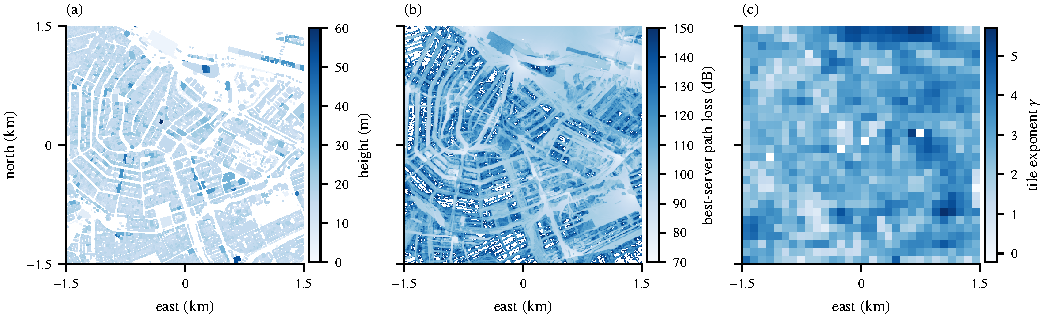
\includegraphics[width=\textwidth]{figures/fig_city.pdf}
\caption{\figCity{}. (a)~Building heights of the scene. (b)~Ray-traced path loss
to the best site. (c)~Tile exponents $\hat\gamma_t$.}
\label{fig:city}
\end{figure*}

\subsection{Tile labels and their precision}
\label{sec:res-labels}

Table~\ref{tab:fits} summarises the labels. City medians of the tile
exponent range from \gammaMedMin{} (\gammaMedMinCity) to \gammaMedMax{}
(\gammaMedMaxCity); their standard deviation across cities, \betweenSd, is
only \betweenWithinRatio{} times the typical standard deviation of the
tiles within a city (\withinSdMin--\withinSdMax). Most of the variation of
the tile exponent is therefore within cities, not between them. The fit
residual of the log-distance law inside a tile is
\fitRmseMin--\SI{\fitRmseMax}{\decibel}. The city-wide exponent of a single
law over all links is below the free-space value in \nCityGammaBelowTwo{}
cities (\cityGammaMinCity: \cityGammaMin), the joint effect of high sites
and of the censoring of far links (Section~\ref{sec:res-robust}); the tile
labels, fitted inside \SI{100}{\metre}, do not show this artefact.

Without shrinkage, the OLS exponents span \olsMin{} to \olsMax{}, the
ill-conditioning of Section~\ref{sec:labels}; empirical-Bayes shrinkage
(median weight \shrinkMedian) narrows this to \ebMin{} to \ebMax.
Label precision is the decisive quantity (Table~\ref{tab:noise}). The
standard error assuming independent residuals is \seIid; the
cluster-robust error with sites as clusters is \seCluster, \seRatio{} times
larger, and the split-half estimate extrapolated to the full data is
\seSplit. The exponent of a tile therefore depends strongly on which sites
serve it, and a label error of this size is comparable to the differences
between cities.

\begin{table*}[!t]
\centering
\caption{Tile labels per city. City-wide fit: OLS over all links. Tile labels:
median and standard deviation of $\hat\gamma_t$ and median $\hat P_{L_0,t}$
(dB, at $d_0=\SI{\refDist}{\metre}$); $\hat\tau$: between-tile standard deviation
of the slope; $w_t$: shrinkage weight; RMSE: link-weighted fit residual (dB).}
\label{tab:fits}
\small
% generated by paper/scripts/make_assets.py
\begin{tabular}{lrrrrrrrr}
\toprule
& \multicolumn{2}{c}{City-wide fit} & \multicolumn{3}{c}{Tile labels} & & & \\
\cmidrule(lr){2-3}\cmidrule(lr){4-6}
City & $\gamma$ & $P_{L_0}$ & med.\ $\gamma$ & s.d.\ $\gamma$ & med.\ $P_{L_0}$ & $\hat\tau$ & med.\ $w_t$ & RMSE \\
\midrule
Amsterdam & 2.47 & 100.5 & 2.84 & 0.93 & 100.9 & 1.06 & 0.27 & 11.3 \\
Barcelona & 1.92 & 105.4 & 2.43 & 0.96 & 105.5 & 1.14 & 0.28 & 11.6 \\
Berlin & 2.65 & 98.2 & 2.82 & 0.81 & 97.5 & 1.00 & 0.36 & 11.6 \\
Chicago & 0.81 & 115.6 & 2.79 & 0.83 & 97.2 & 1.19 & 0.54 & 12.7 \\
Hamburg & 2.14 & 100.2 & 3.15 & 0.72 & 92.2 & 0.94 & 0.37 & 11.4 \\
London & 1.72 & 104.4 & 2.40 & 0.60 & 103.3 & 0.79 & 0.42 & 11.2 \\
Munich & 2.12 & 104.0 & 3.00 & 0.80 & 99.8 & 0.92 & 0.33 & 11.2 \\
New York & 1.11 & 115.9 & 2.69 & 0.79 & 102.2 & 1.18 & 0.53 & 12.6 \\
Paris & 2.06 & 103.6 & 2.41 & 0.95 & 106.7 & 1.13 & 0.29 & 11.8 \\
Prague & 2.48 & 100.9 & 2.92 & 0.77 & 99.0 & 0.95 & 0.37 & 11.4 \\
Vienna & 2.29 & 106.1 & 2.39 & 0.92 & 108.4 & 1.09 & 0.32 & 11.4 \\
\bottomrule
\end{tabular}

\end{table*}

\begin{table}[!t]
\centering
\caption{Standard error of the tile labels: independent residuals (iid),
cluster-robust over sites (cluster), and split-half over random halves of the
sites extrapolated to all sites (split). Root mean square over tiles.}
\label{tab:noise}
\scriptsize\setlength{\tabcolsep}{2.4pt}
% generated by paper/scripts/make_assets.py
\begin{tabular}{lrrrrrrr}
\toprule
& & \multicolumn{3}{c}{$\mathrm{se}(\gamma)$} & \multicolumn{3}{c}{$\mathrm{se}(P_{L_0})$ (dB)} \\
\cmidrule(lr){3-5}\cmidrule(lr){6-8}
City & sites/tile & iid & cluster & split & iid & cluster & split \\
\midrule
Amsterdam & 18 & 0.140 & 0.440 & 0.600 & 1.42 & 5.06 & 6.90 \\
Barcelona & 18 & 0.178 & 0.470 & 0.592 & 1.73 & 5.31 & 6.91 \\
Berlin & 19 & 0.131 & 0.445 & 0.583 & 1.50 & 5.34 & 6.99 \\
Chicago & 19 & 0.117 & 0.545 & 1.006 & 1.33 & 6.73 & 12.38 \\
Hamburg & 20 & 0.098 & 0.402 & 0.629 & 1.09 & 4.77 & 7.45 \\
London & 19 & 0.105 & 0.353 & 0.537 & 1.18 & 4.39 & 6.62 \\
Munich & 18 & 0.131 & 0.397 & 0.559 & 1.41 & 4.76 & 6.75 \\
New York & 17 & 0.142 & 0.541 & 0.890 & 1.54 & 6.65 & 10.40 \\
Paris & 17 & 0.187 & 0.488 & 0.651 & 1.91 & 5.57 & 7.56 \\
Prague & 19 & 0.115 & 0.416 & 0.667 & 1.25 & 4.84 & 7.45 \\
Vienna & 16 & 0.179 & 0.481 & 0.674 & 1.80 & 5.42 & 7.69 \\
\midrule
RMS & & 0.141 & 0.456 & 0.686 & 1.49 & 5.40 & 8.10 \\
\bottomrule
\end{tabular}

\end{table}

\begin{figure*}[!t]
\centering
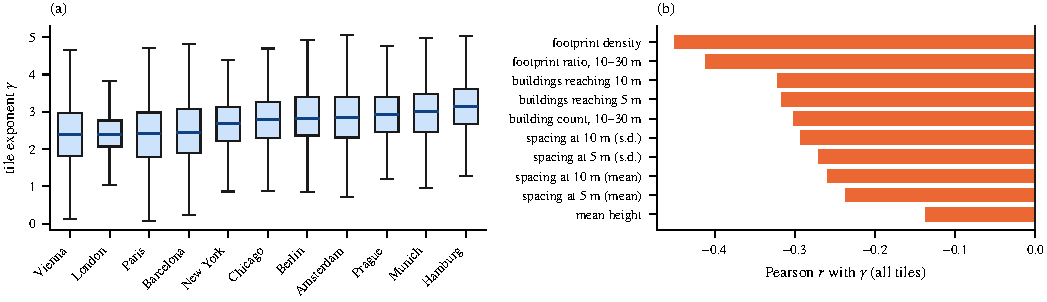
\includegraphics[width=\textwidth]{figures/fig_corpus.pdf}
\caption{(a)~Tile exponents per city (box: quartiles; whiskers: 1.5 times the
interquartile range). (b)~The ten descriptors most correlated with the tile
exponent over all \nTiles{} tiles.}
\label{fig:corpus}
\end{figure*}

The descriptors carry signal but no single one explains much of the
variation (Fig.~\ref{fig:corpus}b): the strongest correlation with the
exponent is $r=\topDescR$, for \topDesc.

\subsection{Zero-shot transfer of tile parameters}
\label{sec:res-loco}

Table~\ref{tab:loco} and Fig.~\ref{fig:loco} report the exponent error on
every held-out city under the nested protocol. The source median attains
\rmseMedian; kernel transfer \rmseKernel; the Gaussian process with learned
length scales \rmseGpArd; the learned regressors \rmseRidge{} (ridge),
\rmseMlp{} (MLP), \rmseEncoder{} (neural encoder) and \rmseGbdt{} (GBDT).
The domain-adaptation variants do not improve on their base learners (CORAL
\rmseCoral{} against ridge \rmseRidge; GBDT-IW \rmseGbdtIw{} against GBDT
\rmseGbdt), and the standard models are worse than the median (3GPP UMa
\rmseUmaLos{} for line of sight and \rmseUmaNlos{} for non-line of sight,
COST-231 Hata \rmseCost). The lowest mean error is that of the
\bestZeroShot, but the learned operators differ by less than their spread
across cities. For the intercept at \SI{\refDist}{\metre} the learned
operators reduce the error from \SI{\plRmseMedian}{\decibel} (median) to
\SI{\plRmseGbdt}{\decibel} (GBDT).

At the level of cities (Table~\ref{tab:stats-param}), GBDT changes the
error against the median by \dGbdtMedian{} (95\% CI [\loGbdtMedian,
\hiGbdtMedian], $p=\pGbdtMedian$, better in \nGbdtMedian{} of \nFolds{}
cities) and against kernel transfer by \dGbdtKernel{} ([\loGbdtKernel,
\hiGbdtKernel]); kernel transfer against the median gives \dKernelMedian{}
([\loKernelMedian, \hiKernelMedian], $p=\pKernelMedian$), whereas learning
the metric of the same kernel gives \dGpKernel{} ([\loGpKernel,
\hiGpKernel], $p=\pGpKernel$, better in \nGpKernel{} of \nFolds{} cities),
\holmGpKernel{} after Holm's correction. Over the \nZeroShotTotal{}
comparisons with the source median, \zeroShotSigBetterWord{} of the
improvements survive Holm's correction at eleven cities
(\zeroShotSigBetterList), although the learned operators are better than
the median in \learnedBetterMin{} to \learnedBetterMax{} of \nFolds{}
cities; the significant differences in the other direction are
\zeroShotSigWorseList. The hardest target is \hardCity, where the best
operator (\hardCityBestOp) reaches \hardCityBest.

\begin{table*}[!t]
\centering
\caption{Zero-shot exponent RMSE per held-out city (mean of five seeds for
stochastic operators; best per row in bold). Last row: mean $P_{L_0}$ RMSE (dB).}
\label{tab:loco}
\small
% generated by paper/scripts/make_assets.py
\begin{tabular}{lrrrrrrrrrrrrr}
\toprule
Target city & Median & UMa-L & UMa-N & COST & Kernel & GP & $k$-NN & Ridge & CORAL & MLP & Enc. & GBDT & IW \\
\midrule
Amsterdam & 0.944 & 1.146 & 1.394 & 1.042 & 0.818 & 0.784 & 0.793 & 0.780 & 0.817 & \textbf{0.776} & 0.782 & 0.786 & 0.792 \\
Barcelona & 0.999 & 0.998 & 1.730 & 1.303 & 0.811 & \textbf{0.780} & 0.800 & 0.784 & 0.823 & 0.786 & 0.786 & 0.788 & 0.787 \\
Berlin & 0.828 & 1.052 & 1.319 & 0.955 & 0.792 & \textbf{0.749} & 0.771 & 0.758 & 0.862 & 0.755 & 0.751 & 0.751 & 0.756 \\
Chicago & \textbf{0.834} & 1.006 & 1.414 & 1.030 & 0.935 & 0.893 & 0.960 & 0.879 & 0.875 & 0.892 & 0.894 & 0.885 & 0.894 \\
Hamburg & 0.844 & 1.162 & 1.078 & 0.761 & 0.645 & 0.641 & 0.627 & 0.632 & 0.637 & 0.629 & \textbf{0.620} & 0.645 & 0.651 \\
London & 0.687 & 0.639 & 1.599 & 1.110 & 0.641 & 0.642 & 0.650 & \textbf{0.635} & 0.636 & 0.650 & 0.643 & 0.661 & 0.673 \\
Munich & 0.854 & 1.120 & 1.229 & 0.881 & 0.767 & \textbf{0.756} & 0.766 & 0.765 & 0.793 & 0.764 & 0.768 & 0.758 & 0.758 \\
New York & \textbf{0.793} & 0.907 & 1.489 & 1.073 & 0.965 & 0.824 & 0.825 & 0.868 & 0.830 & 0.864 & 0.839 & 0.827 & 0.863 \\
Paris & 0.997 & 0.977 & 1.748 & 1.308 & 0.857 & \textbf{0.801} & 0.826 & 0.806 & 0.833 & 0.813 & 0.808 & 0.803 & 0.808 \\
Prague & 0.817 & 1.086 & 1.219 & 0.858 & 0.706 & 0.678 & 0.679 & 0.673 & 0.753 & \textbf{0.671} & 0.681 & 0.672 & 0.680 \\
Vienna & 0.978 & 0.938 & 1.761 & 1.311 & 0.873 & 0.836 & 0.848 & 0.836 & \textbf{0.819} & 0.843 & 0.852 & 0.829 & 0.829 \\
\midrule
Mean & 0.871 & 1.003 & 1.453 & 1.057 & 0.801 & \textbf{0.762} & 0.777 & 0.765 & 0.789 & 0.768 & 0.766 & 0.764 & 0.772 \\
S.d. & 0.098 & 0.147 & 0.234 & 0.190 & 0.107 & 0.081 & 0.096 & 0.086 & 0.082 & 0.087 & 0.087 & 0.077 & 0.079 \\
\midrule
$P_{L_0}$ (dB) & 13.8 & 21.6 & 13.8 & 17.9 & 10.2 & 9.5 & 9.7 & 9.6 & 10.3 & 9.5 & 9.6 & 9.5 & 9.5 \\
\bottomrule
\end{tabular}

\end{table*}

\begin{figure}[!t]
\centering
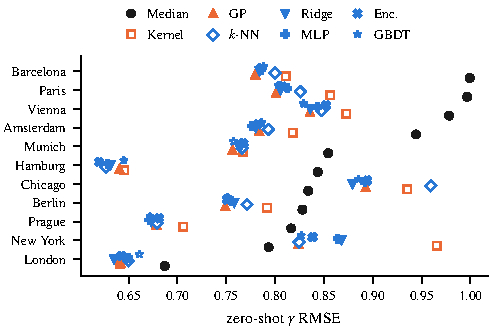
\includegraphics[width=\linewidth]{figures/fig_loco.pdf}
\caption{Zero-shot exponent RMSE per held-out city, ordered by the error of the
source median.}
\label{fig:loco}
\end{figure}

\subsection{Regime of kernel transfer}
\label{sec:res-kernel}

Table~\ref{tab:degeneracy} places the tuned kernel operator relative to
Proposition~\ref{prop:regimes}. The selected bandwidths are
$\sigma=\sigmaMin$--$\sigmaMax$ and the median $\epsilon_u$ ranges from
\epsMedianMin{} to \epsMedianMax: \fracEpsRegime\% of the target tiles
satisfy the condition of part~(a), and the largest single weight has median
\wmaxMedian, so the operator is not a nearest-neighbour copy either. Where
the largest bandwidth is selected (\nSigmaLargest{} of \nFolds{} targets),
it averages over up to \neffFracMax\% of the source tiles and its
predictions spread over as little as \spreadMin{} of the spread of the
target labels: it approaches the source mean although part~(a) does not
hold. Across the targets the prediction spread is
\spreadMin--\spreadMax{} of that of the labels. Its disadvantage is the
noise-transmission term of Eq.~\eqref{eq:decomp} combined with an isotropic
distance in which every descriptor counts equally; the Gaussian process,
which learns one length scale per descriptor, is the kernel operator that
removes most of the gap to the learned regressors
(Section~\ref{sec:res-loco}).

\begin{table}[!t]
\centering
\caption{Kernel transfer on each held-out city: selected bandwidth; median
$\epsilon_u=D_u/2\sigma^2$ and share of tiles with $\epsilon_u<1$
(Proposition~\ref{prop:regimes}a); median effective-neighbourhood fraction;
median largest weight (Proposition~\ref{prop:regimes}b); standard deviation
of the predictions over that of the labels.}
\label{tab:degeneracy}
\small\setlength{\tabcolsep}{2.5pt}
% generated by paper/scripts/make_assets.py
\begin{tabular}{lrrrrrr}
\toprule
Target & $\sigma$ & med.\ $\epsilon_u$ & $\epsilon_u{<}1$ (\%) & $n_{\mathrm{eff}}/N$ (\%) & med.\ $w_{\max}$ & spread \\
\midrule
Amsterdam & 0.2 & 78.7 & 0 & 16.42 & 0.002 & 0.41 \\
Barcelona & 0.2 & 74.8 & 0 & 19.68 & 0.001 & 0.37 \\
Berlin & 0.2 & 73.6 & 0 & 26.67 & 0.001 & 0.34 \\
Chicago & 0.1 & 306 & 0 & 0.46 & 0.061 & 0.63 \\
Hamburg & 0.2 & 75.8 & 0 & 17.04 & 0.001 & 0.45 \\
London & 0.2 & 75.5 & 0 & 24.22 & 0.001 & 0.60 \\
Munich & 0.2 & 74.9 & 0 & 29.42 & 0.001 & 0.39 \\
New York & 0.1 & 276 & 0 & 0.03 & 0.463 & 0.76 \\
Paris & 0.2 & 75.9 & 0 & 24.48 & 0.001 & 0.33 \\
Prague & 0.2 & 74.7 & 0 & 28.83 & 0.001 & 0.35 \\
Vienna & 0.2 & 73.6 & 0 & 27.56 & 0.001 & 0.32 \\
\bottomrule
\end{tabular}

\end{table}

\subsection{Few-shot correction of tile parameters}
\label{sec:res-fewshot}

Surveying target tiles helps the tile exponent little at small $k$
(Table~\ref{tab:kshot}, Fig.~\ref{fig:kshot}). The plain mean-residual
correction is worse than the zero-shot model at $k=\fsPlainWorseKs$ (GBDT at
$k=3$: \fsGbdtBiasThree{} against \fsZeroGbdt{} zero-shot): the anchors'
labels carry the site-dependent error of Section~\ref{sec:res-labels}, and
a correction fitted to a few of them adds more variance than it removes.
The empirical-Bayes correction of Eq.~\eqref{eq:fewshot}, which weights
the anchors by their precision and shrinks the correction when the inner
cities show no systematic bias, is worse than the zero-shot model
\fsEbNeverWorse{} (GBDT at $k=3$: \fsGbdtEbThree; at $k=10$: \fsTenGbdt,
\dFewEbGbdt{} against the plain correction, [\loFewEbGbdt, \hiFewEbGbdt]);
with ten random tiles it improves the GBDT error in \fsImprovedTen{} of
\nFolds{} cities, and the error falls clearly below the zero-shot value only
from $k=\fsFirstBetterK$ surveyed tiles on (GBDT \fsFirstBetterGbdt),
reaching \fsMaxGbdt{} at $k=\fsKmax$. The precision-weighted residual
model on the descriptors gives \fsGbdtResidTen{} at $k=10$. Contiguous
survey areas are worse than random tiles at every $k$ (GBDT at $k=10$:
\fsGbdtPatchTen{}), because neighbouring tiles repeat the same information.
The facility-location design, which spreads the survey over the descriptor
space without any measurement, gives \fsGbdtDesignTen{} at $k=10$
(\dFewDesignGbdt{} against random tiles, [\loFewDesignGbdt,
\hiFewDesignGbdt], better in \nFewDesignGbdt{} of \nFolds{} cities).

\begin{table}[!t]
\centering
\caption{Few-shot correction: exponent RMSE on the unsurveyed tiles, mean over
cities (and ten anchor draws for random and contiguous anchors). Left: the
empirical-Bayes correction with random anchors. Right: GBDT with the plain
bias correction, the precision-weighted residual model, contiguous anchors
and the facility-location design (all empirical Bayes unless stated).}
\label{tab:kshot}
\small\setlength{\tabcolsep}{3pt}
% generated by paper/scripts/make_assets.py
\begin{tabular}{rrrrrrrrr}
\toprule
& \multicolumn{4}{c}{EB correction, random tiles} & \multicolumn{4}{c}{GBDT} \\
\cmidrule(lr){2-5}\cmidrule(lr){6-9}
$k$ & Kernel & Ridge & MLP & GBDT & plain bias & residual & contig. & design \\
\midrule
0 & 0.801 & 0.765 & 0.768 & 0.764 & 0.764 & 0.764 & 0.764 & 0.764 \\
3 & 0.793 & 0.761 & 0.764 & 0.761 & 0.849 & 0.844 & 0.764 & 0.765 \\
5 & 0.795 & 0.763 & 0.765 & 0.763 & 0.824 & 0.818 & 0.765 & 0.762 \\
10 & 0.788 & 0.760 & 0.762 & 0.759 & 0.778 & 0.775 & 0.765 & 0.755 \\
25 & 0.781 & 0.754 & 0.756 & 0.754 & 0.758 & 0.752 & 0.771 & 0.751 \\
50 & 0.780 & 0.752 & 0.754 & 0.751 & 0.753 & 0.744 & 0.781 & 0.749 \\
100 & 0.777 & 0.751 & 0.752 & 0.750 & 0.750 & 0.739 & 0.783 & 0.753 \\
\bottomrule
\end{tabular}

\end{table}

\begin{figure*}[!t]
\centering
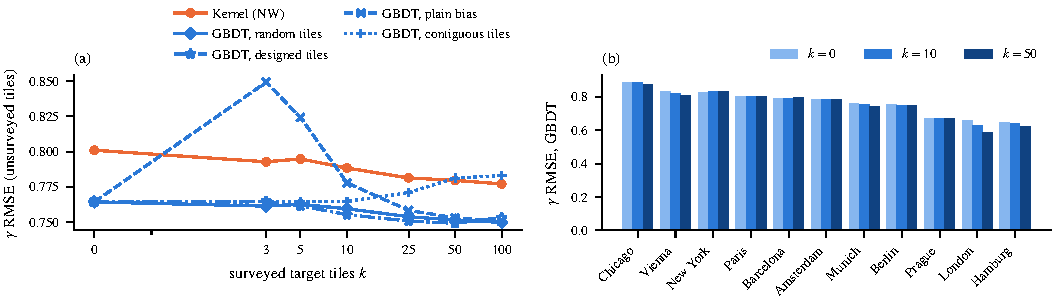
\includegraphics[width=\textwidth]{figures/fig_kshot.pdf}
\caption{(a)~Exponent RMSE against the number of surveyed target tiles.
(b)~GBDT per held-out city at $k\in\{0,10,50\}$.}
\label{fig:kshot}
\end{figure*}

\subsection{Network-level evaluation}
\label{sec:res-network}

Table~\ref{tab:network} and Fig.~\ref{fig:network} evaluate the predictors
where a planner uses them, over the complete receiver grid of the labelled
tiles. The first row is the tile model with the true labels (oracle), which
isolates the error of the tile model itself. The oracle has a path-loss error
of \SI{\netOracle}{\decibel} over the ray-traced links and
\SI{\censOracle}{\decibel} over all pairs clipped at the cut-off, selects
the correct serving site for \assocOracle\% of the pixels (the nearest-site
rule of Section~\ref{sec:netmodel}) and misjudges the SINR by
\SI{\sinrOracle}{\decibel} on average. Transferred tile parameters reduce
the path-loss error of the source median from \SI{\netMedian}{\decibel} to
\SI{\netGbdt}{\decibel} (GBDT; \dNetGbdtMedian{} dB, better in
\nNetGbdtMedian{} of \nFolds{} cities) but remain above the oracle, and a
plan of $K=5$ sites made on their map loses \regretGbdt\% of the pixels
against \regretOracle\% for the oracle.

Site-aware link transfer removes the ceiling of the tile model. Its path-loss
error is \SI{\netLink}{\decibel} (\linkMin{} to \SI{\linkMax}{\decibel}
across cities; Table~\ref{tab:link-city} lists every city),
\SI{\gainLinkGbdt}{\decibel} below tile transfer with GBDT (95\% CI
[\loNetLinkGbdt, \hiNetLinkGbdt], better in \nNetLinkGbdt{} of \nFolds{}
cities) and \SI{\gainLinkOracle}{\decibel} below the tile model with the
\emph{true} labels ([\loNetLinkOracle, \hiNetLinkOracle], \nNetLinkOracle{}
of \nFolds). It selects the correct serving site for \assocLink\% of the
pixels (\dNetLinkAssoc{} percentage points against GBDT, in
\nNetLinkAssoc{} of \nFolds{} cities), misjudges the SINR by
\SI{\sinrLink}{\decibel} on average and loses \regretLink\% of the pixels
when planning $K=5$ sites, against \regretGbdt\% for GBDT tile transfer and
\regretOracle\% for the true tile labels. Its hurdle decides the reach of
every site: it predicts the reached set of pixels correctly for
\reachLink\% of them, with a link precision of \linkPrecLink\% and a recall
of \linkRecLink\% (Table~\ref{tab:hurdle}); the regressor alone, which keeps
every link, has the same path-loss error over the ray-traced links but a
censored error of \SI{\censLinkReg}{\decibel} and a planning regret of
\regretLinkReg\%, because it lets distant, obstructed sites cover pixels
they do not reach.

\paragraph{Cell edges and dimensioning}
Table~\ref{tab:mobility} turns the maps into mobility and dimensioning
quantities. Every tile model draws the nearest-site cell pattern of
Section~\ref{sec:netmodel}: its cell edges lie \SI{\edgeGbdt}{\metre} from
the true edges on average (\SI{\edgeOracle}{\metre} with the true labels),
and their total length is in error by \edgeLenGbdt\%: the ray-traced
serving pattern is fragmented by buildings and a route crosses many more
cell edges than the nearest-site pattern suggests. Link transfer places the
edges \SI{\edgeLink}{\metre} from the truth with an edge-length error of
\edgeLenLink\%. For dimensioning, the truth needs on average
\sitesNeedTrue{} of the \nSitesPerCity{} sites to cover \covTarget\% of the
pixels at \SI{140}{\decibel}. The tile models, which cannot represent the
obstruction of distant sites, predict that \sitesNeedGbdt{} suffices
(GBDT; \sitesNeedOracle{} with the true labels, averages over the cities),
and the sites they choose cover only \sitesCovGbdt\% of the pixels in
truth. Link transfer chooses \sitesNeedLink{} on average, which cover
\sitesCovLink\%; it still under-dimensions the network, but by far less
(the regressor alone: \sitesNeedLinkReg{}, \sitesCovLinkReg\%).

The model relies on the propagation features, which account for
\linkFeatShare\% of the gain of its trees (Table~\ref{tab:importance}); the
single most important feature is the \topLinkFeat{} (\topLinkFeatShare\%),
and the three most important together account for \topThreeLinkShare\%.

\begin{table*}[!t]
\centering
\caption{Network-level evaluation on the held-out cities (mean over cities).
Oracle: tile model with the true labels. Path loss: RMSE and bias over the
ray-traced links, and RMSE over all pairs with prediction and truth clipped
at the cut-off (cens.). Serving site: share of reached pixels with the
correct serving site. Coverage: agreement of covered pixels (serving path
loss $\le\SI{130}{\decibel}$) and error of the covered share. SINR: mean
absolute error and Kolmogorov--Smirnov distance of the distributions. SE:
error of mean spectral efficiency (b/s/Hz). Regret: coverage lost by
planning $K=5$ sites on the predicted map instead of the true map. True
covered share: \covTrue\%; true mean spectral efficiency: \seTrue{}\,b/s/Hz.
Few-shot rows are scored on the unsurveyed pixels.}
\label{tab:network}
\small\setlength{\tabcolsep}{3.5pt}
% generated by paper/scripts/make_assets.py
\begin{tabular}{lrrrrrrrrrr}
\toprule
& \multicolumn{3}{c}{Path loss (dB)} & Serving & \multicolumn{2}{c}{Coverage 130\,dB (\%)} & \multicolumn{2}{c}{SINR} & SE & Regret \\
\cmidrule(lr){2-4}\cmidrule(lr){6-7}\cmidrule(lr){8-9}
Predictor & RMSE & bias & cens. & site (\%) & agree & $\Delta$ & MAE (dB) & KS & $\Delta$ & $K{=}5$ (\%) \\
\midrule
Tile labels (oracle) & 11.64 & +0.00 & 13.94 & 50.1 & 87.2 & 8.7 & 7.89 & 0.283 & \ensuremath{-}0.599 & 9.2 \\
\midrule
Source median & 14.51 & +3.72 & 15.89 & 50.1 & 83.9 & 12.9 & 7.68 & 0.269 & \ensuremath{-}0.606 & 29.8 \\
3GPP UMa NLoS & 22.75 & +17.29 & 15.35 & 50.1 & 69.2 & \ensuremath{-}14.3 & 7.56 & 0.134 & \ensuremath{-}0.164 & 9.0 \\
COST-231 Hata & 25.38 & +20.99 & 16.30 & 50.1 & 53.4 & \ensuremath{-}38.1 & 7.67 & 0.204 & \ensuremath{-}0.441 & 10.8 \\
Kernel (NW) & 12.91 & +1.16 & 14.68 & 50.1 & 84.5 & 12.4 & 7.92 & 0.275 & \ensuremath{-}0.615 & 24.3 \\
GP-ARD & 12.77 & +0.97 & 14.45 & 50.1 & 84.9 & 11.2 & 7.92 & 0.274 & \ensuremath{-}0.614 & 15.2 \\
$k$-NN & 12.80 & +1.01 & 14.53 & 50.1 & 84.9 & 12.3 & 7.97 & 0.274 & \ensuremath{-}0.611 & 32.5 \\
Ridge & 12.76 & +1.10 & 14.45 & 50.1 & 84.9 & 10.4 & 7.96 & 0.280 & \ensuremath{-}0.617 & 19.9 \\
CORAL + ridge & 13.03 & +2.18 & 14.25 & 50.1 & 84.5 & 10.2 & 7.98 & 0.292 & \ensuremath{-}0.641 & 18.4 \\
MLP & 12.75 & +0.89 & 14.50 & 50.1 & 84.8 & 11.5 & 7.95 & 0.276 & \ensuremath{-}0.613 & 24.2 \\
Neural encoder & 12.81 & +0.98 & 14.59 & 50.1 & 84.9 & 12.0 & 7.96 & 0.278 & \ensuremath{-}0.616 & 28.6 \\
GBDT & 12.75 & +0.95 & 14.52 & 50.1 & 85.0 & 11.6 & 7.93 & 0.274 & \ensuremath{-}0.614 & 18.4 \\
GBDT-IW & 12.78 & +0.94 & 14.57 & 50.1 & 85.0 & 11.5 & 7.95 & 0.275 & \ensuremath{-}0.613 & 15.5 \\
GBDT + 10 tiles & 12.73 & +0.96 & 14.48 & 50.1 & 85.1 & 11.6 & 7.93 & 0.274 & \ensuremath{-}0.612 & 19.0 \\
GBDT + 10 designed tiles & 12.74 & +1.10 & 14.40 & 50.1 & 85.0 & 11.5 & 7.92 & 0.269 & \ensuremath{-}0.600 & 16.5 \\
\midrule
Link transfer & 9.32 & +0.00 & 9.21 & 68.4 & 90.0 & 3.1 & 5.74 & 0.046 & \ensuremath{-}0.030 & 0.7 \\
Link, regressor only & 9.32 & +0.00 & 11.35 & 69.0 & 89.9 & 3.4 & 6.14 & 0.151 & \ensuremath{-}0.291 & 4.5 \\
Link + 25 tiles & 9.35 & +0.04 & 9.17 & 66.4 & 89.8 & 3.3 & 5.88 & 0.046 & \ensuremath{-}0.020 & 0.7 \\
Link + 25 tiles, stratified design & 9.41 & \ensuremath{-}0.42 & 9.23 & 65.3 & 89.5 & 4.0 & 6.04 & 0.053 & \ensuremath{-}0.019 & 0.7 \\
\bottomrule
\end{tabular}

\end{table*}

\begin{figure*}[!t]
\centering
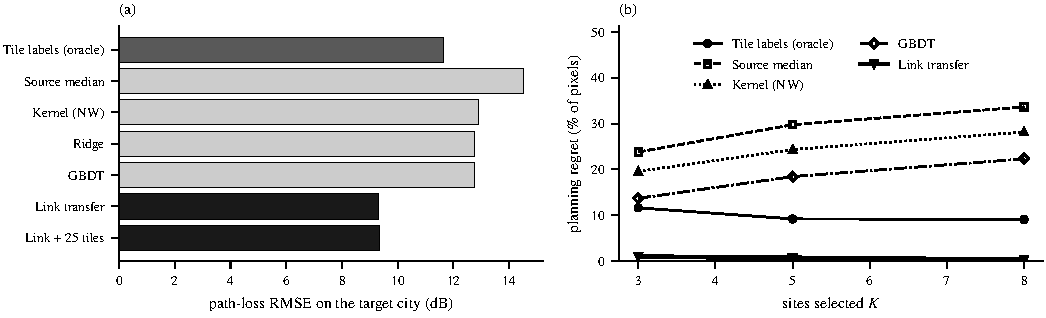
\includegraphics[width=\textwidth]{figures/fig_network.pdf}
\caption{(a)~Path-loss RMSE on the held-out cities. (b)~Planning regret against
the number of selected sites.}
\label{fig:network}
\end{figure*}

\begin{table}[!t]
\centering
\caption{Link existence. Reach: share of pixels whose reached/unreached
state is predicted correctly; precision and recall of the predicted links
below the cut-off; censored RMSE over all pairs. The tile models reach
every pixel from every site.}
\label{tab:hurdle}
\small
% generated by paper/scripts/make_assets.py
\begin{tabular}{lrrrr}
\toprule
Predictor & reach (\%) & precision (\%) & recall (\%) & cens.\ RMSE (dB) \\
\midrule
Tile labels (oracle) & 95.2 & 45.5 & 100.0 & 13.94 \\
GBDT & 95.2 & 45.5 & 100.0 & 14.52 \\
Link transfer & 95.8 & 81.7 & 79.2 & 9.21 \\
Link, regressor only & 95.2 & 45.5 & 100.0 & 11.35 \\
\bottomrule
\end{tabular}

\end{table}

\begin{table}[!t]
\centering
\caption{Per-city results of the tile model with exact labels (oracle),
GBDT tile transfer and link transfer (mean of five seeds).}
\label{tab:link-city}
\footnotesize\setlength{\tabcolsep}{2.5pt}
% generated by paper/scripts/make_assets.py
\begin{tabular}{lrrrrrrrr}
\toprule
& \multicolumn{3}{c}{Path loss (dB)} & \multicolumn{2}{c}{Serving (\%)} & \multicolumn{3}{c}{Regret $K{=}5$ (\%)} \\
\cmidrule(lr){2-4}\cmidrule(lr){5-6}\cmidrule(lr){7-9}
City & oracle & GBDT & link & oracle & link & oracle & GBDT & link \\
\midrule
Amsterdam & 11.27 & 12.12 & 9.32 & 56.3 & 69.3 & 5.4 & 20.1 & 1.1 \\
Barcelona & 11.56 & 12.57 & 9.47 & 59.4 & 68.8 & 6.5 & 5.3 & 0.7 \\
Berlin & 11.62 & 12.39 & 9.45 & 37.6 & 66.6 & 12.7 & 19.1 & 0.6 \\
Chicago & 12.73 & 14.04 & 9.28 & 40.6 & 72.9 & 8.0 & 17.8 & 1.6 \\
Hamburg & 11.44 & 12.49 & 8.97 & 57.6 & 76.9 & 1.9 & 14.6 & 0.7 \\
London & 11.22 & 13.07 & 8.83 & 52.4 & 68.9 & 10.9 & 5.6 & 1.2 \\
Munich & 11.16 & 12.14 & 9.28 & 52.3 & 68.6 & 15.8 & 14.6 & 0.4 \\
New York & 12.56 & 13.74 & 9.59 & 39.1 & 61.9 & 11.8 & 20.8 & 1.1 \\
Paris & 11.77 & 12.97 & 9.60 & 52.6 & 65.5 & 4.7 & 21.6 & 0.3 \\
Prague & 11.40 & 12.17 & 9.13 & 51.1 & 69.4 & 15.7 & 22.9 & 0.1 \\
Vienna & 11.35 & 12.60 & 9.58 & 51.6 & 64.2 & 7.8 & 40.4 & 0.0 \\
\bottomrule
\end{tabular}

\end{table}

\begin{table}[!t]
\centering
\caption{Cell edges and dimensioning (mean over held-out cities). Disp.:
mean distance between true and predicted cell edges; length: relative error
of the number of cell-edge pixels. Plan: sites chosen greedily on the
predicted map until it covers \covTarget\% of the pixels at
\SI{140}{\decibel}, and the true coverage of those sites; truth: sites the
same procedure needs on the true map.}
\label{tab:mobility}
\footnotesize\setlength{\tabcolsep}{2.5pt}
% generated by paper/scripts/make_assets.py
\begin{tabular}{lrrrr}
\toprule
& \multicolumn{2}{c}{Cell edges} & \multicolumn{2}{c}{Plan for 90\%} \\
\cmidrule(lr){2-3}\cmidrule(lr){4-5}
Predictor & disp.\ (m) & length (\%) & sites & true cov.\ (\%) \\
\midrule
Tile labels (oracle) & 76 & \ensuremath{-}92 & 1.1 & 47.8 \\
\midrule
Source median & 81 & \ensuremath{-}92 & 1.0 & 54.8 \\
3GPP UMa NLoS & 81 & \ensuremath{-}92 & 5.6 & 79.4 \\
Kernel (NW) & 81 & \ensuremath{-}92 & 1.0 & 50.8 \\
GP-ARD & 81 & \ensuremath{-}92 & 1.0 & 47.6 \\
Ridge & 81 & \ensuremath{-}92 & 1.0 & 48.6 \\
GBDT & 81 & \ensuremath{-}92 & 1.0 & 47.9 \\
GBDT + 10 tiles & 81 & \ensuremath{-}92 & 1.0 & 48.4 \\
\midrule
Link transfer & 7 & \ensuremath{-}8 & 3.6 & 80.4 \\
Link, regressor only & 7 & +5 & 1.0 & 54.9 \\
Link + 25 tiles & 8 & \ensuremath{-}8 & 3.6 & 80.4 \\
\midrule
Truth & 0 & 0 & 6.1 & 90+ \\
\bottomrule
\end{tabular}

\end{table}

\begin{table}[!t]
\centering
\caption{Link transfer: the ten features with the largest share of the total
split gain (mean over folds and seeds).}
\label{tab:importance}
\small
% generated by paper/scripts/make_assets.py
\begin{tabular}{lr}
\toprule
Feature & gain share (\%) \\
\midrule
knife-edge loss & 22.0 \\
max.\ excess height & 19.2 \\
buildings crossed & 17.5 \\
log distance & 11.9 \\
blocked fraction & 9.6 \\
length over buildings & 6.3 \\
horizontal distance & 2.4 \\
built fraction, 50\,m & 1.8 \\
receiver building height & 1.7 \\
site height & 1.5 \\
\bottomrule
\end{tabular}

\end{table}

\subsection{Where the gap comes from, and physics baselines}
\label{sec:res-decomp}

Table~\ref{tab:variants} attributes the gap between the tile model and link
transfer. Giving GBDT tile transfer the hurdle of the link model changes its
path-loss error from \SI{\varGbdtNet}{\decibel} to \SI{\varGbdtHNet}{\decibel}
over the ray-traced links, but its censored error from
\SI{\varGbdtCens}{\decibel} to \SI{\varGbdtHCens}{\decibel} and its planning
regret from \varGbdtRegret\% to \varGbdtHRegret\% (\dDecHurdleRegret{}
percentage points, [\loDecHurdleRegret, \hiDecHurdleRegret]): the cut-off,
not the path-loss accuracy, is what makes the plans of the tile models
unreliable. The dual-slope label, which gives every tile a line-of-sight and
an obstructed pair (Table~\ref{tab:los}: \losShareMin--\losShareMax\% of the
links are in line of sight; median exponents \losGammaMedian{} and
\nlosGammaMedian), lifts the nearest-site restriction and changes the
serving-site accuracy of GBDT from \varGbdtAssoc\% to \varGbdtLosAssoc\%
(\dDecLosAssoc{} points, [\loDecLosAssoc, \hiDecLosAssoc]) and the path-loss
error to \SI{\varGbdtLosNet}{\decibel}; with both, the tile model reaches
\SI{\varGbdtLosHNet}{\decibel}, \varGbdtLosHAssoc\% and a regret of
\varGbdtLosHRegret\%. With exact labels the same two additions bring the
tile model to \SI{\varOracleLosHNet}{\decibel}, \varOracleLosHAssoc\% and
\varOracleLosHRegret\%. Link transfer remains better than the best tile
variant with transferred labels (\varBestTileNet{} in path loss) in
\nLinkBetterTileNet{} of \nVarFolds{} cities in path loss, in
\nLinkBetterTileAssoc{} in serving site and in \nLinkBetterTileRegret{} in
regret (\dDecLinkBestTile{} dB, [\loDecLinkBestTile, \hiDecLinkBestTile]),
and than the dual-slope hurdle model with \emph{exact} labels by
\dDecLinkOracleLosH{} dB ([\loDecLinkOracleLosH, \hiDecLinkOracleLosH]) and
\dDecLinkOracleLosHAssoc{} points of serving site. What remains after the
cut-off and the line-of-sight state is the geometry of the individual link:
how far above the line of sight the obstruction rises, how many buildings
the path crosses and how long it runs over them, which no per-tile summary
carries.

The non-learned per-link baselines use exactly that geometry. Free space with
a single knife edge gives \SI{\varKeNet}{\decibel}, the Deygout three-edge
construction \SI{\varDeygoutNet}{\decibel} and 3GPP UMa with the geometric
line-of-sight state \SI{\varUmaGeoNet}{\decibel}; the best of them in path
loss is \varBestPhysNet{} (\varBestPhysNetVal{}\,dB), in serving site
\varBestPhysAssoc{} (\varBestPhysAssocVal\%) and in planning regret
\varBestPhysRegret{} (\varBestPhysRegretVal\%). Link transfer is better than
the best physics baseline in \nLinkBetterPhysNet{} of \nVarFolds{} cities in
path loss, in \nLinkBetterPhysAssoc{} in serving site and in
\nLinkBetterPhysRegret{} in regret; against the Deygout model the
differences are \dDecLinkDeygout{} dB ([\loDecLinkDeygout, \hiDecLinkDeygout]),
\dDecLinkDeygoutAssoc{} points of serving site and \dDecLinkDeygoutRegret{}
points of regret, and against UMa with geometric line of sight
\dDecLinkUma{} dB ([\loDecLinkUma, \hiDecLinkUma]) and \dDecLinkUmaAssoc{}
points. Of the \nDecompLinkTotal{} comparisons of link transfer with the tile
variants and the physics baselines, \nDecompLinkAllCities{} hold in every
city and \nDecompLinkHolm{} survive Holm's correction
(Table~\ref{tab:stats-net}). The learned link model thus adds to the
diffraction physics it is built on; it is not the geometry alone that
explains its advantage over the tile representation.

\begin{table}[!t]
\centering
\caption{Decomposition of the gap. Receiver-tile variants of the tile model
with exact labels, the source median and GBDT transfer, each without and with
the hurdle of the link model (+hurdle) and with a dual-slope
line-of-sight/obstructed label; non-learned per-link baselines with the
deterministic hurdle ``loss $\le$ cut-off''; and link transfer. Means over
the held-out cities; cens.: censored RMSE; reach: correctly predicted
reached/unreached pixels; cov.: coverage agreement at \SI{130}{\decibel};
regret: $K=5$.}
\label{tab:variants}
\footnotesize\setlength{\tabcolsep}{2.5pt}
% generated by paper/scripts/make_assets.py
\begin{tabular}{lrrrrrrr}
\toprule
& \multicolumn{2}{c}{Path loss (dB)} & & & & & \\
\cmidrule(lr){2-3}
Predictor & RMSE & cens. & reach (\%) & serv.\ (\%) & cov.\ (\%) & SINR (dB) & regret (\%) \\
\midrule
\multicolumn{8}{l}{\emph{Receiver tile, exact labels}} \\
Tile labels (oracle) & 11.64 & 13.94 & 95.2 & 50.1 & 87.2 & 7.89 & 9.2 \\
Tile labels + hurdle & 11.64 & 10.53 & 95.8 & 50.4 & 89.0 & 7.24 & 0.8 \\
Tile labels, dual slope & 10.02 & 12.71 & 95.2 & 61.5 & 87.2 & 7.38 & 9.5 \\
Tile labels, dual slope + hurdle & 10.02 & 9.46 & 95.8 & 61.8 & 88.9 & 6.70 & 0.7 \\
\multicolumn{8}{l}{\emph{Receiver tile, source median}} \\
Source median & 14.51 & 15.89 & 95.2 & 50.1 & 83.9 & 7.68 & 29.8 \\
Source median + hurdle & 14.51 & 11.92 & 95.8 & 50.4 & 87.1 & 7.65 & 0.7 \\
Source median, dual slope & 11.47 & 13.86 & 95.2 & 62.6 & 84.9 & 7.08 & 33.1 \\
Source median, dual slope + hurdle & 11.47 & 10.09 & 95.8 & 62.8 & 88.1 & 6.94 & 0.7 \\
\multicolumn{8}{l}{\emph{Receiver tile, GBDT transfer}} \\
GBDT & 12.75 & 14.52 & 95.2 & 50.1 & 85.0 & 7.93 & 18.4 \\
GBDT + hurdle & 12.75 & 11.19 & 95.8 & 50.4 & 87.6 & 7.48 & 0.9 \\
GBDT, dual slope & 10.97 & 13.12 & 95.2 & 62.0 & 85.3 & 7.19 & 14.9 \\
GBDT, dual slope + hurdle & 10.97 & 9.98 & 95.8 & 62.2 & 87.6 & 6.65 & 0.9 \\
\multicolumn{8}{l}{\emph{Per-link physics, no training}} \\
Free space + knife edge & 14.66 & 11.16 & 92.8 & 53.8 & 73.1 & 8.98 & 1.5 \\
Free space + Deygout & 21.66 & 11.33 & 91.3 & 55.9 & 70.3 & 9.02 & 0.1 \\
3GPP UMa, geometric LoS & 17.88 & 12.21 & 95.2 & 62.3 & 81.5 & 7.74 & 3.1 \\
\multicolumn{8}{l}{\emph{Site-aware link model}} \\
Link transfer & 9.32 & 9.21 & 95.8 & 68.4 & 90.0 & 5.74 & 0.7 \\
\bottomrule
\end{tabular}

\end{table}

\begin{table}[!t]
\centering
\caption{Dual-slope labels. Share of line-of-sight links, tiles with at
least \minLinks{} links of each kind (the others fall back to the all-link
pair), and median parameters per kind.}
\label{tab:los}
\footnotesize\setlength{\tabcolsep}{2.5pt}
% generated by paper/scripts/make_assets.py
\begin{tabular}{lrrrrrrr}
\toprule
& LoS links & \multicolumn{2}{c}{Tiles with a pair} & \multicolumn{2}{c}{med.\ $\gamma$} & \multicolumn{2}{c}{med.\ $P_{L_0}$ (dB)} \\
\cmidrule(lr){3-4}\cmidrule(lr){5-6}\cmidrule(lr){7-8}
City & (\%) & LoS & NLoS & LoS & NLoS & LoS & NLoS \\
\midrule
Amsterdam & 11.1 & 440/948 & 948/948 & 2.46 & 2.62 & 94.9 & 103.7 \\
Barcelona & 12.8 & 373/942 & 941/942 & 2.20 & 2.26 & 102.6 & 108.1 \\
Berlin & 10.9 & 672/957 & 957/957 & 2.60 & 2.61 & 82.0 & 101.8 \\
Chicago & 24.6 & 772/961 & 961/961 & 2.50 & 2.52 & 81.0 & 104.2 \\
Hamburg & 19.4 & 726/961 & 961/961 & 2.52 & 2.76 & 81.2 & 99.1 \\
London & 22.4 & 475/940 & 940/940 & 2.27 & 2.20 & 88.5 & 106.4 \\
Munich & 11.4 & 473/950 & 950/950 & 2.58 & 2.77 & 88.8 & 103.0 \\
New York & 14.2 & 581/960 & 960/960 & 2.57 & 2.41 & 83.0 & 106.6 \\
Paris & 13.2 & 326/910 & 910/910 & 2.12 & 2.26 & 104.3 & 108.5 \\
Prague & 9.8 & 575/960 & 960/960 & 2.62 & 2.76 & 82.7 & 102.3 \\
Vienna & 6.1 & 253/939 & 939/939 & 2.20 & 2.25 & 107.7 & 110.3 \\
\bottomrule
\end{tabular}

\end{table}

\subsection{Mixed-path composition}
\label{sec:res-mixed}

Composing the tile parameters along each path also lifts the nearest-site
restriction, and with exact labels it helps (Table~\ref{tab:mixed}): the
path-averaged composition, fitted to the links of each city, has a
path-loss error of \SI{\mixAvgNetOracle}{\decibel} against
\SI{\netOracle}{\decibel} for the receiver-tile labels, selects the correct
serving site for \mixAvgAssocOracle\% of the pixels against \assocOracle\%,
places the cell edges \SI{\mixAvgEdgeOracle}{\metre} from the true ones and
loses \mixAvgRegretOracle\% of the pixels when planning five sites. Most of
the gain does not survive transfer. With parameters transferred by GBDT the
path-averaged composition has a path-loss error of
\SI{\mixAvgNetGbdt}{\decibel} (receiver-tile transfer:
\SI{\netGbdt}{\decibel}; better in \mixAvgBetterRecvPl{} of \nFolds{}
cities) and a serving-site accuracy of \mixAvgAssocGbdt\%, above the
nearest-site rule in \mixAvgBetterRecvAssoc{} of \nFolds{} cities: every
link now accumulates the transfer errors of all the tiles it crosses, and
these errors decide which site appears strongest. Its planning regret is
\mixAvgRegretGbdt\% against \regretGbdt\%, still far above the
\regretLink\% of link transfer. The piecewise composition gains little over
the receiver tile even with exact labels (\SI{\mixPwNetOracle}{\decibel},
\mixPwAssocOracle\%), and with transferred exponents it is the worse of the
two (GBDT \SI{\mixPwNetGbdt}{\decibel}, \mixPwAssocGbdt\%): an error in the
exponent of one tile shifts the loss of every link that passes through it.
Larger tiles, as in~\cite{ozyurt2026}, do not change the picture
(Table~\ref{tab:mixedsize} in \ref{app:robust}): with tiles of
\SI{200}{\metre} to \SI{1000}{\metre} the path-averaged and piecewise
compositions have errors of \mixSizeAvgOracleMin{} to
\SI{\mixSizeAvgOracleMax}{\decibel} and \mixSizePwOracleMin{} to
\SI{\mixSizePwOracleMax}{\decibel} with exact labels, and
\mixSizeAvgGbdtMin{} to \SI{\mixSizeAvgGbdtMax}{\decibel} and
\mixSizePwGbdtMin{} to \SI{\mixSizePwGbdtMax}{\decibel} with GBDT. Over
all compositions and tile sizes, the best tile model with exact labels
reaches \SI{\mixSizeBestNet}{\decibel} and \mixSizeBestAssoc\% of the
serving sites, and link transfer is \mixSizeLinkBetterBest{} than it in
both; against the path-averaged composition with exact labels, link
transfer is better in \mixAvgLinkBetterPl{} of \nFolds{} cities in path
loss and in \mixAvgLinkBetterAssoc{} in serving site, and at least as good
in planning regret in \mixAvgLinkBetterRegret. The limitation lies in
describing a link by tile parameters, however they are combined and
whatever the tile size.

\begin{table}[!t]
\centering
\caption{Receiver-tile and mixed-path compositions of the tile model, and
link transfer, on the held-out cities (mean over cities). Tile labels:
fitted to the links of the held-out city itself; median, kernel and GBDT:
transferred from the training cities. PL: path-loss RMSE; serv.:
serving-site accuracy; SINR: mean absolute error; edge: cell-edge
displacement; regret: $K=5$.}
\label{tab:mixed}
\footnotesize\setlength{\tabcolsep}{3pt}
% generated by paper/scripts/make_assets.py
\begin{tabular}{lrrrrr}
\toprule
Predictor & PL (dB) & serv.\ (\%) & SINR (dB) & edge (m) & regret (\%) \\
\midrule
\multicolumn{6}{l}{\emph{Receiver tile}} \\
Tile labels (oracle) & 11.64 & 50.1 & 7.89 & 76 & 9.2 \\
GBDT & 12.75 & 50.1 & 7.93 & 81 & 18.4 \\
\multicolumn{6}{l}{\emph{Mixed path, path-averaged}} \\
Tile labels (oracle) & 11.14 & 54.1 & 7.45 & 26 & 5.1 \\
Source median & 14.25 & 50.1 & 8.15 & 81 & 29.1 \\
Kernel (NW) & 13.41 & 44.5 & 8.08 & 48 & 18.9 \\
GBDT & 13.32 & 45.1 & 8.14 & 47 & 17.3 \\
\multicolumn{6}{l}{\emph{Mixed path, piecewise (multi-slope)}} \\
Tile labels (oracle) & 11.63 & 49.1 & 7.55 & 29 & 13.8 \\
Source median & 14.12 & 50.3 & 8.01 & 80 & 29.3 \\
Kernel (NW) & 16.27 & 33.2 & 8.18 & 64 & 26.8 \\
GBDT & 16.25 & 34.3 & 8.21 & 64 & 22.3 \\
\multicolumn{6}{l}{\emph{Mixed path, summed (\ref{app:summed})}} \\
Tile labels (oracle) & 33.20 & 21.3 & 12.11 & 14 & 7.1 \\
Source median & 92.68 & 48.7 & 7.78 & 53 & 29.3 \\
Kernel (NW) & 73.20 & 48.8 & 8.76 & 45 & 29.2 \\
GBDT & 74.09 & 41.4 & 10.44 & 37 & 20.6 \\
\multicolumn{6}{l}{\emph{Site-aware link model}} \\
Link transfer & 9.32 & 68.4 & 5.74 & 7 & 0.7 \\
\bottomrule
\end{tabular}

\end{table}

\subsection{Survey design for site calibration}
\label{sec:res-survey}

Calibrating the per-site offsets of the link model from surveyed tiles
changes it little on the corpus (Table~\ref{tab:survey}, scored on the
unsurveyed pixels). With 25 random tiles and the empirical-Bayes $\kappa$
the path-loss error goes from \SI{\svPlZero}{\decibel} to
\SI{\svPlRTwentyFive}{\decibel} (\dNetLinkTwentyFive{} dB,
[\loNetLinkTwentyFive, \hiNetLinkTwentyFive], better in
\nNetLinkTwentyFive{} of \nFolds{} cities) and the serving-site accuracy
from \svAssocZero\% to \svAssocRTwentyFive\%, with the regret unchanged at
\svRegRTwentyFive\%; the estimated $\kappa$ has a median of
\kappaMedianTwentyFive{} links and reaches its ceiling, which switches the
per-site offsets off, in \kappaShareLargeTwentyFive\% of the draws. The
fixed $\kappa=\kappaLink{}$ links gives \SI{\svPlFTwentyFive}{\decibel}
(\dNetFixedKappa{} dB against the empirical-Bayes value, [\loNetFixedKappa,
\hiNetFixedKappa]). The variance design of Proposition~\ref{prop:survey}
gives \SI{\svPlDTwentyFive}{\decibel} (\dNetDesignVar{} dB against random
tiles, [\loNetDesignVar, \hiNetDesignVar]) and the stratified design
\SI{\svPlSTwentyFive}{\decibel} (\dNetDesignStrat{} dB, [\loNetDesignStrat,
\hiNetDesignStrat]); the best of the four variants at $k=25$ is
\svBestTwentyFive. The zero-shot link model has little systematic per-site
error on this corpus for a survey of this size to remove. Calibration pays
off where a systematic error exists: on the external scenes of
Section~\ref{sec:res-robust}, whose materials shift the path loss, it
removes the bias.

\begin{table*}[!t]
\centering
\caption{Per-site calibration of the link model from $k$ surveyed tiles,
scored on the unsurveyed pixels: random tiles (mean of ten draws) with the
empirical-Bayes $\kappa$ and with the fixed $\kappa=\kappaLink{}$, the
variance design of Proposition~\ref{prop:survey} and the stratified design.
PL: path-loss RMSE (dB); serv.: serving-site accuracy (\%); regret: $K=5$
(\%). Means over the held-out cities. Zero-shot link model:
\SI{\svPlZero}{\decibel}, \svAssocZero\%, \svRegZero\%.}
\label{tab:survey}
\small\setlength{\tabcolsep}{3pt}
% generated by paper/scripts/make_assets.py
\begin{tabular}{rrrrrrrrrrrrr}
\toprule
& \multicolumn{3}{c}{Random, EB $\kappa$} & \multicolumn{3}{c}{Random, fixed $\kappa$} & \multicolumn{3}{c}{Variance design} & \multicolumn{3}{c}{Stratified design} \\
\cmidrule(lr){2-4}\cmidrule(lr){5-7}\cmidrule(lr){8-10}\cmidrule(lr){11-13}
$k$ & PL & serv. & regret & PL & serv. & regret & PL & serv. & regret & PL & serv. & regret \\
\midrule
10 & 9.49 & 64.9 & 0.7 & 9.45 & 65.2 & 0.7 & 9.56 & 64.9 & 0.7 & 9.50 & 64.2 & 0.9 \\
25 & 9.35 & 66.4 & 0.7 & 9.34 & 66.4 & 0.7 & 9.56 & 64.7 & 0.8 & 9.41 & 65.3 & 0.7 \\
50 & 9.30 & 67.0 & 0.7 & 9.30 & 67.0 & 0.7 & 9.61 & 64.5 & 0.8 & 9.36 & 66.1 & 0.7 \\
\bottomrule
\end{tabular}

\end{table*}

\subsection{Certified coverage}
\label{sec:res-certified}

Table~\ref{tab:certified} applies Proposition~\ref{prop:certify}. For every
predictor the bound $\hat q_t$ holds in \certValidLink{} of \nFolds{}
cities. This count is fixed by construction (with distinct margins, the bound
of rank $j$ fails exactly in the $j$ cities with the largest $q_c$) and is a
consistency check, not evidence; the guarantee concerns a new city drawn
exchangeably with the eleven. At
$\alpha=0.1$ and \SI{140}{\decibel}, the certificate of link transfer needs a
margin of \SI{\certQLink}{\decibel} and certifies \certClaimLink\% of
the pixels, with \certFalseLink\% falsely claimed; the true covered share is
\certTrueCov\%. Tile transfer needs larger margins and certifies less: GBDT
\certClaimGbdt\% (margin \SI{\certQGbdt}{\decibel}), the source median
\certClaimMedian\% and even the true tile labels \certClaimOracle\%. The
naive claim without a margin covers almost every pixel but is wrong for
\certNaiveFalseLink\% (link) to \certNaiveFalseGbdt\% (GBDT) of them, with no
stated risk. Using the second-largest margin of the other cities ($j=2$)
lowers the confidence to \certLevelTwo{} and raises the certified share of
link transfer to \certClaimTwoLink\% (GBDT \certClaimTwoGbdt\%); the bound
then holds in \certValidTwoLink{} of \nFolds{} cities.
The falsely claimed shares stay far below $\alpha$ because the margin must
cover the worst city; the value of the certificate is the guarantee itself,
and with eleven cities its resolution is coarse: a 95\% level would need
twenty cities.

\begin{table*}[!t]
\centering
\caption{Certified coverage (Proposition~\ref{prop:certify}), mean over
held-out cities. $\hat q_t$: margin from the other cities; valid: cities in
which $q_t\le\hat q_t$ (of \nFolds); $r_p\le\hat q_t$: share of pixels within
the margin; certified claim: share claimed covered and share claimed but not
covered; naive claim: without a margin; covered: true covered share.}
\label{tab:certified}
\small\setlength{\tabcolsep}{4pt}
% generated by paper/scripts/make_assets.py
\begin{tabular}{lrrrrrrrr}
\toprule
& & & & \multicolumn{2}{c}{Certified claim} & \multicolumn{2}{c}{Naive claim} & \\
\cmidrule(lr){5-6}\cmidrule(lr){7-8}
Predictor & $\hat q_t$ (dB) & valid & $r_p\le\hat q_t$ (\%) & claimed (\%) & false (\%) & claimed (\%) & false (\%) & covered (\%) \\
\midrule
\multicolumn{9}{l}{\emph{$\alpha=0.1$, $L=\SI{140}{\decibel}$, bound holding with probability $\ge 10/11$}} \\
Tile labels (oracle) & 22.7 & 10 & 96.4 & 54.3 & 0.56 & 99.8 & 8.05 & 91.8 \\
Source median & 30.3 & 10 & 96.6 & 20.1 & 0.52 & 100.0 & 8.20 & 91.8 \\
3GPP UMa NLoS & 21.6 & 10 & 96.4 & 29.0 & 0.87 & 95.3 & 7.72 & 91.8 \\
Kernel (NW) & 25.7 & 10 & 96.4 & 42.2 & 0.45 & 100.0 & 8.20 & 91.8 \\
Ridge & 23.9 & 10 & 96.1 & 49.5 & 0.64 & 100.0 & 8.20 & 91.8 \\
GBDT & 24.1 & 10 & 95.9 & 48.4 & 0.59 & 100.0 & 8.20 & 91.8 \\
Link transfer & 13.9 & 10 & 94.9 & 80.6 & 1.31 & 95.3 & 4.89 & 91.8 \\
Link, regressor only & 16.4 & 10 & 95.4 & 75.1 & 0.74 & 100.0 & 8.20 & 91.8 \\
\multicolumn{9}{l}{\emph{$\alpha=0.1$, $L=\SI{140}{\decibel}$, bound holding with probability $\ge 9/11$}} \\
Tile labels (oracle) & 20.7 & 9 & 94.8 & 61.2 & 1.13 & 99.8 & 8.05 & 91.8 \\
Source median & 29.0 & 9 & 95.8 & 24.5 & 0.72 & 100.0 & 8.20 & 91.8 \\
3GPP UMa NLoS & 20.2 & 9 & 95.6 & 33.4 & 1.13 & 95.3 & 7.72 & 91.8 \\
Kernel (NW) & 25.2 & 9 & 95.8 & 44.1 & 0.58 & 100.0 & 8.20 & 91.8 \\
Ridge & 22.5 & 9 & 94.8 & 54.5 & 0.97 & 100.0 & 8.20 & 91.8 \\
GBDT & 23.8 & 9 & 95.3 & 49.8 & 0.74 & 100.0 & 8.20 & 91.8 \\
Link transfer & 13.0 & 9 & 94.4 & 82.6 & 1.67 & 95.3 & 4.89 & 91.8 \\
Link, regressor only & 15.9 & 9 & 94.8 & 76.2 & 0.84 & 100.0 & 8.20 & 91.8 \\
\multicolumn{9}{l}{\emph{$\alpha=0.05$, $L=\SI{140}{\decibel}$, bound holding with probability $\ge 10/11$}} \\
Tile labels (oracle) & 26.3 & 10 & 98.2 & 41.9 & 0.21 & 99.8 & 8.05 & 91.8 \\
Source median & 34.0 & 10 & 98.4 & 10.7 & 0.18 & 100.0 & 8.20 & 91.8 \\
3GPP UMa NLoS & 26.4 & 10 & 98.3 & 17.0 & 0.36 & 95.3 & 7.72 & 91.8 \\
Kernel (NW) & 29.4 & 10 & 98.4 & 28.7 & 0.14 & 100.0 & 8.20 & 91.8 \\
Ridge & 27.4 & 10 & 98.1 & 36.4 & 0.26 & 100.0 & 8.20 & 91.8 \\
GBDT & 27.6 & 10 & 98.1 & 35.9 & 0.22 & 100.0 & 8.20 & 91.8 \\
Link transfer & 18.7 & 10 & 97.5 & 69.8 & 0.40 & 95.3 & 4.89 & 91.8 \\
Link, regressor only & 19.3 & 10 & 97.6 & 68.4 & 0.34 & 100.0 & 8.20 & 91.8 \\
\bottomrule
\end{tabular}

\end{table*}

\subsection{Robustness}
\label{sec:res-robust}

\paragraph{Tile size}
Table~\ref{tab:tilesize} (\ref{app:robust}) repeats the tile pipeline for
$G_s\in\{50,100,200\}$\,m; $G_s=\SI{100}{\metre}$ reproduces the main
results exactly. Larger tiles give more precise labels (cluster-robust
standard error \tsSeFifty, \tsSeHundred{} and \tsSeTwoHundred) and a smaller
exponent error (GBDT \tsGammaFifty, \tsGammaHundred{} and \tsGammaTwoHundred),
but a coarser map: the path-loss error of the oracle goes from
\SI{\tsOracleFifty}{\decibel} to \SI{\tsOracleTwoHundred}{\decibel}, and that
of GBDT tile transfer from \SI{\tsGbdtFifty}{\decibel} to
\SI{\tsGbdtTwoHundred}{\decibel}. The serving-site accuracy of the tile model
is \tsAssocRange\% at every size, as the nearest-site rule implies. No tile
size approaches link transfer.

\paragraph{Path-loss cut-off}
Between \censMin\% and \censMax\% of the (pixel, site) pairs of the labelled
tiles lie beyond the cut-off (Table~\ref{tab:censoring}, \ref{app:robust}). The labels depend
on this dynamic range: lowering the cut-off to \SI{140}{\decibel} changes the
median tile exponent by \censDgOneForty{} and to \SI{130}{\decibel} by
\censDgOneThirty, and a Tobit fit that also uses the censored pairs gives
slopes larger than the least-squares slopes by a median of \censTobitMin{} to
\censTobitMax{} across the cities (\censTobitTiles{} tiles). The tile exponent thus
depends on the dynamic range of the measurements, not only on the
environment, which is a further reason to model links, and to model the cut-off
explicitly as the hurdle of the link model does.

\paragraph{Network size}
On the network of the first \nSitesSmall{} sites (Table~\ref{tab:density}, \ref{app:robust}),
the ranking is unchanged: the oracle has a path-loss error of
\SI{\smallNetOracle}{\decibel}, GBDT tile transfer \SI{\smallNetGbdt}{\decibel}
and link transfer \SI{\smallNetLink}{\decibel}, with serving-site accuracies
of \smallAssocOracle\%, \smallAssocGbdt\% and \smallAssocLink\%.

\paragraph{Siting and materials}
Table~\ref{tab:siting} applies the models of the main corpus, unchanged, to
the \nReplicates{} replicates (\repList) of \nRandCities{} cities
(\randCities). With sites on random rooftops (median site height
\SI{\siteHRand}{\metre} against \SI{\rsSiteHMain}{\metre} on the main
corpus) the link models reach a path-loss error of
\SI{\rsRandNetLink}{\decibel}, against \SI{\rsRandNetOracleRand}{\decibel}
for the tile model with the exact labels of the new network, with a planning
regret of \rsRandRegretLink\% against \rsRandRegretOracleRand\%. With sites
on mid-rise rooftops (median \SI{\siteHCapped}{\metre}, the 3GPP
urban-macro range) they reach \SI{\rsCappedNetLink}{\decibel} against
\SI{\rsCappedNetOracleRand}{\decibel} for the exact labels, with a regret of
\rsCappedRegretLink\% against \rsCappedRegretOracleRand\%; the link model
trained on tall sites is therefore not tied to them. With random building
materials the truth shifts by \rsMatBiasLink{}\,dB relative to the
concrete-trained link models, whose error is \SI{\rsMatNetLink}{\decibel}
against \SI{\rsMatNetOracleRand}{\decibel} for the exact labels of that
network and \SI{\rsMatNetGbdt}{\decibel} for GBDT tile transfer. The tile
labels of the same tiles fitted under the main corpus give
\SI{\rsRandNetOracleMain}{\decibel}, \SI{\rsCappedNetOracleMain}{\decibel}
and \SI{\rsMatNetOracleMain}{\decibel} on the three replicates: the labels
of a tile do not carry over to other sites or materials, as the dependence
of the exponent on the serving sites (Section~\ref{sec:res-labels})
implies.

\paragraph{Second band}
At \SI{\freqTwoGHz}{\giga\hertz} the corpus has \nSamplesTwo{} links below the
cut-off (\nTilesTwo{} labelled tiles). The tile exponents are lower than at
\SI{\freqGHz}{\giga\hertz} (median \bandGammaTwo{} against \bandGammaOne) and
the intercepts higher by a median of \SI{\bandPlShift}{\decibel}, against
\SI{\bandFsOffset}{\decibel} for free space; the per-tile exponents of the two
bands correlate with $r=\bandCorrMin$--$\bandCorrMax$ across cities. The
lower exponents agree with the stronger censoring of the higher band.
The ranking of the predictors is unchanged (Table~\ref{tab:band}): the tile
labels give \SI{\bandNetOracle}{\decibel}, GBDT tile transfer
\SI{\bandNetGbdt}{\decibel} and link transfer trained at
\SI{\freqTwoGHz}{\giga\hertz} \SI{\bandNetLink}{\decibel} (better than GBDT in
\nBandLinkGbdt{} of \nFolds{} cities). The link models trained at
\SI{\freqGHz}{\giga\hertz} transfer across bands with the free-space offset
alone: \SI{\bandNetCrossFs}{\decibel}, and \SI{\bandNetCross}{\decibel} with
the knife-edge feature evaluated at the new wavelength, both below the tile
model with the exact labels of the new band, with a serving-site accuracy of
\bandAssocCross\% and a planning regret of \bandRegretCross\%.

\paragraph{External scenes}
On the \nExtScenes{} independently modelled scenes (Table~\ref{tab:external};
\nExtLinks{} links), whose geometry and materials differ from our corpus,
zero-shot link transfer remains better than transferred tile parameters in
path loss (\SI{\extNetLink}{\decibel} against \SI{\extNetGbdt}{\decibel} for
GBDT, in \extLinkBetterGbdt{} of \nExtScenes{} scenes), serving site
(\extAssocLink\% against \extAssocGbdt\%), SINR (\SI{\extSinrLink}{\decibel}
against \SI{\extSinrGbdt}{\decibel}) and cell edges (\SI{\extEdgeLink}{\metre}
against \SI{\extEdgeGbdt}{\metre}), but its path-loss error is above that of
the tile model with the exact labels of these scenes
(\SI{\extNetOracle}{\decibel}) and it has a bias of \extLinkBiasMin{}
to \SI{\extLinkBiasMax}{\decibel} (positive in \extLinkBiasAllPositive),
consistent with the different materials of these scenes against the single
concrete model of the training corpus. This is the systematic shift that
the per-site calibration of Section~\ref{sec:link} is for: with 25 randomly
surveyed tiles the bias falls to \SI{\extBiasLinkTwentyFive}{\decibel} on
average and the path-loss error to \SI{\extNetLinkTwentyFive}{\decibel}
on the unsurveyed pixels, against \SI{\extNetOracle}{\decibel} for the exact
tile labels (lower in \extKBetterOracle{} of \nExtScenes{} scenes), while
the serving-site accuracy becomes \extAssocLinkTwentyFive\% against
\extAssocOracle\% for the tile labels. The variance design of 25 tiles
reaches \SI{\extNetLinkTwentyFiveD}{\decibel} and the stratified design
\SI{\extNetLinkTwentyFiveS}{\decibel}. With \nExtSites{} sites on these
smaller scenes, five sites cover almost every pixel, and the zero-shot
predictors have \extRegretSame{} planning regrets
(\extRegretMin--\extRegretMax\%).

\begin{table*}[!t]
\centering
\caption{Siting and materials replicates: models of the main corpus applied
to \nRandCities{} cities (\randCities) re-traced with sites on random
rooftops, with sites on mid-rise rooftops (\cappedLo--\SI{\cappedHi}{\metre})
and with random ITU materials per building. Left: the same predictors on the
main corpus of these cities. Tile labels of this network: fitted on the
replicate's links; main corpus: the labels of the same tiles in the main
corpus. PL: path-loss RMSE (dB); serv.: serving-site accuracy (\%); regret:
$K=5$ (\%). Means over cities (and seeds).}
\label{tab:siting}
\small\setlength{\tabcolsep}{3pt}
% generated by paper/scripts/make_assets.py
\begin{tabular}{lrrrrrrrrrrrr}
\toprule
& \multicolumn{3}{c}{Main corpus} & \multicolumn{3}{c}{Random rooftops} & \multicolumn{3}{c}{Mid-rise rooftops} & \multicolumn{3}{c}{Random materials} \\
\cmidrule(lr){2-4}\cmidrule(lr){5-7}\cmidrule(lr){8-10}\cmidrule(lr){11-13}
Predictor & PL & serv. & regret & PL & serv. & regret & PL & serv. & regret & PL & serv. & regret \\
\midrule
Tile labels of this network & 11.71 & 50.1 & 8.2 & 12.04 & 54.3 & 13.5 & 12.09 & 58.5 & 12.0 & 10.64 & 54.7 & 11.9 \\
Tile labels, main corpus & -- & -- & -- & 15.87 & 54.8 & 14.8 & 16.15 & 58.9 & 16.4 & 12.06 & 54.6 & 5.7 \\
Source median & 14.78 & 50.1 & 32.7 & 15.21 & 54.9 & 34.6 & 15.36 & 59.0 & 42.5 & 15.12 & 54.7 & 30.3 \\
GBDT & 12.97 & 50.1 & 17.0 & 14.81 & 54.9 & 27.4 & 14.93 & 59.0 & 25.8 & 13.60 & 54.7 & 16.4 \\
Link transfer & 9.33 & 66.4 & 0.9 & 10.82 & 64.8 & 2.0 & 11.05 & 65.6 & 0.9 & 11.07 & 66.8 & 0.3 \\
\bottomrule
\end{tabular}

\end{table*}

\begin{table}[!t]
\centering
\caption{Second band (\SI{\freqTwoGHz}{\giga\hertz}), mean over held-out cities.
Above the rule: models trained at \SI{\freqTwoGHz}{\giga\hertz}; below: the
link models trained at \SI{\freqGHz}{\giga\hertz} with the free-space offset,
with the knife-edge feature at the new wavelength or unchanged.}
\label{tab:band}
\footnotesize\setlength{\tabcolsep}{2pt}
% generated by paper/scripts/make_assets.py
\begin{tabular}{lrrrr}
\toprule
Predictor & PL (dB) & serv.\ (\%) & SINR (dB) & regret (\%) \\
\midrule
Tile labels (oracle) & 10.92 & 49.6 & 8.76 & 7.1 \\
\midrule
Source median & 13.25 & 49.8 & 8.77 & 33.0 \\
3GPP UMa NLoS & 24.88 & 49.8 & 8.93 & 7.9 \\
GBDT & 11.91 & 49.8 & 8.73 & 15.6 \\
\midrule
Link transfer & 8.51 & 65.6 & 6.45 & 0.7 \\
Link, 3.5\,GHz model & 9.07 & 68.8 & 6.73 & 1.2 \\
Link, 3.5\,GHz model, offset only & 8.98 & 68.8 & 6.70 & 1.2 \\
\bottomrule
\end{tabular}

\end{table}

\begin{table*}[!t]
\centering
\caption{External scenes of Sionna~RT (no retraining). PL: path-loss RMSE;
bias: mean path-loss error, predicted minus true (dB); serv.: serving-site
accuracy; SINR: mean absolute error; edge: cell-edge displacement; regret:
$K=5$. Tile labels: fitted on the scene itself; median, ridge and GBDT:
fitted on the eleven cities; link: mean of the eleven leave-one-city-out
link models, zero-shot and calibrated from 25 surveyed tiles (random: mean
of ten draws; the variance design; the stratified design), scored on the
unsurveyed pixels.}
\label{tab:external}
\small
% generated by paper/scripts/make_assets.py
\begin{tabular}{lrrrrrr}
\toprule
Predictor & PL (dB) & bias & serv.\ (\%) & SINR (dB) & edge (m) & regret (\%) \\
\midrule
\multicolumn{7}{l}{\emph{Munich} (104{,}696 links, 8 sites, 195 tiles)} \\
Tile labels (oracle) & 12.09 & +0.0 & 63.4 & 5.55 & 48 & 1.6 \\
Source median & 15.33 & +7.1 & 63.4 & 4.56 & 48 & 1.6 \\
Ridge & 14.64 & +3.5 & 63.4 & 4.55 & 48 & 1.6 \\
GBDT & 14.43 & +2.8 & 63.4 & 4.57 & 48 & 1.6 \\
Link transfer & 13.33 & +4.2 & 67.8 & 4.47 & 10 & 1.6 \\
Link + 25 tiles & 12.47 & +0.5 & 59.3 & 5.26 & 12 & 1.6 \\
Link + 25 tiles, variance design & 14.69 & +7.4 & 49.1 & 5.56 & 12 & 1.7 \\
Link + 25 tiles, stratified design & 12.71 & \ensuremath{-}1.9 & 62.3 & 5.00 & 11 & 1.4 \\
\multicolumn{7}{l}{\emph{\'Etoile} (42{,}235 links, 8 sites, 63 tiles)} \\
Tile labels (oracle) & 10.69 & +0.0 & 55.1 & 4.44 & 38 & 2.0 \\
Source median & 15.12 & +8.5 & 55.1 & 4.67 & 38 & 2.0 \\
Ridge & 13.87 & +2.4 & 55.1 & 4.85 & 38 & 2.0 \\
GBDT & 13.63 & +2.0 & 55.1 & 4.83 & 38 & 2.0 \\
Link transfer & 11.97 & +4.7 & 74.8 & 4.38 & 6 & 2.0 \\
Link + 25 tiles & 11.04 & \ensuremath{-}0.8 & 73.6 & 4.41 & 7 & 1.9 \\
Link + 25 tiles, variance design & 12.88 & \ensuremath{-}5.5 & 76.7 & 4.87 & 7 & 1.9 \\
Link + 25 tiles, stratified design & 12.26 & \ensuremath{-}4.4 & 74.3 & 4.68 & 7 & 2.4 \\
\multicolumn{7}{l}{\emph{Florence} (55{,}851 links, 8 sites, 127 tiles)} \\
Tile labels (oracle) & 13.93 & +0.0 & 47.6 & 7.37 & 44 & 2.2 \\
Source median & 15.51 & +1.1 & 47.6 & 6.52 & 48 & 2.2 \\
Ridge & 16.70 & +0.2 & 47.6 & 6.69 & 48 & 2.2 \\
GBDT & 16.44 & \ensuremath{-}1.0 & 47.6 & 6.61 & 48 & 2.2 \\
Link transfer & 14.14 & +2.9 & 62.3 & 6.02 & 10 & 2.2 \\
Link + 25 tiles & 13.55 & +0.0 & 57.5 & 6.89 & 14 & 2.4 \\
Link + 25 tiles, variance design & 14.49 & +6.2 & 54.6 & 7.07 & 15 & 2.5 \\
Link + 25 tiles, stratified design & 13.53 & \ensuremath{-}1.7 & 58.8 & 6.69 & 10 & 1.0 \\
\midrule
\multicolumn{7}{l}{\emph{Mean over scenes}} \\
Tile labels (oracle) & 12.24 & +0.0 & 55.4 & 5.79 & 43 & 1.9 \\
Source median & 15.32 & +5.6 & 55.4 & 5.25 & 45 & 1.9 \\
Ridge & 15.07 & +2.0 & 55.4 & 5.37 & 45 & 1.9 \\
GBDT & 14.84 & +1.2 & 55.4 & 5.34 & 45 & 1.9 \\
Link transfer & 13.14 & +3.9 & 68.3 & 4.95 & 9 & 1.9 \\
Link + 25 tiles & 12.35 & \ensuremath{-}0.1 & 63.5 & 5.52 & 11 & 2.0 \\
Link + 25 tiles, variance design & 14.02 & +2.7 & 60.1 & 5.83 & 11 & 2.0 \\
Link + 25 tiles, stratified design & 12.83 & \ensuremath{-}2.7 & 65.1 & 5.46 & 9 & 1.6 \\
\bottomrule
\end{tabular}

\end{table*}

\subsection{Statistical summary}
\label{sec:res-stats}

Tables~\ref{tab:stats-param} and~\ref{tab:stats-net} (\ref{app:stats}) list
all \nStatsRows{} city-level comparisons. Link transfer improves on GBDT
tile transfer in path loss in \nNetLinkGbdt{}, in serving site in
\nNetLinkAssoc{}, in SINR in \nNetLinkSinr{} and in planning regret in
\nNetLinkRegret{} of \nFolds{} cities, and on the tile model with the true
labels in path loss in \nNetLinkOracle{}, in serving site in
\nNetLinkOracleAssoc{} and in planning regret in \nNetLinkOracleRegret{}
of \nFolds{} cities; these comparisons are \holmNetLinkGbdt{} after Holm's
correction. At the parameter level the evidence is weaker: of the
\nZeroShotTotal{} comparisons of a transfer operator with the source
median, \nZeroShotSigBetter{} improvements survive Holm's correction at
eleven cities, whereas the gain of GP-ARD over kernel transfer is
\holmGpKernel.
%
%% ===================================================================
\section{Discussion}
\label{sec:discussion}

\paragraph{The tile exponent is not an environmental constant}
The central premise of descriptor-based tile transfer is that a tile has a
path-loss exponent determined by its environment, which can be read from
descriptors and carried to similar tiles elsewhere. On this corpus the
premise is weak, for three measured reasons. Two estimates of the same tile's
exponent from disjoint halves of the sites differ by \seSplitDiff{} in
standard deviation, so the exponent depends on which sites serve the tile;
it depends on the dynamic range of the measurements, shifting by
\censDgOneForty{} when the cut-off is lowered by \SI{10}{\decibel}; and the
cross-city spread of the city medians (\betweenSd) is small against the
spread within a city. A tile is seen by each site through a different street
canyon, and the exponent fitted over all of them mixes the geometry of the
tile with that of the paths reaching it. This explains why learned operators
improve on the source median only modestly, why few-shot correction of the
exponent needs tens of surveyed tiles before it helps, and why a planning
tool fed with even the \emph{true} receiver-tile labels assigns half of the
pixels to the wrong site and draws cell edges \SI{\edgeOracle}{\metre} away
from the true ones.

\paragraph{What the gap is made of}
Section~\ref{sec:res-decomp} separates three things that a receiver-tile
model lacks. The first is a notion of reach: without a cut-off model every
site covers every pixel, a single site appears to cover \covTarget\% of a
city, and a plan built on such a map loses \regretGbdt\% of the pixels;
the hurdle of the link model, applied to the same tile map, brings the
regret to \varGbdtHRegret\%. The second is the line-of-sight state: a
dual-slope label raises the serving-site accuracy from \varGbdtAssoc\% to
\varGbdtLosAssoc\%. The third is the geometry of the individual link, the
height of the obstruction above the line of sight, the buildings crossed
and the length over them, which the tile representation cannot carry at any
tile size and which accounts for the remaining distance to link transfer.
The per-link physics baselines, which use the same geometry without any
training, reach \SI{\varBestPhysNetVal}{\decibel} at best; the learned link
model is better than the best of them in \nLinkBetterPhysNet{} of
\nVarFolds{} cities in path loss and in \nLinkBetterPhysRegret{} in
planning regret, so the learning adds to the diffraction physics rather
than replacing it.

\paragraph{What to transfer}
The quantity that transfers is the effect of the geometry along a link,
not a per-tile summary of it. Site-aware link transfer uses the same
descriptors, the same training cities and the same protocol, but conditions
on the path between site and receiver; it improves path loss, serving site,
coverage and planning in every held-out city and outperforms the tile model
with perfect labels, however the tile parameters are composed along the
path and whatever the tile size (Section~\ref{sec:res-mixed}). It keeps its
advantage over transferred tile parameters at another frequency, with other
sites, with other building materials and on independently modelled scenes.
On the latter it is biased until a survey of 25 random tiles calibrates it,
after which its path loss is close to that of the exact tile labels and its
serving-site accuracy exceeds theirs: the material models of the training
corpus limit what transfers zero-shot, and a small unbiased survey corrects
the rest. Its most important features, the knife-edge loss and the height
of the obstruction above the line of sight, are the quantities of classical
diffraction theory~\cite{itup526}, so the model remains interpretable in
physical terms. Three design choices matter for planning. First, the model
must represent the absence of a link: the hurdle, which predicts whether a
site is received at all, reduces the planning regret from \regretLinkReg\%
to \regretLink\% at the same path-loss error over the ray-traced links.
Second, a calibration from surveyed links must be allowed to do nothing:
with the empirical-Bayes $\kappa$ the per-site offsets switch themselves
off where the survey shows no site-level bias, which a fixed prior cannot.
Third, its errors must be stated at the level of the decision: the
city-level certificate turns the leave-one-city-out residuals into a
coverage promise with a guaranteed risk, and the more accurate the model,
the more of the city it can promise (\certClaimLink\% against
\certClaimGbdt\% for tile transfer). For a 6G network digital twin this
means that the transferable representation should be attached to links (or
to site--tile pairs), which is also what a planning tool evaluates.

\paragraph{Kernel transfer}
Proposition~\ref{prop:regimes} identifies two limits of kernel transfer;
the tuned operator is in neither, but with the largest bandwidth selected
on \nSigmaLargest{} targets it approaches the source mean without reaching
the flat regime. Its disadvantage against the learned regressors is the
noise-transmission term of Eq.~\eqref{eq:decomp} combined with an
isotropic distance: learning one length scale per descriptor (GP-ARD)
removes most of the gap, which locates the weakness in the metric rather
than in kernel averaging as such.

\paragraph{Implications for planning}
Four practical conclusions follow. First, a transfer model for a
digital twin should be validated at the network level; parameter errors of
similar size lead to very different planning losses (Table~\ref{tab:network}),
and a uniformly biased model such as the 3GPP UMa NLoS constants has a
path-loss error of \SI{\netUmaNlos}{\decibel}, far above all transfer
operators, yet a planning
regret of \regretUmaNlos\%, below that of transferred tile parameters,
because a uniform bias does not change which sites cover the most pixels.
Second, models trained on links below a receiver cut-off overstate the reach
of distant sites unless the cut-off is modelled; every zero-shot tile model
with transferred parameters predicts that a single site covers \covTarget\%
of a city, and a hurdle fixes most of the planning loss even for the tile
model. Third, small surveys do not help a model without systematic error,
but correct a shifted one, and they must be unbiased: a design that
maximises the variance reduction of the offsets selects unrepresentative
tiles, and the empirical-Bayes prior should decide how much to trust them.
Fourth, coverage claims should come with a margin estimated across cities:
without it, \certNaiveFalseGbdt\% of the pixels promised by tile transfer
are not covered.

\paragraph{Limitations}
The path loss is ray traced rather than measured, so absolute values depend
on the solver, the ITU material models and the level-of-detail-1 geometry;
the results are comparisons under identical conditions, and the solver
noise floor of Section~\ref{sec:res-corpus} bounds the agreement any model
can reach near the cut-off. Ray tracing on single-material geometry makes
path loss a near-deterministic function of the obstruction geometry that
the link features encode; measured data carry variance from materials,
vegetation, vehicles and indoor clutter that a per-link geometry does not
see and that a tile statistic partly absorbs. The materials replicate and
the external scenes test the first of these and show the expected bias,
which a small survey removes; vegetation and clutter remain untested, and
none of the replicates replaces validation against measurements with known
site positions, which the public drive-test data we could obtain do not
provide. Between \impMin\% and \impMax\% of the building heights are imputed
per city. With eleven cities, city-level tests have limited power: an exact
Wilcoxon test with Holm's correction over a dozen comparisons requires
nearly every city to agree, which is why no improvement of a tile operator
over the median survives it although the learned operators improve on it in
\learnedBetterMin{} to \learnedBetterMax{} of \nFolds{} cities, and why the
certificate cannot state a 95\% level; a corpus of twenty or more cities,
which the released pipeline generates at \rtSecPerSite{}\,s per site, would
remove both limits. The corpus has flat terrain, \nSitesPerCity{} rooftop
sites per city with isotropic antennas, full load and a fixed link budget.
Tile labels come from the same ray tracer as the network truth, so the oracle
is the reference for tile models with exact labels on this corpus, not a
statement about measured data.
%
%% ===================================================================
\section{Conclusions and future work}
\label{sec:conclusion}

This article has evaluated the cross-city transfer of propagation models
for network planning in 6G digital twin networks on reproducible ray-traced
corpora of \nCities{} cities in two bands, with siting and material
replicates, and has scored every model where a planner uses it. Tile labels
of the log-distance law were shown to be ill-conditioned and, once their
correlated errors are accounted for, imprecise: the cluster-robust standard
error of the exponent is \seRatio{} times the naive one, and the exponent
depends on the serving sites, the tile size and the cut-off of the data.
Transferring tile parameters with learned regressors improves on the source
median in \nGbdtMedian{} of \nFolds{} cities, although not significantly
after correction for multiple comparisons; kernel transfer improves on it
less, and the analysis of its limiting regimes and the gain from learning
its metric locate its weakness in the isotropic distance. At the network
level, even perfect tile parameters leave a path-loss error of
\SI{\netOracle}{\decibel}, assign only \assocOracle\% of the locations to
the correct serving site and misplace the cell edges by
\SI{\edgeOracle}{\metre}. A reachability hurdle removes most of the planning
loss of the tile model and a line-of-sight dual-slope label part of the
association error; the remainder is the geometry of each link. Site-aware
hurdle link transfer, which predicts each link and whether it exists from
its obstruction geometry, reduces the path-loss error to
\SI{\netLink}{\decibel}, raises the serving-site accuracy to \assocLink\%,
lowers the planning regret in every held-out city, and outperforms the
per-link diffraction and 3GPP baselines built on the same geometry in path
loss and serving site; a city-level certificate turns its accuracy into
coverage that can be promised at a stated risk.

Future work will validate these findings on measured data with known site
positions, extend the corpora to more cities, terrain, vegetation and
antenna patterns, integrate the certified maps into the closed-loop
planning and optimisation functions of a digital twin network, and study
certificates that adapt to the target city from a small survey.
%
%% ===================================================================
\section*{CRediT authorship contribution statement}
\textbf{Abraheem Rashid:} Conceptualization, Methodology, Software, Formal
analysis, Data curation, Visualization, Writing -- original draft.
\textbf{Faisal Iradat:} Software, Validation, Investigation.
\textbf{Waseem Iqbal:} Supervision, Writing -- review \& editing.
\textbf{Yawar Abbas Bangash:} Formal analysis, Writing -- review \& editing.
\textbf{Bilgin Metin:} Supervision, Writing -- review \& editing.

\section*{Declaration of competing interest}
The authors declare that they have no known competing financial interests
or personal relationships that could have appeared to influence the work
reported in this paper.

\section*{Funding}
This research did not receive any specific grant from funding agencies in
the public, commercial, or not-for-profit sectors.

\section*{Declaration of generative AI and AI-assisted technologies in the
writing process}
During the preparation of this work the authors used Claude (Anthropic) to
assist with software development, data analysis scripting and the drafting
and editing of the manuscript text. After using this tool, the authors
reviewed and edited the content as needed and take full responsibility for
the content of the publication.

\section*{Data availability}
The code, the scene definitions, the ray-traced path-loss corpora, the tile
tables and every result file are available at
\url{https://github.com/Abraheem13/terra-net}. Running \texttt{make
reproduce} regenerates all numbers, tables and figures of this article and
the article itself (\ref{app:runtime} states the cost); \texttt{make
corpus} regenerates the ray-traced corpora. Building footprints are from
Overture Maps (release \overtureRelease{}), \copyright~OpenStreetMap
contributors, Overture Maps Foundation, under the Open Database License.
%

\bibliographystyle{elsarticle-num}
\bibliography{references}

\end{document}
